%----------------------------------------------------------------------------------------
%    Processamento de Linguagem Natural -- Dive into Deep Learning (Cap. 15)
%    Tema: DEXPI (CC BY-SA 4.0), adaptado do template da disciplina CPE727
%----------------------------------------------------------------------------------------

\documentclass[aspectratio=169,xcolor=dvipsnames]{beamer}
\usetheme{DEXPI}

\usepackage{hyperref}
\usepackage{graphicx}
\usepackage{booktabs}
\usepackage[portuguese]{babel}
\usepackage{amsmath,amssymb}

\usepackage{tikz}
\usetikzlibrary{shapes.geometric,calc,positioning,arrows.meta,matrix,fit,decorations.pathreplacing}
\usepackage{pgfplots}
\pgfplotsset{compat=1.10}
\usepackage{color}

\usepackage{listings}
\lstset{
    language=Python,
    basicstyle=\ttfamily\scriptsize,
    keywordstyle=\color{dexpiBlue}\bfseries,
    commentstyle=\color{dexpiGreenDark}\itshape,
    stringstyle=\color{dexpiRedDark},
    showstringspaces=false,
    frame=single,
    rulecolor=\color{dexpiLightBlue},
    backgroundcolor=\color{dexpiBlueLight},
    columns=fullflexible,
    keepspaces=true
}

\newcommand{\hrefcol}[2]{\textcolor{cyan}{\href{#1}{#2}}}

% Notação (segue o D2L)
\newcommand{\vv}{\mathbf{v}}
\newcommand{\uu}{\mathbf{u}}
\newcommand{\xx}{\mathbf{x}}
\newcommand{\yy}{\mathbf{y}}
\newcommand{\V}{\mathcal{V}}
\newcommand{\destaque}[1]{{\color{dexpiBlue}\textbf{#1}}}

% adicionar o numero na lista final da apresentação
\setbeamertemplate{bibliography item}{\insertbiblabel}

%----------------------------------------------------------------------------------------
%    TITLE PAGE
%----------------------------------------------------------------------------------------

\title{Processamento de Linguagem Natural}

\subtitle{Dive into Deep Learning - Capítulos 15 e 16}

\author{Pedro Ivo}
\institute{CPE727 -- Aprendizado Profundo \\ Programa de Engenharia Elétrica -- COPPE/UFRJ}
\date{\today}

%----------------------------------------------------------------------------------------
%    PRESENTATION SLIDES
%----------------------------------------------------------------------------------------

\begin{document}
\begin{frame}[plain]
    \titlepage
\end{frame}

\begin{frame}{Conteúdo da Apresentação}
    \tableofcontents
\end{frame}

%========================================================================================
%  Seção 15.1 do D2L -- Word Embedding (word2vec)
%  https://d2l.ai/chapter_natural-language-processing-pretraining/word2vec.html
%========================================================================================

%------------------------------------------------
\section{Motivação: como representar palavras?}
%------------------------------------------------

\begin{frame}{Introdução: representação de palavras por vetores}
    \begin{center}
        {\large\color{dexpiBlue}\textbf{Se um computador só entende números como ele vai entender palavras?}}
    \end{center}

    \begin{columns}[c]
        \begin{column}{0.58\textwidth}
            \begin{itemize}
                \item O PLN resolve isso mapeando cada palavra para um \destaque{vetor de números reais} (\textbf{word embedding}).
                \item Palavras com \destaque{significados parecidos} ficam \destaque{próximas} matematicamente.
                \item Esses vetores são as \textit{features} de entrada que vão alimentar os nossos modelos.
            \end{itemize}
        \end{column}
        \begin{column}{0.38\textwidth}
            \centering
            \begin{tikzpicture}[font=\scriptsize, dot/.style={circle, fill=dexpiBlue, inner sep=1.3pt}]
                \draw[-{Stealth}, gray] (0,0) -- (3.6,0);
                \draw[-{Stealth}, gray] (0,0) -- (0,2.1);
                \draw[dexpiGreenDark, dashed, rounded corners] (0.3,1.05) rectangle (1.75,1.95);
                \draw[dexpiRedDark, dashed, rounded corners] (2.0,0.15) rectangle (3.45,1.0);
                \node[dot] at (0.6,1.6) {}; \node[right] at (0.6,1.6) {man};
                \node[dot] at (0.75,1.25) {}; \node[right] at (0.75,1.25) {son};
                \node[dot] at (2.3,0.75) {}; \node[right] at (2.3,0.75) {loves};
                \node[dot] at (2.45,0.4) {}; \node[right] at (2.45,0.4) {likes};
                \node[gray, anchor=north east] at (3.6,0) {$\mathbb{R}^d$};
            \end{tikzpicture}
        \end{column}
    \end{columns}

    \vspace{0.2cm}
    \centering
    \begin{tikzpicture}[
        box/.style={draw=dexpiBlue, fill=dexpiBlueLight, rounded corners=2pt, minimum height=0.8cm, align=center, font=\small},
        arr/.style={-{Stealth}, thick, dexpiBlue}]
        \node[box] (t) {Texto\\{\scriptsize ``the man loves his son''}};
        \node[box, right=0.35cm of t] (k) {Tokens\\{\scriptsize the | man | loves | \ldots}};
        \node[box, right=0.35cm of k] (i) {Índices\\{\scriptsize 0, 1, 2, 3, 4}};
        \node[box, right=0.35cm of i, fill=dexpiLightBlue, very thick] (v) {\textbf{Vetores}\\{\scriptsize $\xx_0, \xx_1, \ldots \in \mathbb{R}^d$}};
        \node[box, right=0.35cm of v] (m) {Modelo\\{\scriptsize RNN, Transformer\ldots}};
        \draw[arr] (t) -- (k);
        \draw[arr] (k) -- (i);
        \draw[arr] (i) -- (v);
        \draw[arr] (v) -- (m);
        \node[below=0.15cm of v, font=\scriptsize, text=dexpiRedDark] {\textbf{Tema de hoje}};
    \end{tikzpicture}
\end{frame}

\begin{frame}{Primeira tentativa: vetores \textit{one-hot}}
    \begin{columns}[c]
        \begin{column}{0.5\textwidth}
            \begin{itemize}
                \item Dicionário com $N = |\V|$ palavras, indexadas de $0$ a $N-1$.
                \item A palavra de índice $i$ vira um vetor de dimensão $N$ com \textbf{1} na posição $i$ e \textbf{0} no resto.
                \item É simples de construir e não exige treinamento.
            \end{itemize}
            \begin{block}{Exemplo ($N = 5$)}
                \small
                $\V = \{\text{the}, \text{man}, \text{loves}, \text{his}, \text{son}\}$
            \end{block}
        \end{column}
        \begin{column}{0.5\textwidth}
            \centering
            \begin{tikzpicture}[font=\small]
                \matrix (M) [matrix of math nodes, nodes={minimum width=0.6cm, minimum height=0.5cm, anchor=center},
                    left delimiter={[}, right delimiter={]}, row sep=1pt, column sep=1pt, ampersand replacement=\&] {
                    1 \& 0 \& 0 \& 0 \& 0 \\
                    0 \& 1 \& 0 \& 0 \& 0 \\
                    0 \& 0 \& 1 \& 0 \& 0 \\
                    0 \& 0 \& 0 \& 1 \& 0 \\
                    0 \& 0 \& 0 \& 0 \& 1 \\
                };
                \foreach \w [count=\r] in {the, man, loves, his, son} {
                    \node[anchor=east, text=dexpiBlue] at ($(M-\r-1.west)+(-0.35,0)$) {\textbf{\w}};
                }
                \foreach \c in {1,...,5} {
                    \fill[dexpiLightBlue, opacity=0.6] ($(M-\c-\c.north west)+(0.05,-0.02)$) rectangle ($(M-\c-\c.south east)+(-0.05,0.02)$);
                }
            \end{tikzpicture}
        \end{column}
    \end{columns}
\end{frame}

\begin{frame}{Por que \textit{one-hot} é uma má escolha?}
    \begin{itemize}
        \item Uma forma natural de medir semelhança entre vetores é a \destaque{similaridade do cosseno}:
    \end{itemize}
    \begin{equation*}
        \cos(\theta) = \frac{\xx^\top \yy}{\|\xx\|\,\|\yy\|} \in [-1, 1].
    \end{equation*}
    \begin{itemize}
        \item Para dois vetores one-hot de palavras \textbf{diferentes}: $\xx^\top\yy = 0 \Rightarrow \cos(\theta) = 0$.
        \item Ou seja: \textit{``man''} é tão parecido com \textit{``son''} quanto com \textit{``the''}. \textbf{Toda palavra é ortogonal a toda outra}.
    \end{itemize}

    \begin{columns}[t]
        \begin{column}{0.48\textwidth}
            \begin{alertblock}{Problemas}
                \small
                \begin{itemize}
                    \item Não codifica \textbf{semelhança} semântica.
                    \item Dimensão $N$ enorme ($10^5$--$10^6$) e vetores esparsos.
                \end{itemize}
            \end{alertblock}
        \end{column}
        \begin{column}{0.48\textwidth}
            \begin{exampleblock}{O que queremos}
                \small
                \begin{itemize}
                    \item Vetores \textbf{densos} de dimensão $d \ll N$ (ex.: $d = 100$--$300$).
                    \item Palavras parecidas $\Rightarrow$ vetores próximos.
                \end{itemize}
            \end{exampleblock}
        \end{column}
    \end{columns}
\end{frame}


\begin{frame}{Embedding: um dicionário de números}
    \begin{columns}[T]
        \begin{column}{0.5\textwidth}
            \small
            \begin{itemize}
                \item Pense num \destaque{dicionário}: você procura a palavra e recebe uma lista de números.
                \item Esse dicionário é uma tabela $\mathbf{W}$, com \textbf{uma linha por palavra}.
            \end{itemize}

            \begin{tikzpicture}
                \node[draw=dexpiBlue, fill=dexpiBlueLight, rounded corners=3pt, thick, inner sep=4pt, align=center] {
                    $\mathbf{e}_i^\top \mathbf{W} = \mathbf{W}_{i,:}$\\[1pt]
                    {\scriptsize multiplicar pelo one-hot $=$ \destaque{selecionar a linha da palavra}}};
            \end{tikzpicture}

            \vspace{0.3cm}
            \begin{tikzpicture}[baseline=-0.6ex]
                \foreach \a in {0,45,...,315} {
                    \fill[dexpiRedDark, rotate=\a] (-0.05,0.1) rectangle (0.05,0.18);
                }
                \fill[dexpiRedDark] (0,0) circle (0.13);
                \fill[white] (0,0) circle (0.05);
            \end{tikzpicture}
            {\footnotesize Os números são \textbf{\color{dexpiRedDark}APRENDIDOS}, não escolhidos por nós.}
        \end{column}
        \begin{column}{0.48\textwidth}
            \centering
            \begin{tikzpicture}
                \node[font=\small\bfseries, text=dexpiBlue] at (3.1,5.05) {O mapa do significado};
                \matrix (W) [matrix of nodes, ampersand replacement=\&, font=\scriptsize,
                    nodes={minimum height=0.34cm, anchor=center}, column sep=2pt,
                    column 1/.style={nodes={minimum width=1.0cm}},
                    column 2/.style={nodes={minimum width=0.75cm}},
                    column 3/.style={nodes={minimum width=0.75cm}}, row 2/.style={nodes={fill=dexpiGreenLight}}] at (3.1,3.95) {
                    rei \& 1.2 \& 1.5 \\
                    gato \& $-1.0$ \& 1.5 \\
                    correr \& $-0.6$ \& $-1.2$ \\
                };
                \draw[dexpiBlue] (W.north west) rectangle (W.south east);
                \draw[dexpiBlue] (W-1-1.north east) -- (W-3-1.south east);
                \node[font=\small, text=dexpiBlue, anchor=west] at ($(W.east)+(0.05,0)$) {$\mathbf{W}$};
                \begin{axis}[
                    at={(0,0)}, anchor=south west,
                    width=6.8cm, height=3.5cm, clip=false,
                    xmin=-2.4, xmax=2.6, ymin=-2.1, ymax=2.2,
                    axis lines=middle, ticks=none,
                    xlabel={\scriptsize dim 1}, ylabel={\scriptsize dim 2}]
                    \coordinate (gatoPt) at (axis cs:-1.0,1.5);
                    \addplot[only marks, mark=*, dexpiBlue] coordinates {(1.2,1.5) (1.6,1.1) (0.9,1.0)};
                    \node[font=\scriptsize, anchor=south] at (axis cs:1.2,1.5) {rei};
                    \node[font=\scriptsize, anchor=west] at (axis cs:1.6,1.1) {rainha};
                    \node[font=\scriptsize, anchor=east] at (axis cs:0.9,1.0) {príncipe};
                    \addplot[only marks, mark=square*, dexpiGreenDark] coordinates {(-1.4,1.2) (-1.0,1.5) (-1.6,0.8)};
                    \node[font=\scriptsize, anchor=south] at (axis cs:-1.0,1.5) {gato};
                    \node[font=\scriptsize, anchor=east] at (axis cs:-1.4,1.2) {cão};
                    \node[font=\scriptsize, anchor=north] at (axis cs:-1.6,0.8) {lobo};
                    \addplot[only marks, mark=triangle*, dexpiRed] coordinates {(-0.6,-1.2) (-1.1,-1.5) (-0.4,-1.6)};
                    \node[font=\scriptsize, anchor=south] at (axis cs:-0.6,-1.2) {correr};
                    \node[font=\scriptsize, anchor=east] at (axis cs:-1.1,-1.5) {andar};
                    \node[font=\scriptsize, anchor=west] at (axis cs:-0.4,-1.6) {pular};
                \end{axis}
                \draw[-{Stealth}, thick, dexpiGreenDark] (W-2-1.west) to[out=180, in=90] ($(gatoPt)+(0,0.4)$);
            \end{tikzpicture}\par
            {\scriptsize Cada linha de $\mathbf{W}$ é um ponto ($d=2$, ilustrativo).\\
            Significados parecidos $\Rightarrow$ \destaque{pontos próximos}.}
        \end{column}
    \end{columns}
\end{frame}

%------------------------------------------------
\section{word2vec: aprendizado auto-supervisionado}
%------------------------------------------------

\begin{frame}{word2vec \cite{mikolov2013efficient, mikolov2013distributed}}
    \begin{itemize}
        \item Proposto por Mikolov et al. (Google, 2013).
        \item Mapeia cada palavra para um vetor de \destaque{tamanho fixo} que expressa melhor \textbf{similaridade} e \textbf{analogia}.
        \item Dois modelos:
        \begin{itemize}
            \item \textbf{Skip-gram}: dada a palavra central, prevê as palavras do contexto.
            \item \textbf{CBOW} (\textit{Continuous Bag of Words}): dado o contexto, prevê a palavra central.
        \end{itemize}
    \end{itemize}

    \begin{block}{Por que \textit{auto-supervisionado}?}
        Não há rótulos humanos. Os ``rótulos'' (palavras vizinhas) saem do \textbf{próprio texto}. Qualquer corpus grande (Wikipédia, notícias, livros) vira dado de treino.
    \end{block}
\end{frame}

\begin{frame}{Janela de contexto: de onde vêm os dados de treino}
    \begin{itemize}
        \item Escolhemos uma \destaque{palavra central} $w_c$ e um \destaque{tamanho de janela} $m$.
        \item As palavras a até $m$ posições de distância formam o \destaque{contexto}.
    \end{itemize}
    \vspace{0.2cm}
    \centering
    \begin{tikzpicture}[
        w/.style={draw=dexpiBlue, rounded corners=2pt, minimum width=1.6cm, minimum height=0.8cm, font=\small},
        ctx/.style={w, fill=dexpiGreenLight, draw=dexpiGreenDark},
        cen/.style={w, fill=dexpiBlue, text=white, font=\small\bfseries}]
        \node[ctx] (a) at (0,0) {the};
        \node[ctx] (b) at (2,0) {man};
        \node[cen] (c) at (4,0) {loves};
        \node[ctx] (d) at (6,0) {his};
        \node[ctx] (e) at (8,0) {son};
        \draw[decorate, decoration={brace, amplitude=5pt, mirror}, thick, dexpiGreenDark]
            ($(a.south west)+(0,-0.1)$) -- ($(b.south east)+(0,-0.1)$) node[midway, below=6pt, font=\scriptsize] {$m=2$ à esquerda};
        \draw[decorate, decoration={brace, amplitude=5pt, mirror}, thick, dexpiGreenDark]
            ($(d.south west)+(0,-0.1)$) -- ($(e.south east)+(0,-0.1)$) node[midway, below=6pt, font=\scriptsize] {$m=2$ à direita};
        \node[above=0.1cm of c, font=\scriptsize, text=dexpiBlue] {centro $w^{(t)}$};
    \end{tikzpicture}

    \vspace{0.3cm}
    \begin{columns}[t]
        \begin{column}{0.45\textwidth}
            \small
            \textbf{Pares gerados (skip-gram):}\\
            (loves $\to$ the), (loves $\to$ man),\\
            (loves $\to$ his), (loves $\to$ son)
        \end{column}
        \begin{column}{0.45\textwidth}
            \small
            \textbf{Exemplo gerado (CBOW):}\\
            (\{the, man, his, son\} $\to$ loves)
        \end{column}
    \end{columns}
    \vspace{0.2cm}
    \raggedright
    \small Deslizando o centro por $t = 1, \ldots, T$, obtemos milhões de exemplos a partir de texto bruto.
\end{frame}

%------------------------------------------------
\section{O modelo Skip-gram}
%------------------------------------------------

\begin{frame}{diferenças entre Skip-gram e CBOW}
    \centering
    \begin{tikzpicture}[
        w/.style={draw=dexpiBlue, rounded corners=2pt, minimum width=1.4cm, minimum height=0.7cm, font=\small},
        ctx/.style={w, fill=dexpiGreenLight, draw=dexpiGreenDark},
        gap/.style={w, fill=white, dashed, very thick, font=\large\bfseries, text=dexpiRed},
        cen/.style={w, fill=dexpiBlue, text=white, font=\small\bfseries},
        lbl/.style={anchor=east, font=\small\bfseries, text=dexpiBlue, align=right}]
        % Skip-gram: centro -> vizinhos
        \node[lbl] at (-1.1,0) {Skip-gram\\[-2pt]{\scriptsize\mdseries adivinhar os vizinhos}};
        \node[gap] at (0,0) {?};
        \node[gap] at (1.7,0) {?};
        \node[cen] at (3.4,0) {loves};
        \node[gap] at (5.1,0) {?};
        \node[gap] at (6.8,0) {?};
        \node[font=\scriptsize, text=dexpiGreenDark, align=left, anchor=west] at (7.8,0) {resposta:\\the, man, his, son};
        % CBOW: contexto -> centro
        \node[lbl] at (-1.1,-1.2) {CBOW\\[-2pt]{\scriptsize\mdseries completar a lacuna}};
        \node[ctx] at (0,-1.2) {the};
        \node[ctx] at (1.7,-1.2) {man};
        \node[gap] at (3.4,-1.2) {?};
        \node[ctx] at (5.1,-1.2) {his};
        \node[ctx] at (6.8,-1.2) {son};
        \node[font=\scriptsize, text=dexpiGreenDark, align=left, anchor=west] at (7.8,-1.2) {resposta:\\loves};
    \end{tikzpicture}

    \vspace{0.2cm}
    \raggedright
    \small
    \begin{itemize}
        \item \textbf{Skip-gram}: ``se eu digo \textit{futebol}, o que aparece por perto?'' (\textit{bola, gol, time}\ldots). Cada vizinho vira uma \destaque{pergunta separada}: 4 vizinhos = 4 exemplos de treino.
        \item \textbf{CBOW}: o exercício de escola ``complete a frase''. Os vizinhos entram juntos, como um \destaque{saco de palavras} (\textit{bag of words}): a ordem não importa.
    \end{itemize}

    \begin{exampleblock}{Intuição (vale para os dois)}
        \small
        Para acertar, o modelo precisa aprender quais palavras combinam com quais contextos. Palavras com os \textbf{mesmos vizinhos} acabam com \textbf{vetores parecidos}.
    \end{exampleblock}
\end{frame}

\begin{frame}{Skip-gram passo a passo}
    \centering
    \begin{tikzpicture}[
        box/.style={draw=dexpiBlue, fill=dexpiBlueLight, rounded corners=2pt, align=center, font=\scriptsize, minimum height=0.8cm},
        num/.style={circle, fill=dexpiBlue, text=white, font=\scriptsize\bfseries, inner sep=1.5pt},
        arr/.style={-{Stealth}, thick, dexpiBlue}]
        \node[draw=dexpiBlue, fill=dexpiBlue, text=white, rounded corners=2pt, font=\scriptsize\bfseries, minimum width=1.2cm, minimum height=0.6cm] (c) at (0,0) {loves};
        \node[box, minimum width=1.6cm] (v) at (2.4,0) {vetor de\\centro $\vv$};
        \node[box, minimum width=2.4cm] (s) at (5.4,0) {compara com\\\textbf{cada palavra}\\do vocabulário\\(escores)};
        \node[box, fill=dexpiGreenLight, draw=dexpiGreenDark, minimum width=2.0cm] (p) at (8.6,0) {\textbf{softmax}\\probabilidades\\dos vizinhos};
        \node[box, fill=dexpiLightBlue, minimum width=2.6cm] (r) at (11.9,0) {confere com os\\vizinhos \textbf{reais}:\\the, man, his, son};
        \draw[arr] (c) -- (v);
        \draw[arr] (v) -- (s);
        \draw[arr] (s) -- (p);
        \draw[arr] (p) -- (r);
        \node[num] at ($(v.north)+(0,0.3)$) {1};
        \node[num] at ($(s.north)+(0,0.3)$) {2};
        \node[num] at ($(p.north)+(0,0.3)$) {3};
        \node[num] at ($(r.north)+(0,0.3)$) {4};
    \end{tikzpicture}

    \vspace{0.2cm}
    \raggedright
    \small
    \begin{enumerate}
        \item \textbf{Consulta}: pega o vetor de centro da palavra do meio.
        \item \textbf{Compara}: o quanto ele combina com cada candidata (produto interno).
        \item \textbf{Normaliza}: a softmax transforma os escores em probabilidades.
        \item \textbf{Confere}: quanto de probabilidade o modelo deu a cada vizinho verdadeiro?
    \end{enumerate}

    \begin{block}{Guarde para depois: o CBOW}
        \small
        Mesmo processo, mas \textbf{sem a média}: entra um vetor só e o palpite é conferido contra \textbf{vários} vizinhos.
    \end{block}
\end{frame}


\begin{frame}{A fórmula do skip-gram}
    \begin{equation*}
        P(\text{vizinho} \mid \text{centro}) =
        \frac{\exp\left({\color{dexpiBlue}\uu_o}^\top {\color{dexpiGreenDark}\vv_c}\right)}
             {{\color{dexpiRedDark}\sum_{i \in \V}} \exp\left(\uu_i^\top {\color{dexpiGreenDark}\vv_c}\right)}
    \end{equation*}

    \begin{columns}[t]
        \begin{column}{0.48\textwidth}
            \begin{block}{Lendo a fórmula}
                \small
                \begin{itemize}
                    \item {\color{dexpiGreenDark}$\vv_c$}: vetor de centro (passo 1).
                    \item {\color{dexpiBlue}$\uu_o$}: vetor da candidata a vizinha; o produto dá o escore (passo 2).
                    \item {\color{dexpiRedDark}$\sum$}: soma sobre todas as palavras = softmax (passo 3).
                \end{itemize}
            \end{block}
        \end{column}
        \begin{column}{0.48\textwidth}
            \begin{block}{Prévia do CBOW}
                \small
                O CBOW usará \textbf{esta mesma fórmula}, só trocando $\vv_c$ pela \textbf{média} dos vetores do contexto.
            \end{block}
        \end{column}
    \end{columns}

    \vspace{0.2cm}
    \small
    É uma classificação com $N$ classes: ``qual das $N$ palavras do vocabulário é a vizinha?''
\end{frame}

\begin{frame}{Como o modelo aprende: da probabilidade à perda}
    \small
    \begin{itemize}\setlength{\itemsep}{0pt}
        \item O modelo ajusta os vetores $\vv_i$ e $\uu_i$ de \textbf{todas} as palavras do vocabulário.
        \item A meta: dar \textbf{alta probabilidade} aos vizinhos que de fato aparecem no texto (\destaque{máxima verossimilhança}).
    \end{itemize}

    \vspace{0.1cm}
    {\centering
    \begin{tikzpicture}[
        passo/.style={draw=#1, fill=#1!10, line width=0.8pt, rounded corners=4pt,
                      text width=0.28\textwidth, minimum height=2.3cm, align=center, inner sep=3pt},
        seta/.style={-{Stealth[length=2.5mm]}, line width=1pt, dexpiBlueDark}]
        \node[passo=dexpiBlue] (p1) {%
            {\color{dexpiBlue}\large$\prod$\; \small\textbf{Passo 1: o produto}}\\[1pt]
            \footnotesize$\prod_{t}\prod_{j} P\big(w^{(t+j)} \mid w^{(t)}\big)$\\[1pt]
            \scriptsize Multiplica as probabilidades de \textbf{todos} os pares (centro $t$, vizinho $j$).\\[1pt]
            {\color{dexpiBlue}\scriptsize\textbf{maximizar}}};
        \node[passo=dexpiGreenDark, right=0.45cm of p1] (p2) {%
            {\color{dexpiGreenDark}\large$\log$\; \small\textbf{Passo 2: o log}}\\[1pt]
            \footnotesize$\sum_{t}\sum_{j} \log P\big(w^{(t+j)} \mid w^{(t)}\big)$\\[1pt]
            \scriptsize Transforma multiplicação em \textbf{soma} e evita números minúsculos.\\[1pt]
            {\color{dexpiGreenDark}\scriptsize\textbf{maximizar} (mesmo ótimo)}};
        \node[passo=dexpiRedDark, right=0.45cm of p2] (p3) {%
            {\color{dexpiRedDark}\large$-$\; \small\textbf{Passo 3: o negativo}}\\[1pt]
            \footnotesize$\mathcal{L} = -\sum_{t}\sum_{j} \log P\big(w^{(t+j)} \mid w^{(t)}\big)$\\[1pt]
            \scriptsize ``Maximizar o acerto'' vira ``\textbf{minimizar o erro}'' (= entropia cruzada).\\[1pt]
            {\color{dexpiRedDark}\scriptsize\textbf{minimizar}}};
        \draw[seta] (p1) -- (p2);
        \draw[seta] (p2) -- (p3);
    \end{tikzpicture}\par}

    \vspace{0.1cm}
    \begin{exampleblock}{O que é $P\big(w^{(t+j)} \mid w^{(t)}\big)$?}
        \footnotesize
        É a \textbf{similaridade} entre os vetores ($\uu_o^\top \vv_c$) passada pelo \destaque{softmax}: a fórmula do slide anterior.
    \end{exampleblock}
\end{frame}

\begin{frame}{Otimizando com SGD: um par de palavras por vez}
    \small
    A perda mede o erro; falta saber \destaque{para que lado} empurrar cada vetor (o \textbf{gradiente}). Com bilhões de palavras, cada passo usa um \textbf{trecho curto}: \destaque{SGD}.

    \vspace{0.15cm}
    {\centering
    \begin{tikzpicture}[
        carta/.style={draw=#1, fill=#1!8, line width=0.8pt, rounded corners=4pt,
                      text width=0.27\textwidth, minimum height=1.55cm, align=center, inner sep=3pt},
        seta/.style={-{Stealth[length=2.5mm]}, line width=1pt, dexpiBlueDark}]
        \node[carta=dexpiBlue] (c1) {%
            {\color{dexpiBlue}\large\textbf{1}}\;\; \small\textbf{um trecho}\\[1pt]
            {\footnotesize cada passo olha}\\[0pt]
            {\footnotesize um \textbf{lote} pequeno}\\[1pt]
            {\color{dexpiBlue}\scriptsize estocástico $=$ sorteado}};
        \node[carta=dexpiGreenDark, right=0.45cm of c1] (c2) {%
            {\color{dexpiGreenDark}\large\textbf{2}}\;\; \small\textbf{um par}\\[1pt]
            {\footnotesize bastam \textbf{dois} vetores:}\\[0pt]
            {\footnotesize centro e vizinho}\\[1pt]
            {\color{dexpiGreenDark}\scriptsize $\log P(w_o \mid w_c)$}};
        \node[carta=dexpiRedDark, right=0.45cm of c2] (c3) {%
            {\color{dexpiRedDark}\large\textbf{3}}\;\; \small\textbf{um passo}\\[1pt]
            {\footnotesize anda no sentido}\\[0pt]
            {\footnotesize que \textbf{diminui} a perda}\\[1pt]
            {\color{dexpiRedDark}\scriptsize $\vv \leftarrow \vv - \eta\,\nabla$}};
        \draw[seta] (c1) -- (c2);
        \draw[seta] (c2) -- (c3);
    \end{tikzpicture}\par}

    \vspace{0.2cm}
    {\centering
    $\log P(w_o \mid w_c) =
     \underbrace{{\color{dexpiBlue}\uu_o^\top \vv_c}}_{\text{nota do vizinho real}}
     \;-\;
     \underbrace{{\color{dexpiRedDark}\log\Big(\sum_{i \in \V} \exp(\uu_i^\top \vv_c)\Big)}}_{\text{soma sobre o vocabulário}}$
    \par}

    \vspace{0.15cm}
    \begin{exampleblock}{Uma metade premia, a outra pune}
        \footnotesize
        A {\color{dexpiBlue}nota do vizinho real} quer subir; a {\color{dexpiRedDark}soma} pune qualquer nota alta, inclusive a das palavras erradas.
    \end{exampleblock}
\end{frame}

\begin{frame}{O gradiente: observado menos esperado}
    \footnotesize
    Derivar o termo do slide anterior usa só duas regras que já conhecemos:
    \quad
    $\dfrac{\partial}{\partial \vv_c}\big(\uu_o^\top \vv_c\big) = \uu_o$
    \quad e \quad
    $\dfrac{\partial}{\partial \vv_c}\log\sum_{i \in \V}\exp(\uu_i^\top \vv_c) = \sum_{j \in \V} P(w_j \mid w_c)\,\uu_j$.

    \vspace{0.15cm}
    {\centering
    $\nabla_{\vv_c}\log P(w_o \mid w_c) =
     \underbrace{{\color{dexpiBlue}\uu_o}}_{\text{observado}}
     \;-\;
     \underbrace{{\color{dexpiRedDark}\sum_{j \in \V} P(w_j \mid w_c)\,\uu_j}}_{\text{esperado pelo modelo}}$
    \par}

    \vspace{0.1cm}
    \begin{columns}[T]
        \begin{column}{0.53\textwidth}
            \begin{block}{Lendo o resultado}
                \footnotesize
                \begin{itemize}\setlength{\itemsep}{1pt}
                    \item Se o modelo já acerta, esperado $\approx$ observado e $\nabla \approx 0$: não há o que corrigir.
                    \item A soma percorre as $N$ palavras do vocabulário, a cada par: é o custo que a Seção 15.2 resolve.
                \end{itemize}
            \end{block}
        \end{column}
        \begin{column}{0.43\textwidth}
            \centering
            \begin{tikzpicture}[scale=1.75, font=\scriptsize]
                \draw[gray!55, -{Stealth}] (-1.2,0) -- (1.3,0);
                \draw[gray!55, -{Stealth}] (0,-0.45) -- (0,1.2);
                \node[circle, fill=gray!55, inner sep=1.6pt] (man) at (0,1) {};
                \node[left=3pt of man] {man};
                \node[circle, fill=gray!55, inner sep=1.6pt] (the) at (-1,0) {};
                \node[above=2pt of the] {the};
                \node[circle, fill=dexpiBlue, inner sep=1.7pt] (son) at (1,0) {};
                \node[below right=1pt and 1pt of son, text=dexpiBlue] {son};
                \node[circle, draw=dexpiBlue, fill=white, inner sep=1.4pt] (esp) at (0.56,0.26) {};
                \node[above left=2pt and 0pt of esp, text=dexpiBlue] {esperado};
                \draw[-{Stealth}, very thick, dexpiBlue] (esp) -- (son);
                \node[above right=0pt and 3pt of son, text=dexpiBlue] {$\nabla$};
            \end{tikzpicture}\par
            \vspace{0.05cm}
            {\scriptsize A seta vai do que o modelo \textbf{esperava} até o vizinho que \textbf{apareceu}.}
        \end{column}
    \end{columns}
\end{frame}

%------------------------------------------------
\section{O modelo CBOW}
%------------------------------------------------

\begin{frame}{CBOW passo a passo}
    \centering
    \begin{tikzpicture}[
        ctx/.style={draw=dexpiGreenDark, fill=dexpiGreenLight, rounded corners=2pt, minimum width=1.2cm, minimum height=0.5cm, font=\scriptsize},
        box/.style={draw=dexpiBlue, fill=dexpiBlueLight, rounded corners=2pt, align=center, font=\scriptsize, minimum height=0.8cm},
        num/.style={circle, fill=dexpiBlue, text=white, font=\scriptsize\bfseries, inner sep=1.5pt},
        arr/.style={-{Stealth}, thick, dexpiBlue}]
        % passo 1
        \foreach \t [count=\i from 0] in {the, man, his, son} {
            \node[ctx] (c\i) at (0, 0.9-\i*0.6) {\t};
            \node[box, minimum height=0.5cm, right=0.4cm of c\i] (v\i) {vetor};
            \draw[arr] (c\i) -- (v\i);
        }
        % passo 2
        \node[box, fill=dexpiLightBlue, minimum width=2.0cm] (m) at (5.2,0) {\textbf{média}\\``resumo do\\contexto''};
        \foreach \i in {0,...,3} { \draw[arr] (v\i.east) -- (m.west); }
        % passo 3
        \node[box, minimum width=2.4cm] (s) at (8.6,0) {compara com\\\textbf{cada palavra}\\do vocabulário\\(escores)};
        \draw[arr] (m) -- (s);
        % passo 4
        \node[box, fill=dexpiGreenLight, draw=dexpiGreenDark, minimum width=2.2cm] (p) at (12.0,0) {\textbf{softmax}\\probabilidades\\$\Rightarrow$ ``loves''};
        \draw[arr] (s) -- (p);
        % números
        \node[num] at (1.4,1.45) {1};
        \node[num] at ($(m.north)+(0,0.3)$) {2};
        \node[num] at ($(s.north)+(0,0.3)$) {3};
        \node[num] at ($(p.north)+(0,0.3)$) {4};
    \end{tikzpicture}

    \vspace{0.2cm}
    \raggedright
    \small
    \begin{enumerate}
        \item \textbf{Consulta}: pega o vetor de cada palavra do contexto na tabela de embeddings.
        \item \textbf{Resume}: tira a média, um único vetor que ``representa o contexto''.
        \item \textbf{Compara}: o quanto o resumo combina com cada candidata (produto interno).
        \item \textbf{Normaliza}: a softmax transforma os escores em probabilidades.
    \end{enumerate}
\end{frame}


\begin{frame}{A fórmula do CBOW}
    \begin{equation*}
        P(\text{centro} \mid \text{contexto}) =
        \frac{\exp\left({\color{dexpiBlue}\uu_c}^\top {\color{dexpiGreenDark}\bar{\vv}_o}\right)}
             {{\color{dexpiRedDark}\sum_{i \in \V}} \exp\left(\uu_i^\top {\color{dexpiGreenDark}\bar{\vv}_o}\right)}
        \qquad \text{com} \quad {\color{dexpiGreenDark}\bar{\vv}_o} = \frac{\vv_{o_1} + \cdots + \vv_{o_{2m}}}{2m}
    \end{equation*}

    \begin{columns}[t]
        \begin{column}{0.48\textwidth}
            \begin{block}{Lendo a fórmula}
                \small
                \begin{itemize}
                    \item {\color{dexpiGreenDark}$\bar{\vv}_o$}: o resumo do contexto (passo 2).
                    \item {\color{dexpiBlue}$\uu_c$}: o vetor da candidata; o produto dá o escore (passo 3).
                    \item {\color{dexpiRedDark}$\sum$}: soma sobre todas as palavras = softmax (passo 4).
                \end{itemize}
            \end{block}
        \end{column}
        \begin{column}{0.48\textwidth}
            \begin{block}{Relação com o skip-gram}
                \small
                \textbf{É a mesma fórmula!} Só troca o vetor do centro pela \textbf{média} dos vetores do contexto.
            \end{block}
        \end{column}
    \end{columns}

    \vspace{0.1cm}
    \begin{exampleblock}{Cuidado com a notação do D2L}
        \footnotesize
        No CBOW o livro inverte as letras: $\vv$ são os vetores das palavras de \textbf{contexto} (a entrada) e $\uu_c$ é o vetor do \textbf{centro} previsto. Regra para não se perder: $\vv$ é sempre o vetor de quem \textbf{entra} no modelo.
    \end{exampleblock}
\end{frame}

\begin{frame}{Treinando o CBOW: a mesma perda, um termo por posição}
    \small
    \begin{itemize}\setlength{\itemsep}{1pt}
        \item A mesma receita de antes: \destaque{máxima verossimilhança}, $\log$ e sinal de menos.
        \item O que muda é \textbf{quantos termos} cada posição do texto gera.
    \end{itemize}

    \vspace{0.1cm}
    \begin{columns}[c]
        \begin{column}{0.48\textwidth}
            \begin{block}{Skip-gram: $2m$ termos}
                \footnotesize
                $\mathcal{L} = -\sum_{t}\sum_{j \neq 0} \log P(w^{(t+j)}\mid w^{(t)})$
                \\[2pt]
                Um termo para \textbf{cada vizinho} da janela ($-m \le j \le m$, $j \neq 0$): com $m = 2$, são \destaque{4} termos.
            \end{block}
        \end{column}
        \begin{column}{0.48\textwidth}
            \begin{block}{CBOW: \textbf{1} termo}
                \footnotesize
                $\mathcal{L} = -\sum_{t} \log P(w^{(t)}\mid C^{(t)})$
                \\[2pt]
                O contexto $C^{(t)}$ entra todo \textbf{junto}, como um saco de palavras: com $m = 2$, é \destaque{1} termo.
            \end{block}
        \end{column}
    \end{columns}

    \vspace{0.15cm}
    \begin{exampleblock}{O que se ganha e o que se perde}
        \footnotesize
        \textbf{Ganha}: menos termos por posição $\Rightarrow$ treino mais rápido. \quad
        \textbf{Perde}: a média ignora a ordem das palavras --- é o preço do ``saco de palavras''.
    \end{exampleblock}
\end{frame}

\begin{frame}{O gradiente do CBOW: o mesmo, dividido por $2m$}
    \small
    \begin{itemize}\setlength{\itemsep}{1pt}
        \item O log do CBOW é o do skip-gram trocando $\vv_c$ por $\bar{\vv}_o$; então a derivada também é a mesma. A novidade é derivar a \textbf{média} (aqui $C$ é o contexto da posição).
    \end{itemize}
    \vspace{0.05cm}
    {\centering
    $\frac{\partial \log P(w_c \mid C)}{\partial \vv_{o_i}} =
     \frac{1}{2m}\Big(
     \underbrace{{\color{dexpiBlue}\uu_c}}_{\text{observado}} -
     \underbrace{{\color{dexpiRedDark}\sum_{j \in \V} P(w_j \mid C)\,\uu_j}}_{\text{esperado pelo modelo}}\Big)$
    \par}

    \vspace{0.2cm}
    {\centering
    \begin{tikzpicture}[
        caixa/.style={draw=#1, fill=#1!8, rounded corners=3pt, line width=0.8pt,
                      text width=0.26\textwidth, minimum height=1.45cm, align=center, inner sep=3pt},
        seta/.style={-{Stealth[length=2.5mm]}, line width=1pt, dexpiBlueDark}]
        \node[caixa=dexpiBlue] (b1) {%
            \footnotesize$\bar{\vv}_o = \frac{1}{2m}\sum_{i=1}^{2m}\vv_{o_i}$\\[2pt]
            {\scriptsize resumo do contexto}};
        \node[caixa=dexpiGreenDark, right=0.45cm of b1] (b2) {%
            \footnotesize$\frac{\partial \bar{\vv}_o}{\partial \vv_{o_i}} = \frac{1}{2m}$\\[2pt]
            {\scriptsize cada palavra pesa $1/2m$}};
        \node[caixa=dexpiRedDark, right=0.45cm of b2] (b3) {%
            \footnotesize o ajuste chega \textbf{repartido}\\[2pt]
            {\scriptsize entre as $2m$ palavras do contexto}};
        \draw[seta] (b1) -- (b2);
        \draw[seta] (b2) -- (b3);
    \end{tikzpicture}\par}

    \vspace{0.15cm}
    \begin{exampleblock}{O que isso muda na prática}
        \footnotesize
        Todas as palavras do contexto são puxadas \textbf{na mesma direção}, com um passo menor. É por isso que o CBOW dilui palavras raras: elas aparecem poucas vezes e sempre dentro de uma média.
    \end{exampleblock}
\end{frame}

%------------------------------------------------
\section{Implementação e resumo}
%------------------------------------------------

\begin{frame}[fragile]{Implementação mínima em PyTorch (softmax completa)}
\begin{columns}[T]
    \begin{column}{0.62\textwidth}
\begin{lstlisting}[basicstyle=\ttfamily\fontsize{7}{8}\selectfont,aboveskip=0pt,belowskip=0pt]
class SkipGram(nn.Module):
    def __init__(self, vocab, dim):
        super().__init__()
        self.V = nn.Embedding(vocab, dim)  # centro
        self.U = nn.Embedding(vocab, dim)  # contexto

    def forward(self, center):
        v = self.V(center)          # (B, d)
        return v @ self.U.weight.T  # (B, N)

model = SkipGram(10_000, 100)
opt = torch.optim.SGD(model.parameters(), 0.01)

logits = model(center)
loss = F.cross_entropy(logits, context)
loss.backward(); opt.step()
emb = model.V.weight            # vetor final
\end{lstlisting}
    \end{column}
    \begin{column}{0.34\textwidth}
        \footnotesize
        \textbf{Onde está cada passo}\\[2pt]
        \begin{enumerate}\setlength{\itemsep}{2pt}
            \item \textbf{Consulta}: \texttt{self.V(center)}.
            \item \textbf{Compara}: \texttt{v @ U.weight.T} mede a afinidade com as $N$ palavras.
            \item \textbf{Normaliza}: a \texttt{cross\_entropy} já aplica a softmax e o $-\log$.
            \item \textbf{Confere}: o alvo \texttt{context} é o vizinho real.
        \end{enumerate}
        \vspace{0.1cm}
        {\scriptsize\color{dexpiRedDark} \textbf{O gargalo:} $N = 10^4$ já são $10^4$ contas por par. É o que a próxima seção resolve.}
    \end{column}
\end{columns}
\end{frame}

%========================================================================================
%  Seção 15.2 do D2L -- Approximate Training
%  https://d2l.ai/chapter_natural-language-processing-pretraining/approx-training.html
%========================================================================================

%------------------------------------------------
\section{Treinamento aproximado}
%------------------------------------------------

\begin{frame}{Negative Sampling e Hierarchical Softmax}
    \small
    \begin{itemize}
        \item São estratégias  para resolver problemas de lentidão no treinamento de word embeddings:
    \end{itemize}
    \vspace{-0.1cm}


    \begin{columns}[t]
        \begin{column}{0.48\textwidth}
            \begin{block}{Amostragem negativa}
                \footnotesize
                Compara a palavra certa (exemplo positivo) com apenas um pequeno grupo de palavras erradas sorteadas ao acaso (exemplos negativos), em vez de olhar o dicionário inteiro.
            \end{block}
        \end{column}
        \begin{column}{0.48\textwidth}
            \begin{block}{Softmax hierárquica}
                \footnotesize
                Organiza todo o dicionário dentro de uma árvore binária, transformando o problema em uma sequência de escolhas de "sim ou não".
            \end{block}
        \end{column}
    \end{columns}

    \note{
        Até aqui, o skip-gram e o CBOW usaram a softmax completa. Vamos olhar o custo dela com um exemplo: na janela ``o gato miou'', a palavra central é ``gato'' e as vizinhas são ``o'' e ``miou''.
        Para calcular a probabilidade de ``miou'' dado ``gato'', o numerador é barato: um único produto escalar. O problema é o denominador, que soma a exponencial do escore de \textit{todas} as palavras do dicionário. Com um vocabulário de 100 mil a 1 milhão de palavras, isso significa 100 mil a 1 milhão de produtos escalares para um único par.
        E isso se repete para cada vizinho de cada posição do corpus, que tem bilhões de palavras. É inviável.
        A Seção 15.2 do livro apresenta duas formas de aproximar esse cálculo: a amostragem negativa, que compara a palavra certa só com algumas palavras sorteadas, e a softmax hierárquica, que organiza o dicionário numa árvore. Vamos ver as duas.
    }
\end{frame}

\begin{frame}{Amostragem negativa}
    \small
    \begin{itemize}
        \item O modelo aprende a distinguir a palavra correta de $K$ \textbf{palavras de ruído} sorteadas ao acaso.
    \end{itemize}
    \centering
    \begin{tikzpicture}[
        w/.style={draw=dexpiBlue, rounded corners=2pt, minimum width=1.6cm, minimum height=0.6cm, font=\small},
        real/.style={w, fill=dexpiGreenLight, draw=dexpiGreenDark},
        neg/.style={w, fill=dexpiRedLight, draw=dexpiRedDark},
        cen/.style={w, fill=dexpiBlue, text=white, font=\small\bfseries}]
        \node[real] (p) at (0,0) {miou};
        \node[cen] (c) at (3.2,0) {gato};
        \node[neg] (n1) at (6.4,0) {avião};
        \node[neg] (n2) at (8.6,0) {cloreto};
        \draw[-{Stealth}, thick, dexpiGreenDark] (c) -- node[above, font=\scriptsize] {$D = 1$} (p);
        \draw[-{Stealth}, thick, dexpiRedDark, dashed] (c) -- node[above, font=\scriptsize] {$D = 0$} (n1);
        \draw[-{Stealth}, thick, dexpiRedDark, dashed] (c.south) to[bend right=18] node[below, font=\scriptsize] {$D = 0$} (n2.south);
    \end{tikzpicture}

    \vspace{0.1cm}
    \raggedright
    \begin{columns}[t]
        \begin{column}{0.48\textwidth}
            \begin{exampleblock}{1 exemplo positivo ($D = 1$)}
                \footnotesize
                A palavra \textbf{real} do contexto. Ex.: (gato, miou).
            \end{exampleblock}
        \end{column}
        \begin{column}{0.48\textwidth}
            \begin{alertblock}{$K$ exemplos negativos ($D = 0$)}
                \footnotesize
                Ruído que \textbf{não} está no contexto. Ex.: (gato, avião), (gato, cloreto). Em geral, $2 \le K \le 20$.
            \end{alertblock}
        \end{column}
    \end{columns}

    \note{
        A ideia da amostragem negativa é mudar a pergunta. Em vez de perguntar ``qual das 1 milhão de palavras é a vizinha de gato?'', que é um problema com 1 milhão de classes, perguntamos ``este par de palavras aparece junto de verdade, ou é ruído?''. É uma classificação binária: sim ou não.
        Para cada par real do texto, como (gato, miou), temos um exemplo positivo, que marcamos com $D = 1$.
        Além dele, sorteamos ao acaso $K$ palavras de ruído, que não estão no contexto, como ``avião'' e ``cloreto''. Os pares (gato, avião) e (gato, cloreto) são exemplos negativos, marcados com $D = 0$.
        O modelo aprende a dizer ``sim'' para o par real e ``não'' para os pares de ruído. Na prática, $K$ fica entre 2 e 20: muito menos que o tamanho do dicionário.
    }
\end{frame}

\begin{frame}{A probabilidade do evento positivo}
    \begin{columns}[c]
        \begin{column}{0.56\textwidth}
            \begin{equation*}
                P(D = 1 \mid w_c, w_o) = \sigma\left(\uu_o^\top \vv_c\right)
            \end{equation*}
            \small
            \begin{itemize}
                \item $\vv_c$: vetor da palavra \textbf{central}.
                \item $\uu_o$: vetor da palavra de \textbf{contexto}.
                \item $\uu_o^\top \vv_c$: produto escalar; mede a \textbf{proximidade} geométrica das duas palavras.
                \item $\sigma$: função \destaque{sigmoide}.
            \end{itemize}
        \end{column}
        \begin{column}{0.42\textwidth}
            \centering
            \begin{equation*}
                \sigma(x) = \frac{1}{1 + \exp(-x)}
            \end{equation*}
            \begin{tikzpicture}
                \begin{axis}[
                    width=5.4cm, height=3.4cm,
                    xmin=-6, xmax=6, ymin=-0.05, ymax=1.15,
                    axis lines=middle, xtick={-4,0,4}, ytick={0.5,1},
                    tick label style={font=\tiny},
                    xlabel={\scriptsize $x$}, xlabel style={anchor=north west}]
                    \addplot[very thick, dexpiBlue, domain=-6:6, samples=60] {1/(1+exp(-x))};
                \end{axis}
            \end{tikzpicture}
        \end{column}
    \end{columns}
    \vspace{0.2cm}
    \begin{block}{A sigmoide transforma o escore em probabilidade}
        \small
        Esmaga qualquer número real para o intervalo $(0, 1)$:
        \quad $x \to +\infty \Rightarrow \sigma(x) \to 1$
        \quad e \quad $x \to -\infty \Rightarrow \sigma(x) \to 0$.
    \end{block}

    \note{
        Como calculamos a chance de um par ser real? Com esta fórmula: a probabilidade de $D = 1$, dado o centro $w_c$ e a palavra de contexto $w_o$, é a sigmoide do produto escalar entre os dois vetores.
        $\vv_c$ é o vetor da palavra central, por exemplo ``gato''. $\uu_o$ é o vetor da palavra de contexto, por exemplo ``miou''. O produto escalar $\uu_o^\top \vv_c$ mede o quanto os dois vetores apontam na mesma direção: quanto maior, mais ``próximas'' as palavras estão no espaço.
        O produto escalar pode ser qualquer número real, e uma probabilidade precisa estar entre 0 e 1. É isso que a sigmoide faz: ela esmaga a reta inteira para o intervalo entre 0 e 1. Se o escore vai para mais infinito, a probabilidade tende a 1; se vai para menos infinito, tende a 0; e escore zero dá exatamente 0,5.
        Repare que é a mesma ideia da regressão logística: uma classificação binária.
    }
\end{frame}

\begin{frame}{Por que não basta usar só os exemplos positivos?}
    \begin{itemize}
        \item A probabilidade de \textbf{todo o texto} estar correto seria o produto sobre todas as posições $t$ e todos os vizinhos $j$:
    \end{itemize}
    \begin{equation*}
        \prod_{t=1}^{T} \prod_{\substack{-m \le j \le m \\ j \neq 0}} P\left(D = 1 \mid w^{(t)}, w^{(t+j)}\right)
    \end{equation*}
    \begin{itemize}
        \item Maximizar isso só exige que \textbf{todo} $\sigma(\uu_o^\top \vv_c)$ chegue perto de 1.
        \item O jeito mais fácil: fazer todos os produtos escalares \textbf{enormes}.
    \end{itemize}
    \begin{alertblock}{Os vetores explodem}
        \small
        Sem termos negativos, os vetores crescem até o infinito e ficam todos parecidos: o modelo diz ``sim'' para qualquer par e se torna \textbf{inútil}.
    \end{alertblock}

    \note{
        Uma primeira tentativa seria usar só os pares reais. A probabilidade de todo o texto estar correto é o produto, sobre cada posição $t$ do texto e cada vizinho $j$ da janela, da probabilidade de $D = 1$.
        O problema é que maximizar esse produto é fácil demais. Basta que cada sigmoide fique perto de 1, e para isso basta que todos os produtos escalares sejam muito grandes. O modelo pode simplesmente fazer todos os vetores crescerem até o infinito, todos apontando na mesma direção.
        Nesse caso, qualquer par de palavras recebe probabilidade 1, inclusive (gato, cloreto). O modelo não distingue nada e os vetores não servem para nada. Por isso precisamos dos exemplos negativos.
    }
\end{frame}

\begin{frame}{A aproximação com amostragem negativa}
    \begin{itemize}
        \item Para cada par positivo, sorteamos $K$ palavras de ruído $w_k$ e multiplicamos:
    \end{itemize}
    \begin{equation*}
        P\left(w^{(t+j)} \mid w^{(t)}\right) =
        {\color{dexpiGreenDark}\underbrace{P\left(D = 1 \mid w^{(t)}, w^{(t+j)}\right)}_{\text{o positivo é real}}}
        \;\prod_{k=1}^{K}
        {\color{dexpiRedDark}\underbrace{P\left(D = 0 \mid w^{(t)}, w_k\right)}_{\text{cada negativo é falso}}}
    \end{equation*}
    \begin{itemize}
        \item Para essa probabilidade ser alta, o modelo precisa acertar \textbf{as duas coisas}:
        \begin{itemize}
            \item dizer ``sim'' para (gato, miou);
            \item dizer ``não'' para (gato, avião) e (gato, cloreto).
        \end{itemize}
        \item Agora fazer todos os vetores enormes \textbf{não funciona mais}: os negativos seriam penalizados.
    \end{itemize}

    \note{
        A correção é esta: para cada par positivo, sorteamos $K$ palavras de ruído $w_k$, e a probabilidade do vizinho passa a ser o produto de duas partes.
        A primeira parte, em verde, é a chance de o par positivo ser reconhecido como real, $D = 1$. A segunda, em vermelho, é o produto, para cada uma das $K$ palavras de ruído, da chance de o par ser reconhecido como falso, $D = 0$.
        Para esse produto ser alto, o modelo precisa acertar as duas coisas ao mesmo tempo: dizer ``sim'' para (gato, miou) e ``não'' para (gato, avião) e (gato, cloreto).
        Com isso, aquela solução trivial de fazer todos os vetores enormes deixa de funcionar, porque ela faria o modelo dizer ``sim'' também para os pares de ruído, e esses termos seriam penalizados.
    }
\end{frame}

\begin{frame}{Interpretando os dois termos e a vantagem}
    \vspace{-0.2cm}
    \begin{equation*}
        \mathcal{L} =
        {\color{dexpiGreenDark}\underbrace{-\log \sigma\left(\uu_{i_{t+j}}^\top \vv_{i_t}\right)}_{\text{primeiro termo}}}
        \; + \; {\color{dexpiRedDark}\underbrace{\sum_{k=1}^{K} -\log \sigma\left(-\uu_{h_k}^\top \vv_{i_t}\right)}_{\text{segundo termo}}}
    \end{equation*}
    \footnotesize
    \begin{itemize}
        \item {\color{dexpiGreenDark}\textbf{Primeiro termo}} ($-\log \sigma$): tenta \textbf{aproximar} ao máximo os vetores das palavras que realmente aparecem juntas no texto (\destaque{exemplo positivo}). Fica pequeno quando o produto escalar é grande.
        \item {\color{dexpiRedDark}\textbf{Segundo termo}} ($\sum -\log \sigma(-x)$): tenta \textbf{afastar} ao máximo o vetor da palavra central das $K$ palavras de ruído sorteadas (\destaque{exemplos negativos}). Fica pequeno quando cada produto escalar é bem negativo.
    \end{itemize}
    \begin{exampleblock}{Vantagem: o custo deixa de depender do dicionário}
        \small
        $|\V| = 1.000.000$ e $K = 5$: \textbf{6 cálculos} por etapa (1 $+$ 5) em vez de \textbf{1.000.000}.
    \end{exampleblock}

    \note{
        Vamos ler a perda final termo a termo.
        O primeiro termo, em verde, é menos log da sigmoide do produto escalar entre a palavra central e a vizinha real. Ele só fica pequeno quando a sigmoide está perto de 1, ou seja, quando o produto escalar é grande. Por isso ele puxa os vetores de ``gato'' e ``miou'' um para o outro: aproxima as palavras que aparecem juntas no texto.
        O segundo termo, em vermelho, soma $K$ parcelas, uma para cada palavra de ruído. Cada uma é menos log da sigmoide do produto escalar com o sinal trocado. Ela só fica pequena quando o produto escalar original é bem negativo. Por isso ele empurra o vetor de ``gato'' para longe de ``avião'' e ``cloreto''.
        E a grande vantagem: o custo não depende mais do tamanho do dicionário. Com 1 milhão de palavras e $K = 5$, cada etapa faz 6 cálculos, 1 positivo e 5 negativos, em vez de 1 milhão.
    }
\end{frame}

\begin{frame}{Softmax hierárquica: o dicionário vira uma árvore}
    \begin{columns}[c]
        \begin{column}{0.48\textwidth}
            \small
            \begin{itemize}
                \item Proposta por Morin e Bengio \cite{morin2005hierarchical}.
                \item Todo o dicionário vira as \textbf{folhas} de uma \destaque{árvore binária}.
                \item Cada \textbf{nó interno} $n$ tem um vetor $\uu_n$.
                \item Chegar a uma palavra é um \textbf{caminho} de decisões simples: \textbf{esquerda ou direita}?
                \item $L(w)$: número de nós no caminho da raiz até $w$; $n(w, j)$ é o $j$-ésimo nó.
            \end{itemize}
        \end{column}
        \begin{column}{0.50\textwidth}
            \centering
            \begin{tikzpicture}[
                inner/.style={circle, draw=dexpiBlue, fill=dexpiBlueLight, minimum size=0.42cm, inner sep=0pt},
                onpath/.style={inner, fill=dexpiBlue},
                leaf/.style={rectangle, rounded corners=1pt, draw=dexpiGreenDark, fill=dexpiGreenLight, minimum size=0.42cm, inner sep=1pt, font=\scriptsize},
                target/.style={leaf, fill=dexpiGreenDark, text=white, font=\scriptsize\bfseries},
                level 1/.style={sibling distance=3.0cm, level distance=0.95cm},
                level 2/.style={sibling distance=1.5cm, level distance=0.95cm},
                level 3/.style={sibling distance=0.75cm, level distance=0.95cm},
                edge from parent/.style={draw=gray, thick}]
                \node[onpath] (r) {}
                    child { node[onpath] (a) {}
                        child { node[inner] {}
                            child { node[leaf] {$w_1$} }
                            child { node[leaf] {$w_2$} } }
                        child { node[onpath] (b) {}
                            child { node[target] (t) {$w_3$} }
                            child { node[leaf] {$w_4$} } } }
                    child { node[inner] {}
                        child { node[inner] {}
                            child { node[leaf] {$w_5$} }
                            child { node[leaf] {$w_6$} } }
                        child { node[inner] {}
                            child { node[leaf] {$w_7$} }
                            child { node[leaf] {$w_8$} } } };
                \draw[very thick, dexpiBlue] (r) -- (a) -- (b) -- (t);
                \node[font=\tiny, left=0.05cm of r] {$n(w_3,1)$};
                \node[font=\tiny, left=0.05cm of a] {$n(w_3,2)$};
                \node[font=\tiny, right=0.05cm of b] {$n(w_3,3)$};
                \node[font=\tiny, text=dexpiBlue] at ($(r)!0.5!(a)+(-0.35,0.05)$) {esq.};
                \node[font=\tiny, text=dexpiBlue] at ($(a)!0.5!(b)+(0.3,0.1)$) {dir.};
                \node[font=\tiny, text=dexpiBlue] at ($(b)!0.5!(t)+(-0.3,0)$) {esq.};
            \end{tikzpicture}

            \vspace{0.1cm}
            {\scriptsize Caminho até $w_3$: esquerda, direita, esquerda ($L(w_3) = 4$).}
        \end{column}
    \end{columns}

    \note{
        A segunda aproximação é a softmax hierárquica. Aqui a ideia é outra: organizamos todo o dicionário como as folhas de uma árvore binária. No desenho, o vocabulário tem 8 palavras, de $w_1$ a $w_8$, e cada uma é uma folha.
        Os nós internos, os círculos, não são palavras: cada um tem o seu próprio vetor $\uu_n$, que é aprendido no treino.
        Para chegar a uma palavra, saímos da raiz e, em cada nó, tomamos uma decisão simples de sim ou não: ir para a esquerda ou para a direita. Para chegar a $w_3$, o caminho destacado é: esquerda, direita, esquerda.
        A notação: $L(w)$ é o número de nós no caminho da raiz até a folha $w$, contando a raiz e a própria folha. Para $w_3$, $L = 4$. E $n(w, j)$ é o $j$-ésimo nó desse caminho; a raiz é $n(w_3, 1)$.
    }
\end{frame}

\begin{frame}{Softmax hierárquica: a probabilidade é o caminho}
    \small
    \begin{itemize}
        \item \textbf{Exemplo} ($w_3$: esquerda, direita, esquerda):
    \end{itemize}
    \vspace{-0.2cm}
    \begin{equation*}
        P(w_3 \mid w_c) =
        \underbrace{\sigma\left(\uu_{n(w_3,1)}^\top \vv_c\right)}_{\text{esquerda: } +}
        \cdot \underbrace{\sigma\left({\color{dexpiRedDark}-}\uu_{n(w_3,2)}^\top \vv_c\right)}_{\text{direita: } -}
        \cdot \underbrace{\sigma\left(\uu_{n(w_3,3)}^\top \vv_c\right)}_{\text{esquerda: } +}
    \end{equation*}
    \begin{itemize}
        \item Passos para a \textbf{esquerda} mantêm o sinal positivo; para a \textbf{direita}, ganham o sinal de menos.
        \item \textbf{Fórmula geral}: uma produtória ao longo dos nós do caminho:
    \end{itemize}
    \vspace{-0.2cm}
    \begin{equation*}
        P(w_o \mid w_c) = \prod_{j=1}^{L(w_o)-1} \sigma\Big( [\![\, n(w_o, j+1) = \text{esq}(n(w_o, j)) \,]\!] \cdot \uu_{n(w_o, j)}^\top \vv_c \Big)
    \end{equation*}
    \begin{itemize}
        \item $[\![\,\cdot\,]\!]$: função indicadora; vale $+1$ se o próximo nó é o filho à \textbf{esquerda} e $-1$ se é o filho à \textbf{direita}. Ela controla o sinal dentro da sigmoide.
    \end{itemize}

    \note{
        Como calculamos a probabilidade de uma palavra? Multiplicando as probabilidades de cada decisão ao longo do caminho.
        No exemplo de $w_3$: no primeiro nó, a raiz, vamos para a esquerda, e a probabilidade é a sigmoide do produto escalar entre o vetor desse nó e o vetor da palavra central. No segundo nó vamos para a direita, e a probabilidade é a sigmoide do produto escalar com o sinal trocado, ou seja, 1 menos a chance de ir para a esquerda. No terceiro nó, esquerda de novo, sinal positivo.
        A regra é simples: esquerda mantém o sinal positivo, direita ganha o sinal de menos.
        A fórmula geral só escreve isso para qualquer palavra: é uma produtória sobre os nós do caminho, de $j = 1$ até $L(w_o) - 1$, porque a folha não toma decisão. A função indicadora entre colchetes duplos vale $+1$ se o próximo nó é o filho da esquerda e $-1$ se é o da direita, e é ela que coloca o sinal certo dentro da sigmoide.
    }
\end{frame}

\begin{frame}{Softmax hierárquica: vantagens}
    \begin{columns}[t]
        \begin{column}{0.48\textwidth}
            \begin{exampleblock}{Custo: $O(\log_2 |\V|)$}
                \footnotesize
                O número de decisões é a \textbf{altura} da árvore. Com $|\V| = 1.000.000$: cerca de \textbf{20 operações} ($\log_2 10^6 \approx 20$).
            \end{exampleblock}
        \end{column}
        \begin{column}{0.48\textwidth}
            \begin{block}{Continua sendo uma distribuição}
                \footnotesize
                Como $\sigma(x) + \sigma(-x) = 1$, cada nó divide a probabilidade entre os dois filhos: $\sum_{w \in \V} P(w \mid w_c) = 1$.
            \end{block}
        \end{column}
    \end{columns}

    \vspace{0.3cm}
    \centering
    \small
    \begin{tabular}{llll}
        \toprule
        & \textbf{Softmax completa} & \textbf{Amostragem negativa} & \textbf{Softmax hierárquica} \\
        \midrule
        Ideia & 1 classe entre $|\V|$ & 1 positivo $+$ $K$ negativos & caminho na árvore \\
        Cálculos ($|\V| = 10^6$) & 1.000.000 & $K + 1 = 6$ & $\approx 20$ \\
        Custo por par & $O(|\V|)$ & $O(K)$ & $O(\log_2 |\V|)$ \\
        \bottomrule
    \end{tabular}

    \note{
        Por que isso é vantajoso? Primeiro, o custo. O número de decisões para chegar a uma palavra é a altura da árvore, que numa árvore balanceada é o logaritmo na base 2 do tamanho do vocabulário. Com 1 milhão de palavras, isso dá cerca de 20 operações, em vez de 1 milhão.
        Segundo, diferente da amostragem negativa, a softmax hierárquica continua sendo uma distribuição de probabilidade exata. Como $\sigma(x) + \sigma(-x) = 1$, em cada nó a probabilidade se divide entre os dois filhos sem sobrar nem faltar nada. Somando a probabilidade de todas as folhas, o resultado é exatamente 1.
        A tabela resume as três abordagens: a softmax completa faz 1 milhão de cálculos por par; a amostragem negativa, com $K = 5$, faz 6; e a softmax hierárquica faz cerca de 20. As duas aproximações valem tanto para o skip-gram quanto para o CBOW.
    }
\end{frame}

%========================================================================================
%  Seção 15.5 do D2L -- Word Embedding with Global Vectors (GloVe)
%  https://d2l.ai/chapter_natural-language-processing-pretraining/glove.html
%========================================================================================

% Entrada não nula da matriz de coocorrência
\newcommand{\nz}[1]{\textbf{\color{dexpiBlue}#1}}

%------------------------------------------------
\section{GloVe: vetores globais}
%------------------------------------------------

\begin{frame}{Evolução para o modelo GloVe}
    \begin{columns}[t]
        \begin{column}{0.48\textwidth}
            \begin{block}{word2vec}
                \small
                Passa pelo texto \textbf{janela por janela}. O par (gato, miou) é visto e atualizado \textbf{cada vez} que aparece.
            \end{block}
        \end{column}
        \begin{column}{0.48\textwidth}
            \begin{exampleblock}{GloVe \cite{pennington2014glove}}
                \small
                Primeiro \textbf{conta} quantas vezes cada par aparece junto no corpus inteiro. Depois treina com essas \textbf{contagens globais}.
            \end{exampleblock}
        \end{column}
    \end{columns}

    \vspace{0.3cm}
    \raggedright
    \begin{exampleblock}{Analogia}
        \small
        Em vez de reler o livro inteiro várias vezes, fazemos um \textbf{resumo} (as contagens) e estudamos só o resumo.
    \end{exampleblock}

    \note{
        A grande sacada do GloVe, de Pennington, Socher e Manning, de 2014, é usar a estatística global de todo o corpus, em vez de passar pelo texto janela por janela como faz o word2vec. O nome vem daí: \textit{Global Vectors}.
        No word2vec, se o par (gato, miou) aparece 500 vezes no texto, o modelo vê esse par 500 vezes, em 500 janelas diferentes.
        O GloVe faz diferente: percorre o corpus uma única vez e conta quantas vezes cada par de palavras aparece junto. Isso forma a matriz de coocorrência. O treino depois usa só essas contagens.
        Uma analogia: o word2vec é como estudar relendo o livro inteiro várias vezes. O GloVe primeiro faz um resumo do livro, as contagens, e depois estuda só o resumo.
    }
\end{frame}

\begin{frame}{A matriz de coocorrência}
    \begin{columns}[c]
        \begin{column}{0.40\textwidth}
            \small
            \textbf{Corpus de brinquedo} (janela $= 1$):
            \begin{itemize}
                \item o gato miou
                \item o gato dormiu
                \item o cão latiu
            \end{itemize}
            \vspace{0.1cm}
            \footnotesize
            $x_{ij}$ = quantas vezes $w_j$ aparece na janela de $w_i$ no corpus \textbf{inteiro}.
            O par (o, gato) aparece \textbf{2 vezes} no texto, mas vira \textbf{uma} entrada com valor 2.
        \end{column}
        \begin{column}{0.58\textwidth}
            \centering
            \footnotesize
            \begin{tabular}{l|cccccc}
                \toprule
                & o & gato & cão & miou & dormiu & latiu \\
                \midrule
                o      & 0 & \nz{2} & \nz{1} & 0 & 0 & 0 \\
                gato   & \nz{2} & 0 & 0 & \nz{1} & \nz{1} & 0 \\
                cão    & \nz{1} & 0 & 0 & 0 & 0 & \nz{1} \\
                miou   & 0 & \nz{1} & 0 & 0 & 0 & 0 \\
                dormiu & 0 & \nz{1} & 0 & 0 & 0 & 0 \\
                latiu  & 0 & 0 & \nz{1} & 0 & 0 & 0 \\
                \bottomrule
            \end{tabular}

            \vspace{0.1cm}
            {\scriptsize Simétrica ($x_{ij} = x_{ji}$) e esparsa: só 10 das 36 entradas não são zero.}
        \end{column}
    \end{columns}
    \vspace{0.25cm}
    \begin{columns}[t]
        \begin{column}{0.48\textwidth}
            \begin{alertblock}{word2vec: cada época relê o texto}
                \footnotesize
                10 épocas $=$ percorrer o corpus \textbf{10 vezes}. Um par que aparece 1 milhão de vezes é processado \textbf{10 milhões} de vezes.
            \end{alertblock}
        \end{column}
        \begin{column}{0.48\textwidth}
            \begin{exampleblock}{GloVe: lê uma vez, treina na matriz}
                \footnotesize
                Percorre o corpus \textbf{1 vez} para contar. Cada época passa só pelas entradas \textbf{não nulas}: o mesmo par vira \textbf{1 termo} com $x_{ij} = 10^6$.
            \end{exampleblock}
        \end{column}
    \end{columns}

    \note{
        Como o GloVe evita percorrer o texto várias vezes? Com a matriz de coocorrência.
        Neste corpus de brinquedo, com três frases e janela de tamanho 1, contamos quantas vezes cada palavra aparece ao lado de cada outra. ``o'' aparece ao lado de ``gato'' duas vezes, então a entrada (o, gato) vale 2. ``gato'' aparece ao lado de ``miou'' uma vez, e assim por diante. Repare: o par (o, gato) aparece duas vezes no texto, mas na matriz é uma entrada só, com o valor 2.
        A matriz é simétrica, porque se ``gato'' está na janela de ``miou'', ``miou'' está na janela de ``gato''. E é esparsa: só 10 das 36 entradas não são zero.
        Agora a diferença no treino. O word2vec, a cada época, relê o corpus inteiro, janela por janela. Com 10 épocas, um par que aparece um milhão de vezes é processado 10 milhões de vezes.
        O GloVe lê o corpus uma única vez, só para montar a matriz. Depois disso, o texto não é mais usado: cada época passa só pelas entradas não nulas da matriz. Aquele par que aparecia um milhão de vezes vira um único termo, com contagem um milhão. Depois de contar, o tamanho do texto deixa de importar.
    }
\end{frame}

\begin{frame}{Por que não continuar com o word2vec?}
    \small
    \begin{itemize}
        \item O modelo Skip-gram clássico reescrito usando contagens estáticas:
    \end{itemize}
    \vspace{-0.1cm}
    \begin{equation*}
        \underbrace{-\sum_{i \in \V} \sum_{j \in \V} x_{ij} \log q_{ij}}_{\text{entropia cruzada}},
        \qquad
        q_{ij} = \frac{\exp\left(\uu_j^\top \vv_i\right)}{{\color{dexpiRedDark}\sum_{k \in \V} \exp\left(\uu_k^\top \vv_i\right)}}
    \end{equation*}
    \begin{itemize}
        \item$q_{ij}$: A probabilidade que o modelo prevê de encontrar a palavra j no contexto de i (Calculada via Softmax)

        \item  $x_{ij}$: contagem real (quantas vezes j aparece perto de i em todo o texto)
    \end{itemize}
    \begin{columns}[t]
        \begin{column}{0.48\textwidth}
            \begin{alertblock}{1. Custo}
                \footnotesize
                $q_{ij}$ ainda soma \textbf{todo o vocabulário} no denominador.
            \end{alertblock}
        \end{column}
        \begin{column}{0.48\textwidth}
            \begin{alertblock}{2. Eventos raros}
                \footnotesize
                Pares que aparecem juntos 1 ou 2 vezes \textbf{por acaso} recebem peso demais.
            \end{alertblock}
        \end{column}
    \end{columns}

    \note{
        Por que não continuar com o word2vec? O livro mostra que a perda do skip-gram pode ser reescrita agrupando os termos por par de palavras: somamos sobre todos os pares do vocabulário, cada um multiplicado por $x_{ij}$, o número de vezes que $w_j$ apareceu perto de $w_i$ no texto todo. Se (gato, miou) aparece 500 vezes, isso vira um termo só com peso 500.
        Mas essa perda, uma entropia cruzada, tem dois problemas. Primeiro, o custo: $q_{ij}$ é a softmax completa, e o denominador, em vermelho, ainda soma o vocabulário inteiro. Segundo, os eventos raros: pares que aparecem juntos uma ou duas vezes por puro acaso recebem peso demais.
        O GloVe resolve os dois.
    }
\end{frame}

\begin{frame}{Mudança 1: logaritmo e erro quadrático}
    \small
    \begin{itemize}
        \item Em vez de prever probabilidades, o GloVe tenta igualar o \textbf{produto escalar} ao \textbf{logaritmo da contagem real}.
        \item Sem a softmax, $\uu_j^\top \vv_i$ pode ser qualquer número real, e $\log x_{ij}$ também é um número real.
    \end{itemize}
    \begin{equation*}
        \boxed{\;\left(\uu_j^\top \vv_i - \log x_{ij}\right)^2\;}
    \end{equation*}
    \begin{exampleblock}{Intuição}
        \footnotesize
        Se ``gelo'' e ``sólido'' aparecem juntos 1000 vezes, o modelo quer $\uu_j^\top \vv_i = \log 1000 \approx 6{,}9$.
        Se o produto escalar for $2{,}0$ (vetores meio distantes), o erro é $(2{,}0 - 6{,}9)^2 = 24{,}01$,
        e o gradiente empurra os vetores para \textbf{aumentar} o produto escalar.
    \end{exampleblock}
    \begin{block}{Ganho}
        \footnotesize
        Some o denominador da softmax: cada termo custa $O(1)$ em vez de $O(|\V|)$.
    \end{block}

    \note{
        A primeira mudança do GloVe é trocar a probabilidade pelo logaritmo da contagem. Em vez de prever a chance de uma palavra aparecer perto da outra, o modelo tenta fazer o produto escalar dos vetores ficar igual ao log de quantas vezes as duas apareceram juntas.
        Sem a softmax, o produto escalar pode ser qualquer número real, e o log da contagem também é um número real. Então dá para comparar os dois diretamente, com um erro quadrático, como numa regressão.
        A intuição: se ``gelo'' e ``sólido'' aparecem juntos mil vezes, o modelo quer que o produto escalar seja log de mil, cerca de 6,9. Se o produto escalar for 2, com os vetores meio distantes, o erro é 2 menos 6,9 ao quadrado, cerca de 24. O gradiente então empurra os vetores para aumentar esse produto escalar.
        E o ganho principal: não há mais denominador. Cada termo custa um produto escalar, e não uma soma sobre o vocabulário inteiro.
    }
\end{frame}

\begin{frame}{Mudança 2: os vieses $b_i$ e $c_j$}
    \small
    \begin{itemize}
        \item Algumas palavras são muito frequentes por pura \textbf{gramática} (``de'', ``a'', ``o''), não por relação semântica.
        \item O GloVe adiciona um viés para a palavra central, $b_i$, e outro para a de contexto, $c_j$:
    \end{itemize}
    \begin{equation*}
        \underbrace{\uu_j^\top \vv_i}_{\text{\scriptsize afinidade semântica}}
        \;+\;
        \underbrace{b_i + c_j}_{\text{\scriptsize popularidade individual}}
        \;\approx\;
        \underbrace{\log x_{ij}}_{\text{\scriptsize total de vezes que aparecem juntas}}
    \end{equation*}
    \begin{exampleblock}{O que os vieses fazem}
        \small
        O viés \textbf{absorve} a frequência bruta da palavra. Assim, os vetores $\uu$ e $\vv$ ficam livres para aprender só a \textbf{semântica}, sem se preocupar se a palavra é comum ou rara.
    \end{exampleblock}

    \note{
        A segunda mudança são os vieses. Algumas palavras aparecem muito por pura gramática, como ``de'', ``a'' e ``o'', e não porque têm alguma relação de significado com as vizinhas.
        Se só tivéssemos o produto escalar, os vetores dessas palavras teriam que crescer para dar conta dessas contagens enormes. Por isso o GloVe adiciona dois números aprendidos: um viés $b_i$ para a palavra central e um viés $c_j$ para a palavra de contexto.
        O viés absorve o quanto a palavra é frequente. Com isso, os vetores $\uu$ e $\vv$ ficam livres para representar só o significado, sem se preocupar se a palavra é comum ou rara.
    }
\end{frame}

\begin{frame}{Mudança 3: a função de peso $h(x_{ij})$}
    \small
    Para resolver os \textbf{eventos raros} e o custo de calcular todos os pares, o GloVe usa um peso:
    \begin{equation*}
        h(x) = \begin{cases}
            (x / c)^{\alpha}, & x < c \\
            1, & x \ge c
        \end{cases}
    \end{equation*}
    \begin{itemize}
        \item \textbf{$x = 0$} (nunca aparecem juntos): $h(0) = 0$ e o termo \textbf{some}. Como a matriz de coocorrência é esparsa, isso economiza muito: no minibatch, só amostramos pares com $x_{ij} \neq 0$.
        \item \textbf{$x$ pequeno} (aparecem poucas vezes): o peso é \textbf{baixo}, e o modelo não se estressa com o par.
        \item \textbf{$x$ grande} (aparecem muito): o peso para de crescer em $c$ (ex.: 100). Isso evita que pares como ``de a'' dominem a perda e façam os vetores \textbf{explodirem}.
    \end{itemize}

    \note{
        A terceira mudança é a função de peso $h$. Ela resolve dois problemas de uma vez: os eventos raros e o custo de passar por todos os pares.
        Se as duas palavras nunca aparecem juntas, $x$ é zero, $h$ de zero é zero e o termo inteiro some. Isso economiza um processamento gigantesco, porque a matriz de coocorrência é esparsa: a maioria das palavras nunca aparece junto com a maioria das outras. Por isso, no treino por minibatch, o livro só amostra pares com contagem diferente de zero.
        Se $x$ é pequeno, o par apareceu poucas vezes, talvez por acaso, e o peso é baixo: o modelo não se estressa com ele.
        Se $x$ é grande, o peso para de crescer ao chegar em $c$, por exemplo 100. Isso evita que pares como ``de'' e ``a'', que aparecem juntos um número enorme de vezes, dominem a função de perda e façam os vetores explodirem.
    }
\end{frame}

\begin{frame}{A função $h(x)$ em números}
    \begin{columns}[c]
        \begin{column}{0.50\textwidth}
            \begin{equation*}
                h(x) = \begin{cases}
                    (x / c)^{\alpha}, & x < c \\
                    1, & x \ge c
                \end{cases}
            \end{equation*}
            \small
            Com $c = 100$ e $\alpha = 0{,}75$:
            \vspace{0.1cm}

            \centering
            \begin{tabular}{lccccc}
                \toprule
                $x_{ij}$ & 0 & 1 & 10 & 50 & $\ge 100$ \\
                \midrule
                $h(x_{ij})$ & 0 & 0,03 & 0,18 & 0,59 & 1 \\
                \bottomrule
            \end{tabular}
        \end{column}
        \begin{column}{0.46\textwidth}
            \centering
            \begin{tikzpicture}
                \begin{axis}[
                    width=6.0cm, height=4.2cm,
                    xmin=0, xmax=160, ymin=0, ymax=1.2,
                    axis lines=left, xtick={0,100}, xticklabels={0,$c = 100$}, ytick={0,1},
                    tick label style={font=\tiny},
                    xlabel={\scriptsize contagem $x_{ij}$}, ylabel={\scriptsize peso $h(x_{ij})$}]
                    \addplot[very thick, dexpiBlue, domain=0:100, samples=60] {(x/100)^0.75};
                    \addplot[very thick, dexpiBlue, domain=100:160] {1};
                    \addplot[dashed, gray] coordinates {(100,0) (100,1)};
                \end{axis}
            \end{tikzpicture}
        \end{column}
    \end{columns}
    \vspace{0.2cm}
    \footnotesize
    \begin{itemize}
        \item $h(0) = 0$: pares que \textbf{nunca} aparecem juntos saem da soma (e evitamos $\log 0$).
        \item Contagens pequenas (ruído) pesam \textbf{pouco}; pares muito comuns têm peso \textbf{travado} em 1, para não dominarem o treino.
    \end{itemize}

    \note{
        Vamos ver a função $h$ com números, usando os valores do artigo: $c = 100$ e $\alpha = 0{,}75$. Ela depende só da contagem do par.
        Pela tabela: um par que nunca aparece junto tem peso zero e sai da soma. Isso também evita o log de zero. Um par que aparece uma única vez, possivelmente por acaso, tem peso 0,03: quase não influencia. Com 10 ocorrências, 0,18; com 50, 0,59. A partir de 100 ocorrências, o peso trava em 1.
        O travamento também importa: sem ele, pares extremamente comuns, como ``of the'' em inglês, teriam peso enorme e dominariam o treino.
        Com isso, temos as três peças da equação final: o log das contagens, os vieses e o peso $h$.
    }
\end{frame}

\begin{frame}{A equação final}
    \begin{itemize}
        \item Juntando as três mudanças (equação 15.5.4 do D2L \cite{zhang2023dive}):
    \end{itemize}
    \begin{equation*}
        \sum_{i \in \V} \sum_{j \in \V}
        {\color{dexpiGreenDark}\underbrace{h(x_{ij})}_{\substack{\text{peso (ignora raros,}\\ \text{limita frequentes)}}}}
        \Big(
        {\color{dexpiBlue}\underbrace{\uu_j^\top \vv_i + b_i + c_j}_{\substack{\text{o que o modelo prevê}\\ \text{(com vieses)}}}}
        -
        {\color{dexpiRedDark}\underbrace{\log x_{ij}}_{\substack{\text{a estatística real}\\ \text{do texto}}}}
        \Big)^2
    \end{equation*}
    \begin{exampleblock}{Objetivo}
        \small
        Minimizar essa soma: um \textbf{erro quadrático ponderado}.
    \end{exampleblock}

    \note{
        A equação final, a 15.5.4 do livro, junta as três mudanças. Em verde, o peso $h$, que ignora os pares raros e limita os frequentes. Em azul, o que o modelo prevê: o produto escalar mais os dois vieses. Em vermelho, a estatística real do texto: o log da contagem.
        O objetivo do treino é minimizar essa soma, um erro quadrático ponderado.
    }
\end{frame}

\begin{frame}{Treino do GloVe: o algoritmo}
    \centering
    \begin{tikzpicture}[
        box/.style={draw=dexpiBlue, fill=dexpiBlueLight, rounded corners=2pt, align=center, font=\scriptsize, minimum height=0.9cm},
        passo/.style={draw=dexpiGreenDark, fill=dexpiGreenLight, rounded corners=2pt, align=center, font=\scriptsize, text width=3.1cm, minimum height=1.35cm},
        num/.style={circle, fill=dexpiGreenDark, text=white, font=\scriptsize\bfseries, inner sep=1.5pt},
        arr/.style={-{Stealth}, thick, dexpiBlue},
        garr/.style={-{Stealth}, thick, dexpiGreenDark}]
        % Preparação: feita uma vez
        \node[box, minimum width=2.4cm] (t) at (0,0) {corpus inteiro};
        \node[box, minimum width=2.4cm, fill=dexpiLightBlue] (m) at (4.1,0) {matriz $x_{ij}$};
        \node[box, minimum width=2.8cm, fill=dexpiLightBlue] (p) at (8.2,0) {lista de pares\\$(i, j, x_{ij})$ com $x_{ij} > 0$};
        \draw[arr] (t) -- node[above, font=\tiny] {contar \textbf{uma vez}} (m);
        \draw[arr] (m) -- node[above, font=\tiny] {tirar zeros} (p);

        % Laço de treino
        \node[passo] (s1) at (0,-2.5) {\textbf{Sortear} um minibatch\\de pares da lista};
        \node[passo] (s2) at (4.1,-2.5) {\textbf{Medir o erro} de cada par:\\$e = \uu_j^\top \vv_i + b_i + c_j - \log x_{ij}$};
        \node[passo] (s3) at (8.2,-2.5) {\textbf{Corrigir} $\uu_j$, $\vv_i$, $b_i$, $c_j$\\contra o gradiente\\de $h(x_{ij})\, e^2$};
        \node[num] at (s1.north west) {1};
        \node[num] at (s2.north west) {2};
        \node[num] at (s3.north west) {3};
        \draw[garr] (s1) -- (s2);
        \draw[garr] (s2) -- (s3);
        \draw[garr] (s3.south) -- ++(0,-0.35) -| node[pos=0.25, below, font=\tiny] {repetir por várias épocas} (s1.south);
        \node[draw=dexpiGreenDark, dashed, rounded corners=4pt, inner sep=6pt, fit={(s1) (s2) (s3) ($(s1.south)+(0,-0.7)$)}] (loop) {};
        \node[anchor=south west, font=\tiny, text=dexpiGreenDark] at (loop.north west) {laço de treino: o texto \textbf{não} é mais lido};
        \draw[arr] (p.south) -- (p.south |- loop.north);

        % Resultado
        \node[box, minimum width=3.2cm, fill=dexpiGreenLight, draw=dexpiGreenDark] (f) at (4.1,-5.1) {vetor final: $\uu_i + \vv_i$};
        \draw[arr] (loop.south) -- (f);
    \end{tikzpicture}

    \vspace{0.1cm}
    {\footnotesize Antes do laço, $\uu$, $\vv$, $b$ e $c$ começam com valores \textbf{aleatórios}. O artigo usa o otimizador AdaGrad \cite{pennington2014glove}.}

    \note{
        Vamos ver o treino do GloVe como um algoritmo, passo a passo.
        Na linha de cima, a preparação, que é feita uma vez só. Lemos o corpus inteiro uma única vez e contamos os pares, montando a matriz de coocorrência. Depois jogamos fora os zeros, porque $h(0) = 0$: sobra uma lista de pares, cada um com a sua contagem.
        Na caixa verde está o laço de treino. Começamos com todos os vetores e vieses aleatórios. Passo 1: sorteamos um minibatch de pares da lista. Passo 2: para cada par, medimos o erro, que é a previsão do modelo, o produto escalar mais os vieses, menos o log da contagem. Passo 3: corrigimos os vetores e os vieses na direção contrária ao gradiente da perda, o peso vezes o erro ao quadrado. E repetimos isso por várias épocas.
        Repare que dentro do laço o texto não aparece mais: só a lista de pares. É por isso que o tamanho do corpus deixa de importar depois da contagem.
        No fim, somamos os dois vetores de cada palavra para obter o vetor final; o motivo está no slide sobre simetria.
    }
\end{frame}

\begin{frame}{Detalhe importante: o GloVe é simétrico}
    \begin{columns}[t]
        \begin{column}{0.48\textwidth}
            \begin{block}{word2vec (skip-gram)}
                \small
                A probabilidade de $A$ perto de $B$ é calculada de forma \textbf{diferente} da de $B$ perto de $A$ (o denominador muda).
            \end{block}
        \end{column}
        \begin{column}{0.48\textwidth}
            \begin{exampleblock}{GloVe}
                \small
                A contagem é \textbf{simétrica}: $x_{ij} = x_{ji}$. Se ``gato'' está perto de ``miou'', ``miou'' está perto de ``gato''.
            \end{exampleblock}
        \end{column}
    \end{columns}
    \vspace{0.3cm}
    \begin{itemize}
        \item Por isso, matematicamente, o vetor central $\vv_i$ e o de contexto $\uu_i$ de uma palavra são \textbf{equivalentes}.
        \item Na prática, começam com valores aleatórios diferentes e terminam \textbf{ligeiramente diferentes}.
    \end{itemize}
    \begin{block}{Recomendação dos autores}
        \centering
        Vetor final da palavra $= \uu_i + \vv_i$
    \end{block}

    \note{
        Um detalhe interessante: o GloVe é simétrico.
        No skip-gram, a probabilidade de $A$ aparecer perto de $B$ é calculada de forma diferente da de $B$ aparecer perto de $A$, porque o denominador da softmax depende de quem é a palavra central.
        No GloVe, a contagem é simétrica: se ``gato'' aparece na janela de ``miou'' 500 vezes, ``miou'' aparece na janela de ``gato'' as mesmas 500 vezes. Então os papéis de palavra central e de contexto são equivalentes, e os dois vetores de uma palavra deveriam ser iguais. Na prática, como começam com valores aleatórios diferentes, terminam ligeiramente diferentes.
        A recomendação dos autores é somar os dois vetores no fim do treino e usar a soma como o vetor definitivo da palavra.
    }
\end{frame}


%========================================================================================
%  Seção 15.6 do D2L -- Subword Embedding
%  https://d2l.ai/chapter_natural-language-processing-pretraining/subword-embedding.html
%========================================================================================

%------------------------------------------------
\section{Subword embedding}
%------------------------------------------------

\begin{frame}{Subword Embedding: olhando para dentro das palavras}
    {\footnotesize\color{gray}(cada palavra possui uma estrutura morfológica)}
    \begin{columns}[c]
        \begin{column}{0.49\textwidth}
            \footnotesize
            \begin{itemize}
                \item \textbf{Raízes e sufixos são compartilhados e possuem significado próprio:}
                \begin{itemize}
                    \item \textbf{ajud}-ar $\to$ \textbf{ajud}-ou $\to$ \textbf{ajud}-ando (mesma ação, tempos verbais diferentes)
                \end{itemize}
                \item \textbf{A relação morfológica se repete sistematicamente em pares:}
            \end{itemize}
            \vspace{0.1cm}
            \centering
            \footnotesize
            \begin{tabular}{rcl}
                gat-o $\to$ gat-os & $\approx$ & cã-o $\to$ cã-es {\tiny (plural)} \\
                gat-o $\to$ gat-inho & $\approx$ & cão $\to$ cão-zinho {\tiny (diminutivo)} \\
            \end{tabular}
        \end{column}
        \begin{column}{0.48\textwidth}
            \begin{alertblock}{modelos anteriores (word2vec, GloVe) ignoram isso}
                \scriptsize
                Cada palavra recebe um vetor totalmente \textbf{independente}. Para o modelo, ``gato'' e ``gatinho'' são tão distantes quanto ``gato'' e ``avião''.
            \end{alertblock}
            \begin{alertblock}{consequência prática}
                \scriptsize
                Palavras raras têm vetores de baixa qualidade, e palavras \textbf{fora do vocabulário} (ex.: ``desajudar'') não possuem representação vetorial.
            \end{alertblock}
        \end{column}
    \end{columns}
    \begin{exampleblock}{ideia da seção (ex.: fastText)}
        \scriptsize
        Representar palavras pela \textbf{soma dos vetores dos seus pedaços} (ex.: $\vec{\text{gat}} + \vec{\text{inho}} + \vec{\text{s}}$). Palavras parecidas ou inéditas reaproveitam o conhecimento das partes.
    \end{exampleblock}

    \note{
        Os modelos que vimos até agora, word2vec e GloVe, tratam cada palavra como um bloco indivisível. Mas as palavras têm estrutura morfológica. Raízes e sufixos são compartilhados e têm significado próprio: ``ajudar'', ``ajudou'' e ``ajudando'' são a mesma ação em tempos verbais diferentes. E a relação se repete em pares: de ``gato'' para ``gatos'' é a mesma relação que de ``cão'' para ``cães'' (plural); de ``gato'' para ``gatinho'', a mesma que de ``cão'' para ``cãozinho'' (diminutivo).
        No word2vec e no GloVe, cada palavra tem um vetor totalmente independente. Para o modelo, ``gato'' e ``gatinho'' são tão distantes quanto ``gato'' e ``avião''.
        A consequência prática: palavras raras ficam com vetores de baixa qualidade, e uma palavra fora do vocabulário, como ``desajudar'', não tem representação vetorial.
        A ideia desta seção, por exemplo no fastText, é representar a palavra pela soma dos vetores dos seus pedaços: gat mais inho mais s. Palavras parecidas ou inéditas reaproveitam o conhecimento das partes. Vamos ver duas formas: o fastText e o Byte Pair Encoding.
    }
\end{frame}

\begin{frame}{fastText: a palavra como um saco de n-gramas}
    \small
    \begin{itemize}
        \item fastText \cite{bojanowski2017enriching}: marca o início e o fim com \texttt{<} e \texttt{>} e quebra a palavra em \textbf{n-gramas de caracteres}.
    \end{itemize}
    \vspace{0.1cm}
    \centering
    \begin{tikzpicture}[
        ch/.style={draw=dexpiBlue, fill=dexpiBlueLight, minimum width=0.6cm, minimum height=0.6cm, font=\small\ttfamily, inner sep=0pt},
        ng/.style={draw=dexpiGreenDark, fill=dexpiGreenLight, rounded corners=2pt, font=\footnotesize\ttfamily, minimum height=0.55cm, inner sep=3pt}]
        \foreach \c [count=\k] in {<,w,h,e,r,e,>} {
            \node[ch] (c\k) at (0.6*\k,0) {\c};
        }
        \draw[decorate, decoration={brace, amplitude=4pt, mirror}, thick, dexpiGreenDark] ($(c1.south west)+(0.03,-0.08)$) -- ($(c3.south east)+(-0.03,-0.08)$);
        \draw[decorate, decoration={brace, amplitude=4pt}, thick, dexpiRedDark] ($(c2.north west)+(0.03,0.08)$) -- ($(c4.north east)+(-0.03,0.08)$);
        \node[font=\tiny, text=dexpiGreenDark] at ($(c2.south)+(0,-0.45)$) {janela de 3};
        \node[font=\tiny, text=dexpiRedDark] at ($(c3.north)+(0,0.45)$) {desliza 1 casa};

        \node[ng] (g1) at (6.6,0.55) {<wh};
        \node[ng, right=0.15cm of g1] (g2) {whe};
        \node[ng, right=0.15cm of g2] (g3) {her};
        \node[ng, right=0.15cm of g3] (g4) {ere};
        \node[ng, right=0.15cm of g4] (g5) {re>};
        \node[ng, fill=dexpiLightBlue, draw=dexpiBlue, below=0.35cm of g3] (g6) {<where>};
        \node[font=\tiny, anchor=west] at (g6.east) {\;+ a palavra inteira};
        \draw[-{Stealth}, thick, dexpiBlue] (4.6,0) -- (5.9,0.4);
    \end{tikzpicture}

    \vspace{0.3cm}
    \raggedright
    \begin{itemize}
        \item Os marcadores separam prefixos e sufixos: o n-grama \texttt{her} (dentro de ``where'') é \textbf{diferente} da palavra \texttt{<her>}.
        \item Na prática, usam-se todos os n-gramas com $3 \le n \le 6$.
    \end{itemize}
    \begin{exampleblock}{Por que ajuda}
        \footnotesize
        ``gato'' e ``gatos'' compartilham \texttt{<ga}, \texttt{gat}, \texttt{ato}: os dois vetores passam a ter \textbf{partes em comum}.
    \end{exampleblock}

    \note{
        O fastText, de Bojanowski e colegas, de 2017, é a primeira solução. Ele trata cada palavra como um conjunto de pedaços de caracteres, os n-gramas.
        Primeiro, colocamos um marcador de início, o sinal de menor, e um de fim, o sinal de maior. Depois, deslizamos uma janela de tamanho 3 pela palavra. Para ``where'', saem os n-gramas: menor-w-h, w-h-e, h-e-r, e-r-e e r-e-maior. Também incluímos a palavra inteira, com os marcadores, como um item especial.
        Os marcadores importam: o n-grama ``her'', que aparece no meio de ``where'', é diferente da palavra ``her'' sozinha, que vira menor-h-e-r-maior. Assim o modelo distingue prefixos, sufixos e o meio da palavra.
        Na prática, não usamos só n-gramas de tamanho 3: usamos todos os tamanhos de 3 a 6.
        E por que isso ajuda? Porque ``gato'' e ``gatos'' compartilham vários n-gramas, como menor-g-a, g-a-t e a-t-o. Então os vetores das duas palavras passam a ter partes em comum.
    }
\end{frame}

\begin{frame}{fastText: o vetor da palavra é a soma dos pedaços}
    \small
    \begin{itemize}
        \item Cada subpalavra $g$ tem seu próprio vetor $\mathbf{z}_g$. Com $\mathcal{G}_w$ = subpalavras de $w$:
    \end{itemize}
    \begin{equation*}
        \boxed{\;\vv_w = \sum_{g \in \mathcal{G}_w} \mathbf{z}_g\;}
        \qquad
        \text{ex.: } \vv_{\text{where}} = \mathbf{z}_{\texttt{<wh}} + \mathbf{z}_{\texttt{whe}} + \cdots + \mathbf{z}_{\texttt{<where>}}
    \end{equation*}
    \begin{itemize}
        \item O resto é o \textbf{skip-gram} de sempre: só trocamos $\vv_w$ por essa soma.
        \item O gradiente chega em cada $\mathbf{z}_g$: treinar ``gatos'' também melhora ``gato''.
    \end{itemize}
    \begin{columns}[t]
        \begin{column}{0.48\textwidth}
            \begin{exampleblock}{Ganho}
                \footnotesize
                Palavra \textbf{nova} (``gatinhos''): somamos os vetores dos n-gramas dela, que já foram treinados em outras palavras.
            \end{exampleblock}
        \end{column}
        \begin{column}{0.48\textwidth}
            \begin{alertblock}{Custo}
                \footnotesize
                Há \textbf{muito mais} subpalavras que palavras: mais parâmetros e mais conta por palavra.
            \end{alertblock}
        \end{column}
    \end{columns}

    \note{
        Como o fastText usa esses pedaços? Cada subpalavra $g$ ganha o seu próprio vetor, $\mathbf{z}_g$. O vetor de uma palavra deixa de ser um parâmetro independente: ele passa a ser a soma dos vetores das suas subpalavras. Por exemplo, o vetor de ``where'' é o vetor de menor-w-h, mais o de w-h-e, e assim por diante, mais o da palavra inteira.
        O resto do modelo é o skip-gram que já conhecemos. Só trocamos o vetor da palavra central por essa soma.
        Como o vetor é uma soma, o gradiente chega em cada pedaço. Então, quando o modelo treina com ``gatos'', ele também ajusta os pedaços que ``gatos'' divide com ``gato''. As palavras parecidas aprendem juntas.
        O ganho principal: uma palavra que nunca apareceu no treino, como ``gatinhos'', ainda ganha um vetor, somando os vetores dos seus n-gramas, que já foram treinados em outras palavras.
        O custo: existem muito mais subpalavras do que palavras. O modelo tem mais parâmetros, e calcular o vetor de cada palavra exige somar vários pedaços.
    }
\end{frame}

\begin{frame}{Byte Pair Encoding (BPE)}
    \small
    \begin{itemize}
        \item No fastText, os pedaços têm tamanho \textbf{fixo} ($3$ a $6$) e todos entram no vocabulário.
        \item BPE \cite{sennrich2016neural}: deixa os \textbf{dados} decidirem quais pedaços valem a pena, com tamanhos \textbf{variáveis}.
    \end{itemize}
    \begin{block}{O algoritmo}
        \footnotesize
        \begin{enumerate}
            \item Comece com o vocabulário de \textbf{caracteres} (mais \texttt{\_} para o fim da palavra).
            \item Conte, no corpus, cada \textbf{par de símbolos vizinhos}.
            \item \textbf{Junte} o par mais frequente num símbolo novo.
            \item Repita os passos 2 e 3 um número fixo de vezes.
        \end{enumerate}
    \end{block}
    \begin{exampleblock}{Resultado}
        \footnotesize
        Pedaços frequentes viram símbolos; palavras raras se quebram em pedaços menores. Usado no GPT-2 e no RoBERTa.
    \end{exampleblock}

    \note{
        O fastText usa pedaços de tamanho fixo, de 3 a 6 caracteres, e todos eles entram no vocabulário, o que deixa o vocabulário enorme. O Byte Pair Encoding, ou BPE, de Sennrich e colegas, faz diferente: deixa os dados decidirem quais pedaços valem a pena, e os pedaços podem ter qualquer tamanho.
        O algoritmo é simples. Começamos com um vocabulário de caracteres, mais um símbolo especial, o sublinhado, que marca o fim da palavra. Contamos, no corpus inteiro, quantas vezes cada par de símbolos aparece um ao lado do outro. Juntamos o par mais frequente num símbolo novo. E repetimos isso um número fixo de vezes.
        O resultado: os pedaços que aparecem muito viram símbolos próprios, e as palavras raras se quebram em pedaços menores. É o método usado em modelos de linguagem pré-treinados como o GPT-2 e o RoBERTa.
    }
\end{frame}

\begin{frame}{BPE com números: as primeiras junções}
    \begin{columns}[c]
        \begin{column}{0.42\textwidth}
            \small
            \textbf{Corpus} (palavra: frequência):
            \vspace{0.1cm}

            \centering
            \footnotesize
            \begin{tabular}{lc}
                \toprule
                símbolos & freq. \\
                \midrule
                \texttt{f a s t \_} & 4 \\
                \texttt{f a s t e r \_} & 3 \\
                \texttt{t a l l \_} & 5 \\
                \texttt{t a l l e r \_} & 4 \\
                \bottomrule
            \end{tabular}

            \vspace{0.2cm}
            \raggedright
            Contagem do par (\texttt{t}, \texttt{a}): aparece em ``tall'' e ``taller'':
            $5 + 4 = \textbf{9}$.
        \end{column}
        \begin{column}{0.54\textwidth}
            \centering
            \footnotesize
            \begin{tabular}{clcl}
                \toprule
                junção & par & freq. & novo símbolo \\
                \midrule
                1 & (\texttt{t}, \texttt{a}) & 9 & \nz{\texttt{ta}} \\
                2 & (\texttt{ta}, \texttt{l}) & 9 & \nz{\texttt{tal}} \\
                3 & (\texttt{tal}, \texttt{l}) & 9 & \nz{\texttt{tall}} \\
                4 & (\texttt{f}, \texttt{a}) & 7 & \nz{\texttt{fa}} \\
                5 & (\texttt{fa}, \texttt{s}) & 7 & \nz{\texttt{fas}} \\
                6 & (\texttt{fas}, \texttt{t}) & 7 & \nz{\texttt{fast}} \\
                7 & (\texttt{e}, \texttt{r}) & 7 & \nz{\texttt{er}} \\
                8 & (\texttt{er}, \texttt{\_}) & 7 & \nz{\texttt{er\_}} \\
                9 & (\texttt{tall}, \texttt{\_}) & 5 & \nz{\texttt{tall\_}} \\
                10 & (\texttt{fast}, \texttt{\_}) & 4 & \nz{\texttt{fast\_}} \\
                \bottomrule
            \end{tabular}
        \end{column}
    \end{columns}
    \vspace{0.3cm}
    \begin{exampleblock}{Depois de 10 junções}
        \small
        \texttt{fast\_} \quad \texttt{fast er\_} \quad \texttt{tall\_} \quad \texttt{tall er\_}
        \hfill {\footnotesize o sufixo \texttt{er\_} virou um símbolo próprio}
    \end{exampleblock}

    \note{
        Vamos rodar o BPE num exemplo do livro. O corpus tem quatro palavras: ``fast'' aparece 4 vezes, ``faster'' 3, ``tall'' 5 e ``taller'' 4. Cada palavra começa quebrada em caracteres, com o sublinhado no fim.
        Contamos os pares vizinhos, levando em conta a frequência das palavras. O par t-a aparece em ``tall'' e em ``taller'', então a contagem é 5 mais 4, 9. É o par mais frequente, e vira o símbolo ``ta''.
        Recontamos e repetimos. Na tabela, as dez junções em ordem: primeiro se forma ``tall'', com frequência 9; depois ``fast'', com 7; depois o sufixo ``er'' e ``er'' com o fim de palavra, também com 7; e por fim ``tall'' e ``fast'' com o fim de palavra.
        Depois das dez junções, as palavras ficam assim: ``fast'' vira um símbolo só, ``faster'' vira ``fast'' mais ``er'', ``tall'' vira um símbolo só, e ``taller'' vira ``tall'' mais ``er''. Repare que o sufixo ``er'' virou um símbolo próprio: o algoritmo descobriu sozinho um pedaço com significado.
    }
\end{frame}

\begin{frame}{BPE: segmentando palavras que nunca vimos}
    \small
    \begin{itemize}
        \item Para uma palavra nova, pegamos sempre o \textbf{maior pedaço conhecido} a partir do início (busca gulosa).
    \end{itemize}
    \vspace{0.2cm}
    \centering
    \begin{tikzpicture}[
        tok/.style={draw=dexpiBlue, fill=dexpiBlueLight, rounded corners=2pt, font=\small\ttfamily, minimum height=0.6cm, inner sep=4pt},
        kn/.style={tok, draw=dexpiGreenDark, fill=dexpiGreenLight},
        lab/.style={font=\small, anchor=east}]
        \node[lab] at (-0.3,0) {tallest\_ $\;\Rightarrow$};
        \node[kn, anchor=west] (a1) at (0,0) {tall};
        \node[tok, right=0.1cm of a1] (a2) {e};
        \node[tok, right=0.1cm of a2] (a3) {s};
        \node[tok, right=0.1cm of a3] (a4) {t};
        \node[tok, right=0.1cm of a4] (a5) {\_};

        \node[lab] at (-0.3,-1) {fatter\_ $\;\Rightarrow$};
        \node[kn, anchor=west] (b1) at (0,-1) {fa};
        \node[tok, right=0.1cm of b1] (b2) {t};
        \node[tok, right=0.1cm of b2] (b3) {t};
        \node[kn, right=0.1cm of b3] (b4) {er\_};
    \end{tikzpicture}

    \vspace{0.3cm}
    \raggedright
    \begin{itemize}
        \item Em verde, símbolos aprendidos nas junções; em azul, caracteres soltos.
        \item ``tallest'' reaproveita \texttt{tall}; ``fatter'' reaproveita o sufixo \texttt{er\_}.
        \item Nenhuma palavra fica sem representação: no pior caso, ela se quebra em \textbf{caracteres}.
    \end{itemize}
    \begin{exampleblock}{Na prática}
        \footnotesize
        Os vetores (ou o modelo de linguagem) são treinados sobre esses símbolos, e não sobre palavras inteiras.
    \end{exampleblock}

    \note{
        Com o vocabulário de símbolos aprendido, como quebramos uma palavra que nunca vimos? Com uma busca gulosa: a partir do início da palavra, pegamos sempre o maior pedaço que está no vocabulário, e continuamos do ponto onde ele termina.
        ``tallest'' não estava no corpus. O maior pedaço conhecido no começo é ``tall''. O que sobra, e-s-t e o fim de palavra, não forma nenhum símbolo aprendido, então fica em caracteres.
        ``fatter'' também é nova. Ela começa com ``fa'', porque ``fat'' não é um símbolo; depois vêm dois t soltos; e termina com o sufixo ``er'' com fim de palavra, que o algoritmo aprendeu.
        Repare que as duas palavras novas reaproveitam pedaços aprendidos de outras palavras. E nenhuma palavra fica sem representação: no pior caso, ela se quebra até os caracteres.
        Na prática, os vetores ou o modelo de linguagem são treinados sobre esses símbolos, e não sobre as palavras inteiras.
    }
\end{frame}


%========================================================================================
%  Seção 15.7 do D2L -- Word Similarity and Analogy
%  https://d2l.ai/chapter_natural-language-processing-pretraining/similarity-analogy.html
%========================================================================================

%------------------------------------------------
\section{Similaridade e analogia}
%------------------------------------------------

\begin{frame}{Usando vetores pré-treinados: similaridade}
    \begin{columns}[c]
        \begin{column}{0.50\textwidth}
            \footnotesize
            \begin{itemize}
                \item Sem treinar: baixamos vetores \textbf{pré-treinados} (GloVe ou fastText).
                \item O D2L usa o \textbf{GloVe 6B}: 6 bilhões de \textit{tokens} da Wikipédia, 400 mil palavras, $d = 50$.
                \item Palavras parecidas com $w$: as $k$ de \textbf{maior cosseno} com $\xx_w$ (vizinhos mais próximos).
            \end{itemize}
            \begin{equation*}
                \cos(\xx_a, \xx_b) = \frac{\xx_a^\top \xx_b}{\|\xx_a\|\,\|\xx_b\|}
            \end{equation*}
        \end{column}
        \begin{column}{0.46\textwidth}
            \centering
            \footnotesize
            \begin{tabular}{lll}
                \toprule
                \textbf{chip} & \textbf{baby} & \textbf{beautiful} \\
                \midrule
                chips {\scriptsize 0,856} & babies {\scriptsize 0,839} & lovely {\scriptsize 0,921} \\
                intel {\scriptsize 0,749} & boy {\scriptsize 0,800} & gorgeous {\scriptsize 0,893} \\
                electronics {\scriptsize 0,749} & girl {\scriptsize 0,792} & wonderful {\scriptsize 0,830} \\
                \bottomrule
            \end{tabular}

            \vspace{0.1cm}
            {\scriptsize As 3 palavras mais parecidas (cosseno), no GloVe 6B com $d = 50$.}
        \end{column}
    \end{columns}
    \vspace{0.2cm}
    \begin{exampleblock}{O que isso mostra}
        \footnotesize
        Os vizinhos fazem sentido: \textbf{plural} (chips, babies), \textbf{tema} (intel, electronics), \textbf{sinônimos} (lovely, gorgeous). No word2vec do PTB, ``chip'' dava microprocessor, mips e intel.
    \end{exampleblock}

    \note{
        A Seção 15.7 mostra como usar os vetores depois de prontos. E a primeira observação é prática: na maioria das vezes, não precisamos treinar nada. Existem vetores pré-treinados, de GloVe e de fastText, disponíveis para download.
        O livro usa o GloVe 6B, treinado em 6 bilhões de tokens da Wikipédia, com um vocabulário de 400 mil palavras. Ele usa a versão com vetores de dimensão 50.
        A primeira aplicação é a similaridade: dada uma palavra, encontrar as mais parecidas. É uma busca de vizinhos mais próximos: calculamos o cosseno entre o vetor da palavra e o de todas as outras 400 mil, e ficamos com as maiores.
        Os resultados do livro, na tabela: para ``chip'', as mais parecidas são ``chips'', ``intel'' e ``electronics''. Para ``baby'', ``babies'', ``boy'' e ``girl''. Para ``beautiful'', ``lovely'', ``gorgeous'' e ``wonderful''.
        Reparem nos tipos de relação que aparecem: o plural da própria palavra, palavras do mesmo tema e sinônimos. E comparem com o word2vec que treinamos no PTB: lá, ``chip'' dava microprocessor, mips e intel. Com um corpus muito maior, os vizinhos ficam mais gerais e mais limpos.
    }
\end{frame}

\begin{frame}{Analogias: aritmética de vetores}
    \begin{columns}[c]
        \begin{column}{0.56\textwidth}
            \footnotesize
            \begin{itemize}
                \item ``$a$ está para $b$ assim como $c$ está para $d$'': dados $a$, $b$, $c$, achar $d$.
                \item A \textbf{diferença} $\xx_b - \xx_a$ codifica a relação. Basta aplicá-la a $c$:
            \end{itemize}
            \vspace{-0.15cm}
            \begin{equation*}
                \boxed{\;\xx_d \approx \xx_c + \xx_b - \xx_a\;}
            \end{equation*}
            \vspace{-0.25cm}
            \begin{itemize}
                \item $d$ é a palavra com \textbf{maior cosseno} com esse vetor.
            \end{itemize}
        \end{column}
        \begin{column}{0.42\textwidth}
            \centering
            \begin{tikzpicture}[scale=0.8,
                pt/.style={circle, fill=dexpiBlue, inner sep=1.6pt},
                lab/.style={font=\scriptsize}]
                \node[pt] (a) at (0,0) {};
                \node[pt] (b) at (2.2,0.7) {};
                \node[pt] (c) at (0.4,1.8) {};
                \node[pt, fill=dexpiGreenDark] (d) at (2.6,2.5) {};
                \node[lab, below left] at (a) {man};
                \node[lab, below right] at (b) {woman};
                \node[lab, above left] at (c) {son};
                \node[lab, above right, text=dexpiGreenDark] at (d) {\textbf{daughter}};
                \draw[-{Stealth}, thick, dexpiRedDark] (a) -- (b);
                \draw[-{Stealth}, thick, dexpiRedDark, dashed] (c) -- (d);
                \node[font=\tiny, text=dexpiRedDark] at (1.25,0.05) {$\xx_b - \xx_a$};
                \node[font=\tiny, text=dexpiRedDark] at (1.35,2.5) {mesma seta};
            \end{tikzpicture}
        \end{column}
    \end{columns}
    \vspace{0.05cm}
    \centering
    \footnotesize
    \begin{tabular}{llll}
        \toprule
        \textbf{Relação} & $a : b$ & $c : \;?$ & \textbf{resposta (D2L, GloVe 6B, $d = 50$)} \\
        \midrule
        gênero & man : woman & son : ? & {\color{dexpiGreenDark}\textbf{daughter}} \\
        capital--país & beijing : china & tokyo : ? & {\color{dexpiGreenDark}\textbf{japan}} \\
        superlativo & bad : worst & big : ? & {\color{dexpiGreenDark}\textbf{biggest}} \\
        passado & do : did & go : ? & {\color{dexpiGreenDark}\textbf{went}} \\
        \bottomrule
    \end{tabular}

    \note{
        A segunda aplicação são as analogias. Uma analogia tem a forma ``a está para b assim como c está para d'': homem está para mulher assim como filho está para quê? Dadas as três primeiras palavras, queremos achar a quarta.
        A ideia é que a diferença entre dois vetores codifica a relação entre as palavras. O vetor de ``woman'' menos o de ``man'' é uma seta que representa ``trocar masculino por feminino''. Se aplicarmos essa mesma seta a ``son'', devemos chegar perto de ``daughter''. A fórmula diz exatamente isso: o vetor de d é aproximadamente o de c, mais o de b, menos o de a. Depois procuramos a palavra cujo vetor tem o maior cosseno com esse resultado.
        No desenho, a seta vermelha de man para woman é a mesma seta que leva de son para daughter. As quatro palavras formam um paralelogramo.
        A tabela mostra os exemplos do livro, todos com resposta certa. Gênero: man está para woman como son está para daughter. Capital e país: beijing está para china como tokyo está para japan. Superlativo: bad está para worst como big está para biggest. E tempo verbal: do está para did como go está para went, que é um verbo irregular.
        O ponto importante é que ninguém ensinou essas relações ao modelo. Elas aparecem como direções no espaço, só porque o modelo aprendeu a partir de quais palavras aparecem perto de quais.
    }
\end{frame}

%========================================================================================
%  Seção 15.8 do D2L -- Bidirectional Encoder Representations from Transformers (BERT)
%  https://d2l.ai/chapter_natural-language-processing-pretraining/bert.html
%========================================================================================

%------------------------------------------------
\section{BERT}
%------------------------------------------------

\begin{frame}{Do vetor fixo ao vetor com contexto}
    \begin{columns}[c]
        \begin{column}{0.46\textwidth}
            \footnotesize
            \begin{itemize}
                \item word2vec, GloVe e fastText dão \textbf{um vetor por palavra}, qualquer que seja a frase: $f(x)$.
                \item Mas o sentido depende do contexto. ``Crane'' pode ser um \textbf{grou} (a ave) ou um \textbf{guindaste}.
                \item Ideia: o vetor depende da palavra \textbf{e} do contexto, $f(x, c(x))$.
                \item \textbf{ELMo} (2018): uma LSTM bidirecional pré-treinada lê a frase inteira e gera o vetor de cada palavra.
            \end{itemize}
        \end{column}
        \begin{column}{0.52\textwidth}
            \centering
            \begin{tikzpicture}[font=\scriptsize,
                frase/.style={draw=dexpiBlue, fill=dexpiBlueLight, rounded corners=2pt, inner sep=3pt},
                vet/.style={circle, inner sep=2.2pt}]
                % estatico
                \node[font=\footnotesize\bfseries, text=dexpiRedDark, anchor=west] at (-1.5,3.45) {Estático (word2vec, GloVe)};
                \node[frase] (s1) at (0,2.8) {a \textbf{crane} is flying};
                \node[frase] (s2) at (0,2.0) {a \textbf{crane} driver came};
                \node[vet, fill=dexpiRedDark] (v) at (2.8,2.4) {};
                \node[right=2pt of v, text=dexpiRedDark, align=left] {o mesmo\\vetor};
                \draw[-{Stealth}, dexpiRedDark] (s1.east) -- (v);
                \draw[-{Stealth}, dexpiRedDark] (s2.east) -- (v);
                % contextual
                \draw[dexpiLightBlue, thick] (-1.5,1.45) -- (4.6,1.45);
                \node[font=\footnotesize\bfseries, text=dexpiGreenDark, anchor=west] at (-1.5,1.0) {Contextual (ELMo, GPT, BERT)};
                \node[frase] (t1) at (0,0.35) {a \textbf{crane} is flying};
                \node[frase] (t2) at (0,-0.45) {a \textbf{crane} driver came};
                \node[vet, fill=dexpiGreenDark] (w1) at (2.8,0.6) {};
                \node[vet, fill=dexpiGreenDark] (w2) at (2.8,-0.7) {};
                \node[right=2pt of w1, text=dexpiGreenDark] {perto de ``bird''};
                \node[right=2pt of w2, text=dexpiGreenDark] {perto de ``truck''};
                \draw[-{Stealth}, dexpiGreenDark] (t1.east) -- (w1);
                \draw[-{Stealth}, dexpiGreenDark] (t2.east) -- (w2);
            \end{tikzpicture}
        \end{column}
    \end{columns}
    \vspace{0.25cm}
    \begin{exampleblock}{Em uma frase}
        \footnotesize
        Os vetores das seções anteriores são \textbf{independentes do contexto}. A partir daqui, o vetor de uma palavra \textbf{muda conforme a frase} em que ela aparece.
    \end{exampleblock}

    \note{
        Chegamos à última seção, a 15.8, sobre o BERT. Para entender por que ele existe, precisamos olhar para uma limitação de tudo o que vimos até agora.
        O word2vec, o GloVe e o fastText dão um único vetor para cada palavra. Não importa a frase em que ela aparece, o vetor é sempre o mesmo. Em notação, a representação é uma função só da palavra, f de x.
        Mas o sentido de uma palavra depende do contexto. O exemplo do livro é ``crane'', que em inglês pode ser um grou, a ave, ou um guindaste. Em ``a crane is flying'' é a ave; em ``a crane driver came'' é a máquina.
        No desenho de cima, com vetores estáticos, as duas frases levam ao mesmo ponto. No de baixo, com vetores contextuais, cada frase leva a um ponto diferente: um perto de ``bird'', outro perto de ``truck''.
        A ideia, então, é que o vetor dependa da palavra e também do contexto: f de x e c de x. O primeiro modelo famoso a fazer isso foi o ELMo, de 2018: uma rede LSTM bidirecional, pré-treinada, que lê a frase inteira e só então gera o vetor de cada palavra.
    }
\end{frame}

\begin{frame}{Os antecessores do BERT: ELMo e GPT}
    \begin{columns}[t]
        \begin{column}{0.48\textwidth}
            \begin{block}{ELMo (2018)}
                \footnotesize
                \begin{itemize}
                    \item LSTM \textbf{bidirecional}: lê da esquerda para a direita e da direita para a esquerda.
                    \item Fica \textbf{congelado}: seus vetores entram como \textit{features} extras num modelo da tarefa.
                    \item {\color{dexpiGreenDark}\checkmark} Usa o contexto dos \textbf{dois lados}.
                    \item {\color{dexpiRedDark}$\times$} Cada tarefa exige uma \textbf{arquitetura própria}, feita à mão.
                \end{itemize}
            \end{block}
        \end{column}
        \begin{column}{0.48\textwidth}
            \begin{block}{GPT (2018)}
                \footnotesize
                \begin{itemize}
                    \item \textit{Transformer decoder}: um modelo de linguagem que prevê a \textbf{próxima} palavra.
                    \item Para cada tarefa: uma \textbf{camada de saída} nova, e todos os parâmetros são ajustados.
                    \item {\color{dexpiGreenDark}\checkmark} \textbf{Agnóstico à tarefa}: o mesmo modelo serve para tudo.
                    \item {\color{dexpiRedDark}$\times$} \textbf{Unidirecional}: só olha para a esquerda.
                \end{itemize}
            \end{block}
        \end{column}
    \end{columns}
    \vspace{0.2cm}
    \footnotesize
    \textbf{O problema do GPT}, num exemplo do D2L:
    \begin{center}
        ``i went to the \textbf{bank} to deposit cash'' \qquad vs. \qquad ``i went to the \textbf{bank} to sit down''
    \end{center}
    \vspace{-0.1cm}
    Lendo só a esquerda, o GPT vê ``i went to the'' nas duas frases e dá o \textbf{mesmo vetor} para ``bank''. Mas uma é o banco (dinheiro) e a outra é a margem do rio.

    \note{
        Antes do BERT, havia dois modelos importantes, e cada um resolvia metade do problema.
        O ELMo usa uma LSTM bidirecional: uma LSTM lê a frase da esquerda para a direita, outra da direita para a esquerda, e o vetor de cada palavra combina as duas. Então ele enxerga o contexto dos dois lados, o que é ótimo. O problema é o uso: o ELMo fica congelado, e seus vetores entram como features extras num modelo que alguém precisa projetar para cada tarefa. Para análise de sentimento, uma arquitetura; para perguntas e respostas, outra. É trabalho artesanal.
        O GPT faz o contrário. Ele usa um Transformer decoder, treinado como modelo de linguagem: prever a próxima palavra. Para usá-lo numa tarefa, basta trocar a camada de saída e ajustar todos os parâmetros. O mesmo modelo serve para tudo; dizemos que ele é agnóstico à tarefa. O problema é que, para prever a próxima palavra, ele só pode olhar para a esquerda.
        O exemplo do livro mostra por que isso é ruim. ``I went to the bank to deposit cash'' e ``I went to the bank to sit down''. Na primeira, bank é o banco; na segunda, é a margem do rio. Mas o que define o sentido vem depois da palavra. Como o GPT só lê ``i went to the'', que é igual nas duas frases, ele gera o mesmo vetor para bank nos dois casos.
        A pergunta natural é: dá para ter os dois? Bidirecional como o ELMo, e fácil de adaptar como o GPT?
    }
\end{frame}

\begin{frame}{BERT: combinando o melhor dos dois mundos}
    \centering
    \begin{tikzpicture}[font=\scriptsize,
        tok/.style={draw=dexpiBlue, fill=white, minimum width=0.55cm, minimum height=0.42cm, inner sep=0pt, font=\tiny},
        cel/.style={draw=dexpiBlue, fill=dexpiBlueLight, minimum width=0.55cm, minimum height=0.42cm, inner sep=0pt, font=\tiny},
        att/.style={gray!60, line width=0.4pt},
        seta/.style={-{Stealth[length=1.4mm]}, dexpiBlue, line width=0.5pt}]
        %---------------- ELMo
        \begin{scope}[xshift=0cm]
            \foreach \i in {1,...,4} \draw[att] ({0.8*(\i-1)},0.2) -- ({0.8*(\i-1)},1.4);
            \foreach \i in {1,...,4} {
                \node[tok] (ex\i) at ({0.8*(\i-1)},0) {$x_\i$};
                \node[cel] (ef\i) at ({0.8*(\i-1)},0.8) {$\rightarrow$};
                \node[cel] (eb\i) at ({0.8*(\i-1)},1.55) {$\leftarrow$};
            }
            \foreach \i/\j in {1/2,2/3,3/4} {
                \draw[seta] (ef\i) -- (ef\j);
                \draw[seta] (eb\j) -- (eb\i);
            }
            \node[draw=dexpiRedDark, fill=dexpiRedLight, minimum width=3.0cm, minimum height=0.6cm, align=center, font=\tiny] (etask) at (1.2,2.65) {modelo da tarefa\\(arquitetura feita à mão)};
            \foreach \i in {1,...,4} \draw[seta] (eb\i.north) -- (eb\i.north |- etask.south);
            \node[font=\footnotesize\bfseries] at (1.2,-0.6) {ELMo};
            \node[align=center, font=\tiny] at (1.2,-1.15) {LSTM bidirecional\\{\color{dexpiGreenDark}\checkmark} contexto dos dois lados\\{\color{dexpiRedDark}$\times$} arquitetura por tarefa};
        \end{scope}
        %---------------- GPT
        \begin{scope}[xshift=4.6cm]
            \foreach \i in {1,...,4} \foreach \j in {1,...,4} {
                \ifnum\j>\i\relax\else
                    \draw[att] ({0.8*(\j-1)},0.2) -- ({0.8*(\i-1)},0.95);
                \fi
            }
            \foreach \i in {1,...,4} {
                \node[tok] (gx\i) at ({0.8*(\i-1)},0) {$x_\i$};
                \node[cel] (gh\i) at ({0.8*(\i-1)},1.15) {$h_\i$};
            }
            \node[draw=dexpiGreenDark, fill=dexpiGreenLight, minimum width=3.0cm, minimum height=0.45cm, font=\tiny] (gtask) at (1.2,2.65) {camada de saída (mudança mínima)};
            \foreach \i in {1,...,4} \draw[seta] (gh\i.north) -- (gh\i.north |- gtask.south);
            \node[font=\footnotesize\bfseries] at (1.2,-0.6) {GPT};
            \node[align=center, font=\tiny] at (1.2,-1.15) {Transformer \textit{decoder}\\{\color{dexpiRedDark}$\times$} só o contexto da esquerda\\{\color{dexpiGreenDark}\checkmark} mudanças mínimas por tarefa};
        \end{scope}
        %---------------- BERT
        \begin{scope}[xshift=9.2cm]
            \foreach \i in {1,...,4} \foreach \j in {1,...,4} {
                \draw[att] ({0.8*(\j-1)},0.2) -- ({0.8*(\i-1)},0.95);
            }
            \foreach \i in {1,...,4} {
                \node[tok] (bx\i) at ({0.8*(\i-1)},0) {$x_\i$};
                \node[cel] (bh\i) at ({0.8*(\i-1)},1.15) {$h_\i$};
            }
            \node[draw=dexpiGreenDark, fill=dexpiGreenLight, minimum width=3.0cm, minimum height=0.45cm, font=\tiny] (btask) at (1.2,2.65) {camada de saída (mudança mínima)};
            \foreach \i in {1,...,4} \draw[seta] (bh\i.north) -- (bh\i.north |- btask.south);
            \node[font=\footnotesize\bfseries, text=dexpiBlue] at (1.2,-0.6) {BERT};
            \node[align=center, font=\tiny] at (1.2,-1.15) {Transformer \textit{encoder}\\{\color{dexpiGreenDark}\checkmark} contexto dos dois lados\\{\color{dexpiGreenDark}\checkmark} mudanças mínimas por tarefa};
            \node[draw=dexpiBlue, thick, rounded corners, fit=(bx1)(btask)(bh4), inner sep=4pt] {};
        \end{scope}
    \end{tikzpicture}

    \vspace{0.15cm}
    \raggedright
    \begin{exampleblock}{BERT = \textit{Bidirectional Encoder Representations from Transformers}}
        \footnotesize
        \textbf{Bidirecional} como o ELMo (cada $h_i$ vê \textbf{todas} as palavras) e \textbf{agnóstico à tarefa} como o GPT (só uma camada de saída nova por tarefa).
    \end{exampleblock}

    \note{
        A resposta é o BERT, e esta figura, que reproduz a Figura 15.8.1 do livro, resume a evolução.
        À esquerda, o ELMo. As duas fileiras de caixas são as duas LSTMs: uma com setas para a direita, outra com setas para a esquerda. Ele vê os dois lados, mas a saída alimenta um modelo da tarefa feito à mão, em vermelho.
        No meio, o GPT. As linhas cinza mostram de quem cada vetor h depende: h1 só vê x1, h2 vê x1 e x2, e assim por diante. É o triângulo da atenção causal: só a esquerda. Em compensação, em cima há só uma camada de saída simples, em verde.
        À direita, o BERT. Agora cada h depende de todos os x: as linhas formam uma malha completa. Isso é o Transformer encoder, em que a autoatenção olha a sequência inteira. E em cima continua só uma camada de saída simples.
        O nome diz tudo: Bidirectional Encoder Representations from Transformers. Bidirecional como o ELMo, agnóstico à tarefa como o GPT. É literalmente o melhor dos dois mundos.
    }
\end{frame}

\begin{frame}{Como o BERT é usado: pré-treino e ajuste fino}
    \centering
    \begin{tikzpicture}[font=\scriptsize,
        caixa/.style={draw=dexpiBlue, fill=dexpiBlueLight, rounded corners=2pt, minimum width=3.6cm, minimum height=0.5cm, align=center},
        bert/.style={draw=dexpiBlue, fill=dexpiBlue, text=white, rounded corners=2pt, minimum width=3.6cm, minimum height=0.6cm, align=center, font=\scriptsize\bfseries},
        nova/.style={draw=dexpiGreenDark, fill=dexpiGreenLight, rounded corners=2pt, minimum width=3.6cm, minimum height=0.5cm, align=center},
        seta/.style={-{Stealth}, thick, dexpiBlue}]
        % pre-treino
        \node[font=\footnotesize\bfseries, text=dexpiBlue] at (0,3.1) {1. Pré-treino (uma vez, caro)};
        \node[caixa] (p1) at (0,0) {Wikipédia + livros\\(texto sem rótulo)};
        \node[bert] (p2) at (0,1.2) {BERT (\textit{encoder})};
        \node[caixa] (p3) at (0,2.35) {tarefas MLM + NSP};
        \draw[seta] (p1) -- (p2);
        \draw[seta] (p2) -- (p3);
        % ajuste fino
        \node[font=\footnotesize\bfseries, text=dexpiGreenDark] at (6.6,3.1) {2. Ajuste fino (por tarefa, barato)};
        \node[caixa] (f1) at (6.6,0) {frases rotuladas\\(ex.: ``this movie is great'')};
        \node[bert] (f2) at (6.6,1.2) {BERT (todos os pesos ajustados)};
        \node[nova] (f3) at (6.6,2.35) {camada de saída \textbf{nova}: positivo / negativo};
        \draw[seta] (f1) -- (f2);
        \draw[seta, dexpiGreenDark] (f2) -- (f3);
        % copia
        \draw[-{Stealth}, very thick, dexpiRedDark] (p2.east) -- node[above, font=\scriptsize, text=dexpiRedDark] {copia os pesos} (f2.west);
    \end{tikzpicture}

    \vspace{0.2cm}
    \raggedright
    \footnotesize
    \begin{itemize}
        \item No ajuste fino, \textbf{todos} os parâmetros do BERT são ajustados, e só a camada de saída começa do zero.
        \item Em 2018, superou o estado da arte em \textbf{11 tarefas}: classificação de texto, pares de textos (inferência), perguntas e respostas e marcação de palavras.
        \item Dois tamanhos: \textbf{base} (12 camadas, $d = 768$, 12 cabeças, 110 M parâmetros) e \textbf{large} (24 camadas, $d = 1024$, 16 cabeças, 340 M).
    \end{itemize}

    \note{
        Como o BERT é usado na prática? Em duas etapas.
        Primeiro, o pré-treino, à esquerda. Pegamos uma quantidade enorme de texto sem rótulo, a Wikipédia e livros, e treinamos o BERT em duas tarefas que vamos ver daqui a pouco, chamadas MLM e NSP. Isso é feito uma vez só, e é caro.
        Depois, o ajuste fino, ou fine-tuning, à direita. Copiamos os pesos do BERT pré-treinado, colocamos em cima uma camada de saída nova, por exemplo uma que diz se uma crítica de filme é positiva ou negativa, e treinamos com os dados rotulados da tarefa. Um detalhe importante: todos os parâmetros do BERT são ajustados, não só a camada nova. Mas como ele já começa sabendo muito sobre a língua, esse ajuste é rápido e precisa de poucos dados.
        O resultado em 2018 foi impressionante: o BERT superou o estado da arte em 11 tarefas diferentes, de classificação de texto, inferência entre pares de frases, perguntas e respostas e marcação de palavras, como reconhecer nomes de pessoas e lugares.
        O BERT original veio em dois tamanhos: o base, com 12 camadas, dimensão 768 e 110 milhões de parâmetros, e o large, com 24 camadas, dimensão 1024 e 340 milhões.
    }
\end{frame}

\begin{frame}[fragile]{Representação de entrada: os tokens especiais}
    \begin{columns}[t]
        \begin{column}{0.46\textwidth}
            \footnotesize
            \begin{itemize}
                \item Algumas tarefas têm \textbf{um texto} (ex.: sentimento), outras têm \textbf{dois} (ex.: inferência: a frase B decorre da A?).
                \item \texttt{<cls>} (\textit{classification}): sempre no \textbf{início}. Seu vetor final resume a sequência e é usado para \textbf{classificar}.
                \item \texttt{<sep>} (\textit{separator}): marca o \textbf{fim} de cada texto.
                \item Segmento: \textbf{0} para o texto A, \textbf{1} para o texto B.
            \end{itemize}
        \end{column}
        \begin{column}{0.52\textwidth}
\begin{lstlisting}[basicstyle=\ttfamily\fontsize{6.2}{7.2}\selectfont]
def get_tokens_and_segments(tokens_a, tokens_b=None):
    tokens = ['<cls>'] + tokens_a + ['<sep>']
    segments = [0] * (len(tokens_a) + 2)        # texto A -> 0
    if tokens_b is not None:
        tokens += tokens_b + ['<sep>']
        segments += [1] * (len(tokens_b) + 1)   # texto B -> 1
    return tokens, segments
\end{lstlisting}
        \end{column}
    \end{columns}
    \vspace{0.05cm}
    \centering
    \begin{tikzpicture}[font=\tiny,
        t/.style={draw, minimum width=1.0cm, minimum height=0.45cm, inner sep=0pt},
        esp/.style={t, draw=dexpiGreenDark, fill=dexpiGreenLight},
        ta/.style={t, draw=dexpiBlue, fill=dexpiBlueLight},
        tb/.style={t, draw=dexpiRedDark, fill=dexpiRedLight}]
        \node[font=\scriptsize\bfseries, anchor=east] at (-0.6,0) {tokens};
        \node[font=\scriptsize\bfseries, anchor=east] at (-0.6,-0.6) {segmentos};
        \foreach \w/\s/\st [count=\k from 0] in {<cls>/0/esp, this/0/ta, movie/0/ta, is/0/ta, great/0/ta, <sep>/0/esp, i/1/tb, like/1/tb, it/1/tb, <sep>/1/esp} {
            \node[\st] at ({1.1*\k},0) {\texttt{\w}};
            \node[font=\scriptsize] at ({1.1*\k},-0.6) {\s};
        }
        \draw[decorate, decoration={brace, mirror, amplitude=3pt}, dexpiBlue] (-0.5,-0.82) -- (6.0,-0.82) node[midway, below=2pt, font=\scriptsize, text=dexpiBlue] {texto A};
        \draw[decorate, decoration={brace, mirror, amplitude=3pt}, dexpiRedDark] (6.1,-0.82) -- (10.4,-0.82) node[midway, below=2pt, font=\scriptsize, text=dexpiRedDark] {texto B};
    \end{tikzpicture}

    \note{
        Agora vamos ver como o BERT lê o texto, a chamada representação de entrada.
        O primeiro ponto é que algumas tarefas recebem um texto só, como a análise de sentimento, e outras recebem dois textos, como a inferência de linguagem natural, em que perguntamos se a frase B decorre da frase A. O BERT precisa aceitar os dois formatos com a mesma entrada.
        Para isso ele usa dois tokens especiais. O \texttt{<cls>}, de classification, vai sempre no início. Como o encoder é bidirecional, o vetor final desse token acaba resumindo a sequência toda, e é ele que usamos para classificar. O \texttt{<sep>}, de separator, marca o fim de cada texto.
        Além dos tokens, cada posição recebe um número de segmento: 0 para tudo que pertence ao texto A, incluindo o \texttt{<cls>} e o primeiro \texttt{<sep>}, e 1 para o texto B e o \texttt{<sep>} final.
        A figura mostra o exemplo do livro: ``this movie is great'' como texto A e ``i like it'' como texto B. O código, à direita, é a função do D2L que monta isso: põe o \texttt{<cls>} e o \texttt{<sep>}, e cria a lista de segmentos com zeros para A e uns para B.
    }
\end{frame}

\begin{frame}{Representação de entrada: a soma de três embeddings}
    \centering
    \begin{tikzpicture}[font=\tiny,
        t/.style={minimum width=1.0cm, minimum height=0.42cm, inner sep=0pt},
        emb/.style={t, draw=dexpiBlue, fill=dexpiBlueLight},
        sa/.style={t, draw=dexpiBlue, fill=dexpiLightBlue},
        sb/.style={t, draw=dexpiRedDark, fill=dexpiRedLight},
        psn/.style={t, draw=dexpiGreenDark, fill=dexpiGreenLight},
        rot/.style={font=\scriptsize\bfseries, anchor=east}]
        \node[rot] at (-0.6,0) {entrada};
        \node[rot, text=dexpiBlue] at (-0.6,-0.75) {token};
        \node[rot, text=dexpiBlue] at (-0.6,-1.5) {segmento};
        \node[rot, text=dexpiGreenDark] at (-0.6,-2.25) {posição};
        \foreach \w/\e/\st/\sg [count=\k from 0] in {<cls>/{\langle\mathrm{cls}\rangle}/sa/A, this/{\mathrm{this}}/sa/A, movie/{\mathrm{movie}}/sa/A, is/{\mathrm{is}}/sa/A, great/{\mathrm{great}}/sa/A, <sep>/{\langle\mathrm{sep}\rangle}/sa/A, i/{\mathrm{i}}/sb/B, like/{\mathrm{like}}/sb/B, it/{\mathrm{it}}/sb/B, <sep>/{\langle\mathrm{sep}\rangle}/sb/B} {
            \node[t] at ({1.1*\k},0) {\texttt{\w}};
            \node[emb] at ({1.1*\k},-0.75) {$\mathbf{E}_{\e}$};
            \node at ({1.1*\k},-1.125) {$+$};
            \node[\st] at ({1.1*\k},-1.5) {$\mathbf{e}_\sg$};
            \node at ({1.1*\k},-1.875) {$+$};
            \node[psn] at ({1.1*\k},-2.25) {$\mathbf{p}_{\k}$};
        }
    \end{tikzpicture}

    \vspace{0.25cm}
    \raggedright
    \footnotesize
    \begin{itemize}
        \item \textbf{Token}: o significado da palavra em si (o vetor de ``this'').
        \item \textbf{Segmento}: a qual texto a palavra pertence. O modelo aprende só dois vetores, $\mathbf{e}_A$ e $\mathbf{e}_B$.
        \item \textbf{Posição}: 1.ª, 2.ª, 3.ª\ldots\ No BERT é \textbf{aprendida} no treino (\texttt{nn.Parameter}), e não as senoides fixas do Transformer original.
    \end{itemize}
    \vspace{-0.1cm}
    \begin{equation*}
        \text{entrada}_i = \text{token}_i + \text{segmento}_i + \text{posição}_i \qquad (\text{todos em } \mathbb{R}^{d},\ d = 768 \text{ no BERT base})
    \end{equation*}

    \note{
        Com os tokens e os segmentos prontos, como isso vira números? A resposta, mostrada nesta figura, que reproduz a Figura 15.8.2 do livro, é que a entrada do BERT é a soma de três embeddings.
        O primeiro é o embedding do token, em azul: o significado da palavra em si, como os vetores que vimos no word2vec. Cada palavra do vocabulário tem o seu.
        O segundo é o embedding de segmento. Aqui o modelo aprende só dois vetores: e A, somado a todas as posições do texto A, e e B, somado às do texto B. É isso que permite ao modelo saber de qual texto cada palavra veio.
        O terceiro é o embedding de posição, em verde: um vetor para a primeira posição, outro para a segunda, e assim por diante. O Transformer não tem noção de ordem por si só, então precisamos dizer onde cada palavra está. Um detalhe: no Transformer original essas posições eram senos e cossenos fixos; no BERT elas são parâmetros aprendidos durante o treino.
        Os três vetores têm a mesma dimensão, 768 no BERT base, e são simplesmente somados. Então o BERT não olha só para a palavra: olha para a palavra, mais a posição dela, mais a frase a que ela pertence.
    }
\end{frame}

\begin{frame}{Tarefa de pré-treino 1: \textit{Masked Language Modeling} (MLM)}
    \footnotesize
    \begin{itemize}
        \item Um modelo de linguagem clássico (como o GPT) prevê a \textbf{próxima} palavra olhando só para a esquerda.
        \item Se o modelo olha os \textbf{dois lados}, prever a próxima palavra vira \textbf{trapaça}: a resposta já está na entrada.
        \item Solução: \textbf{esconder 15\%} dos tokens e pedir para o modelo adivinhá-los usando a \textbf{esquerda e a direita}.
        \item É \textbf{auto-supervisionado}: o próprio texto dá a resposta, sem rótulo humano.
    \end{itemize}
    \centering
    \begin{tikzpicture}[font=\tiny,
        t/.style={draw=dexpiBlue, fill=dexpiBlueLight, minimum width=0.95cm, minimum height=0.42cm, inner sep=0pt},
        msk/.style={draw=dexpiRedDark, fill=dexpiRedLight, minimum width=0.95cm, minimum height=0.42cm, inner sep=0pt},
        lig/.style={dexpiBlue!60, line width=0.4pt},
        ligd/.style={dexpiGreenDark!80, line width=0.4pt},
        alvo/.style={draw=dexpiGreenDark, fill=dexpiGreenLight, rounded corners=2pt, font=\scriptsize\bfseries, inner sep=2pt}]
        % GPT
        \node[font=\scriptsize\bfseries, anchor=east] at (-0.7,0) {GPT};
        \foreach \w [count=\k from 0] in {this, movie, is} \node[t] (g\k) at ({1.05*\k},0) {\texttt{\w}};
        \node[msk, dashed] (g3) at (3.15,0) {\texttt{?}};
        \node[alvo] (ga) at (3.15,0.9) {great};
        \foreach \k in {0,1,2} \draw[lig] (g\k.north) -- (ga.south);
        \node[anchor=west, font=\scriptsize, text=dexpiBlue] at (4.0,0.45) {prever a próxima: só a esquerda};
        % BERT
        \node[font=\scriptsize\bfseries, anchor=east, text=dexpiBlue] at (-0.7,-1.4) {BERT};
        \foreach \w [count=\k from 0] in {<cls>, this, movie, is, <mask>, <sep>, i, like, it, <sep>} {
            \ifnum\k=4
                \node[msk] (b\k) at ({1.05*\k},-1.4) {\texttt{\w}};
            \else
                \node[t] (b\k) at ({1.05*\k},-1.4) {\texttt{\w}};
            \fi
        }
        \node[alvo] (ba) at (4.2,-0.5) {great};
        \foreach \k in {0,1,2,3} \draw[lig] (b\k.north) -- (ba.south);
        \foreach \k in {5,6,7,8,9} \draw[ligd] (b\k.north) -- (ba.south);
        \draw[-{Stealth}, thick, dexpiRedDark] (b4.north) -- (ba.south);
    \end{tikzpicture}

    \note{
        Agora o coração do treino do BERT: as tarefas de pré-treino. São duas, treinadas ao mesmo tempo. A primeira é o Masked Language Modeling, ou modelagem de linguagem mascarada.
        Começamos pelo problema. Um modelo de linguagem clássico, como o GPT, aprende prevendo a próxima palavra. Na linha de cima da figura: ele vê ``this movie is'' e precisa adivinhar ``great'', usando só a esquerda.
        O BERT quer olhar para os dois lados. Mas, se o modelo vê a frase inteira, prever a próxima palavra deixa de ser um desafio: ele simplesmente olharia a resposta, que já está na entrada. Seria trapaça.
        A solução é esconder palavras. Sorteamos 15\% dos tokens, trocamos por um token especial de máscara, e pedimos ao modelo para adivinhar quais eram. Na linha de baixo: o BERT vê ``this movie is \texttt{<mask>}'' seguido de ``i like it'', e precisa prever ``great''. Agora ele pode e deve usar os dois lados: as linhas azuis vêm da esquerda e as verdes, da direita. O ``i like it'' depois da lacuna é uma pista forte de que a palavra é positiva.
        E repare que ninguém precisou rotular nada: o próprio texto fornece a resposta. Isso se chama aprendizado auto-supervisionado.
    }
\end{frame}

\begin{frame}{MLM: a estratégia 80\,/\,10\,/\,10}
    \centering
    \begin{tikzpicture}[font=\scriptsize,
        raiz/.style={draw=dexpiBlue, fill=dexpiBlueLight, rounded corners=2pt, align=center, inner sep=4pt},
        filho/.style={rounded corners=2pt, align=center, minimum width=3.6cm, minimum height=0.9cm, inner sep=3pt},
        pct/.style={font=\footnotesize\bfseries, fill=white, inner sep=1pt}]
        \node[raiz] (r) at (0,0) {\texttt{this movie is \textbf{great}}\\{\tiny ``great'' foi sorteada entre os 15\%}};
        \node[filho, draw=dexpiBlue, fill=dexpiBlueLight] (a) at (-4.4,-1.8) {\texttt{this movie is <mask>}\\{\tiny troca pela máscara}};
        \node[filho, draw=dexpiRedDark, fill=dexpiRedLight] (b) at (0,-1.8) {\texttt{this movie is drink}\\{\tiny troca por palavra aleatória}};
        \node[filho, draw=dexpiGreenDark, fill=dexpiGreenLight] (c) at (4.4,-1.8) {\texttt{this movie is great}\\{\tiny mantém a palavra}};
        \draw[-{Stealth}, thick, dexpiBlue] (r.south) -- node[pct, text=dexpiBlue] {80\%} (a.north);
        \draw[-{Stealth}, thick, dexpiRedDark] (r.south) -- node[pct, text=dexpiRedDark] {10\%} (b.north);
        \draw[-{Stealth}, thick, dexpiGreenDark] (r.south) -- node[pct, text=dexpiGreenDark] {10\%} (c.north);
        \foreach \n in {a,b,c} \node[below=2pt of \n, font=\tiny] {alvo: \textbf{great}};
    \end{tikzpicture}

    \vspace{0.2cm}
    \raggedright
    \begin{alertblock}{Por que não usar sempre \texttt{<mask>}?}
        \footnotesize
        \begin{itemize}
            \item No uso real (ajuste fino), \texttt{<mask>} \textbf{nunca aparece}. Treinar só com ele criaria um \textbf{descompasso} entre treino e uso.
            \item \textbf{Palavra aleatória}: o modelo não pode confiar cegamente na palavra que vê; precisa conferir com o contexto.
            \item \textbf{Palavra mantida}: aproxima o treino do uso real, em que todas as palavras são verdadeiras.
        \end{itemize}
    \end{alertblock}

    \note{
        Há um detalhe importante nessa máscara. Se o BERT sempre visse o token \texttt{<mask>} no treino, ele aprenderia a trabalhar com esse token. Mas, quando usamos o modelo pronto, no ajuste fino, a máscara nunca aparece: o texto é sempre normal. Isso cria um descompasso entre o treino e o uso.
        Para reduzir esse problema, quando uma palavra é sorteada, como ``great'' aqui, o BERT faz uma de três coisas.
        Em 80\% das vezes, troca pela máscara: ``this movie is \texttt{<mask>}''. É o caso normal.
        Em 10\% das vezes, troca por uma palavra aleatória: ``this movie is drink''. Isso força o modelo a não confiar cegamente na palavra que está vendo. Ele precisa conferir com o contexto se ela faz sentido.
        E nos outros 10\%, mantém a palavra original: ``this movie is great''. Isso aproxima o treino do uso real, em que as palavras são verdadeiras.
        Nos três casos, o alvo é o mesmo: o modelo precisa prever ``great'' naquela posição. Como ele nunca sabe qual dos três casos está vendo, precisa construir uma boa representação de toda palavra, não só das mascaradas.
    }
\end{frame}

\begin{frame}[fragile]{MLM no código: a classe \texttt{MaskLM}}
    \begin{columns}[c]
        \begin{column}{0.60\textwidth}
\begin{lstlisting}[basicstyle=\ttfamily\fontsize{5.9}{6.9}\selectfont]
class MaskLM(nn.Module):
    def __init__(self, vocab_size, num_hiddens, **kwargs):
        super().__init__(**kwargs)
        self.mlp = nn.Sequential(nn.LazyLinear(num_hiddens), nn.ReLU(),
                                 nn.LayerNorm(num_hiddens),
                                 nn.LazyLinear(vocab_size))

    def forward(self, X, pred_positions):              # X: (B, T, d)
        B, P = pred_positions.shape
        batch_idx = torch.arange(B).repeat_interleave(P)
        masked_X = X[batch_idx, pred_positions.reshape(-1)]
        masked_X = masked_X.reshape((B, P, -1))       # (B, P, d)
        return self.mlp(masked_X)                     # (B, P, |V|)

mlm = MaskLM(vocab_size=10000, num_hiddens=768)
mlm_positions = torch.tensor([[1, 5, 2], [6, 1, 5]])
mlm_Y_hat = mlm(encoded_X, mlm_positions)   # torch.Size([2, 3, 10000])
mlm_Y = torch.tensor([[7, 8, 9], [10, 20, 30]])  # palavras verdadeiras
loss = nn.CrossEntropyLoss(reduction='none')
mlm_l = loss(mlm_Y_hat.reshape((-1, 10000)), mlm_Y.reshape(-1))
\end{lstlisting}
            {\scriptsize (forward resumido; o D2L faz o mesmo em mais linhas)}
        \end{column}
        \begin{column}{0.38\textwidth}
            \centering
            \begin{tikzpicture}[font=\scriptsize,
                p/.style={draw=dexpiBlue, fill=dexpiBlueLight, rounded corners=2pt, minimum width=4.4cm, align=center, inner sep=3pt},
                s/.style={-{Stealth}, thick, dexpiBlue},
                dim/.style={font=\tiny, text=dexpiRedDark, anchor=west}]
                \node[p] (n1) at (0,0) {saída do \textit{encoder}: \texttt{encoded\_X}};
                \node[p] (n2) at (0,-1.1) {pega só as posições mascaradas};
                \node[p, fill=dexpiGreenLight, draw=dexpiGreenDark] (n3) at (0,-2.2) {MLP: Linear $\to$ ReLU $\to$\\LayerNorm $\to$ Linear};
                \node[p] (n4) at (0,-3.45) {um escore por palavra\\do vocabulário};
                \node[p, fill=dexpiRedLight, draw=dexpiRedDark] (n5) at (0,-4.6) {entropia cruzada com \texttt{mlm\_Y}};
                \draw[s] (n1) -- node[dim, right=1pt] {(2, 8, 768)} (n2);
                \draw[s] (n2) -- node[dim, right=1pt] {(2, 3, 768)} (n3);
                \draw[s] (n3) -- node[dim, right=1pt] {(2, 3, 10000)} (n4);
                \draw[s] (n4) -- node[dim, right=1pt] {6 perdas} (n5);
            \end{tikzpicture}
        \end{column}
    \end{columns}

    \note{
        Agora o código do livro para o MLM. A classe MaskLM é a cabeça de saída dessa tarefa.
        Ela recebe duas coisas: a saída do encoder, \texttt{encoded\_X}, que tem um vetor de contexto para cada posição, e as posições que foram mascaradas, \texttt{pred\_positions}. No exemplo, o lote tem 2 sequências de 8 tokens, com vetores de dimensão 768.
        O forward primeiro pega só os vetores das posições mascaradas. O livro escolhe as posições 1, 5 e 2 da primeira sequência e 6, 1 e 5 da segunda. Ficamos com um tensor 2 por 3 por 768: duas sequências, três previsões por sequência.
        Esses vetores passam por um MLP com uma camada oculta: linear, ReLU, LayerNorm e uma linear final do tamanho do vocabulário. A saída não é uma palavra: é um escore para cada uma das 10 mil palavras do vocabulário, que a softmax transforma em probabilidades. Por isso o formato é 2 por 3 por 10 mil.
        Para a perda, \texttt{mlm\_Y} guarda os índices das palavras verdadeiras que estavam escondidas. A entropia cruzada compara as previsões com essas respostas. Com \texttt{reduction='none'}, ela devolve uma perda para cada uma das 6 previsões. Esse erro é que atualiza os pesos do BERT.
        É a mesma entropia cruzada que vimos no word2vec: no fundo, é uma classificação com tantas classes quanto palavras no vocabulário.
    }
\end{frame}

\begin{frame}{Tarefa de pré-treino 2: \textit{Next Sentence Prediction} (NSP)}
    \begin{columns}[c]
        \begin{column}{0.48\textwidth}
            \footnotesize
            \begin{itemize}
                \item O MLM ensina palavras \textbf{dentro} de uma frase. Mas perguntas e respostas e inferência exigem a \textbf{relação entre duas frases}.
                \item NSP: classificação \textbf{binária}. ``A frase B vem logo depois da A no texto?''
                \item Na geração dos pares:
                \begin{itemize}
                    \footnotesize
                    \item 50\%: B é a frase seguinte de verdade $\Rightarrow$ {\color{dexpiGreenDark}\textbf{True}};
                    \item 50\%: B é uma frase aleatória do corpus $\Rightarrow$ {\color{dexpiRedDark}\textbf{False}}.
                \end{itemize}
                \item Quem responde é o vetor do \texttt{<cls>}: como o \textit{encoder} é bidirecional, ele ``absorve'' as duas frases.
            \end{itemize}
        \end{column}
        \begin{column}{0.50\textwidth}
            \centering
            \begin{tikzpicture}[font=\tiny,
                fa/.style={draw=dexpiBlue, fill=dexpiBlueLight, rounded corners=2pt, minimum width=2.55cm, minimum height=0.45cm, inner sep=1pt},
                fb/.style={rounded corners=2pt, minimum width=2.55cm, minimum height=0.45cm, inner sep=1pt}]
                \node[font=\scriptsize\bfseries, anchor=west] at (-1.3,2.9) {Exemplos de pares};
                \node[fa] (a1) at (0,2.35) {A: \texttt{this movie is great}};
                \node[fb, draw=dexpiGreenDark, fill=dexpiGreenLight] (b1) at (2.7,2.35) {B: \texttt{i like it}};
                \node[font=\scriptsize\bfseries, text=dexpiGreenDark, anchor=west] at (4.05,2.35) {True};
                \node[fa] (a2) at (0,1.75) {A: \texttt{this movie is great}};
                \node[fb, draw=dexpiRedDark, fill=dexpiRedLight] (b2) at (2.7,1.75) {B: \texttt{the sky is blue}};
                \node[font=\scriptsize\bfseries, text=dexpiRedDark, anchor=west] at (4.05,1.75) {False};
                % pipeline
                \node[draw=dexpiBlue, fill=dexpiBlue, text=white, rounded corners=2pt, minimum width=5.2cm, minimum height=0.5cm, font=\scriptsize\bfseries] (enc) at (1.35,0.6) {BERT \textit{encoder}};
                \node[draw=dexpiGreenDark, fill=dexpiGreenLight, minimum width=0.9cm, minimum height=0.4cm, inner sep=0pt] (cls) at (-0.75,-0.35) {\texttt{<cls>}};
                \foreach \x in {0.4,1.2,2.0,2.8,3.6} \node[draw=gray, fill=gray!10, minimum width=0.6cm, minimum height=0.4cm] at (\x,-0.35) {};
                \draw[-{Stealth}, thick, dexpiGreenDark] (enc.south -| cls) -- (cls);
                \node[draw=dexpiGreenDark, fill=dexpiGreenLight, rounded corners=2pt, align=center, font=\scriptsize] (mlp) at (-0.75,-1.35) {MLP\\{\tiny\texttt{hidden} +}\\{\tiny\texttt{NextSentencePred}}};
                \draw[-{Stealth}, thick, dexpiGreenDark] (cls) -- (mlp);
                \node[font=\scriptsize, anchor=west, align=left] at (0.55,-1.35) {2 saídas: True / False\\{\tiny\texttt{nsp\_Y\_hat.shape}:}\\{\tiny\texttt{torch.Size([2, 2])}}};
            \end{tikzpicture}
        \end{column}
    \end{columns}

    \note{
        A segunda tarefa de pré-treino é a Next Sentence Prediction, ou previsão da próxima frase.
        Por que ela existe? O MLM ensina o BERT a entender palavras dentro de uma frase. Mas muitas tarefas, como responder perguntas ou a inferência de linguagem natural, exigem entender a relação lógica entre duas frases. O MLM não ensina isso explicitamente.
        A NSP é uma classificação binária, sim ou não. O modelo recebe um par de frases, A e B, e precisa dizer se B é de fato a frase que vem logo depois de A no texto original.
        Os dados são gerados assim: em metade dos casos, B é realmente a frase seguinte, e o rótulo é True. Na outra metade, B é uma frase aleatória pega de qualquer lugar do corpus, e o rótulo é False. Nos exemplos da figura: depois de ``this movie is great'', ``i like it'' faz sentido, então True; ``the sky is blue'' não tem nada a ver, então False.
        E quem dá a resposta? Aqui entra o token \texttt{<cls>}. Como o encoder é bidirecional, o vetor final do \texttt{<cls>} recebe informação das duas frases inteiras. O modelo pega só esse vetor e passa por um MLP de uma camada oculta, que devolve 2 escores: True ou False. No exemplo do livro, com 2 sequências no lote, a saída tem formato 2 por 2.
    }
\end{frame}

\begin{frame}{De onde vêm os dados? Rótulos de graça}
    \centering
    \begin{tikzpicture}[font=\scriptsize,
        doc/.style={draw=dexpiBlue, fill=dexpiBlueLight, rounded corners=2pt, align=left, inner sep=4pt, text width=3.3cm},
        ex/.style={rounded corners=2pt, align=left, inner sep=4pt, text width=5.0cm},
        s/.style={-{Stealth}, thick, dexpiBlue}]
        \node[doc] (t) at (0,0) {\textbf{Texto bruto}\\[2pt]{\tiny ``this movie is great. i like it. the actors are good. \ldots''}};
        \node[ex, draw=dexpiRedDark, fill=dexpiRedLight] (m) at (6.2,0.8) {\textbf{MLM}: apaga palavras\\[1pt]entrada: \texttt{this movie is <mask>}\\rótulo: \texttt{great}};
        \node[ex, draw=dexpiGreenDark, fill=dexpiGreenLight] (n) at (6.2,-0.8) {\textbf{NSP}: monta pares de frases\\[1pt]entrada: \texttt{this movie is great} + \texttt{i like it}\\rótulo: \texttt{True} (vizinhas) ou \texttt{False}};
        \draw[s] (t.east) -- (m.west);
        \draw[s] (t.east) -- (n.west);
        \node[font=\footnotesize\bfseries, text=dexpiBlue] at (3.2,-2.0) {nenhuma anotação humana};
    \end{tikzpicture}

    \vspace{0.3cm}
    \raggedright
    \footnotesize
    \begin{itemize}
        \item Os dois rótulos saem do \textbf{próprio texto}: basta apagar palavras ou separar frases.
        \item O BERT original foi pré-treinado no \textbf{BookCorpus} (800 milhões de palavras) e na \textbf{Wikipédia em inglês} (2,5 bilhões de palavras).
        \item Por isso foi possível treinar um modelo enorme (até 340 M parâmetros) \textbf{sem pagar} por anotação.
    \end{itemize}

    \note{
        O livro faz uma observação que vale destacar: não foi preciso nenhum trabalho humano para criar os dados de treino.
        Para o MLM, basta pegar uma frase e apagar palavras: a palavra apagada é o rótulo. Para a NSP, basta pegar duas frases vizinhas de um texto, que dão o rótulo True, ou juntar uma frase com outra de qualquer lugar, que dá False.
        Ou seja, a partir de texto bruto, geramos os exemplos e os rótulos automaticamente. É a mesma ideia do word2vec, em que o próprio texto dizia quais palavras eram vizinhas.
        O BERT original foi pré-treinado em dois corpora: o BookCorpus, com 800 milhões de palavras, e a Wikipédia em inglês, com 2,5 bilhões de palavras. Com rótulos de graça nessa escala, foi possível treinar um modelo de até 340 milhões de parâmetros sem gastar milhões com anotação.
    }
\end{frame}

\begin{frame}[fragile]{Juntando tudo: o \texttt{BERTModel}}
    \centering
    \begin{tikzpicture}[font=\scriptsize,
        b/.style={draw=dexpiBlue, fill=dexpiBlueLight, rounded corners=2pt, align=center, inner sep=3pt, minimum height=0.55cm},
        enc/.style={draw=dexpiBlue, fill=dexpiBlue, text=white, rounded corners=2pt, align=center, inner sep=3pt, minimum height=0.9cm, font=\scriptsize\bfseries},
        h/.style={rounded corners=2pt, align=center, inner sep=3pt, minimum height=0.55cm},
        s/.style={-{Stealth}, thick, dexpiBlue}]
        \node[b] (in) at (0,0) {tokens\\+ segmentos};
        \node[enc] (e) at (2.6,0) {\texttt{BERTEncoder}\\{\tiny (Transformer \textit{encoder})}};
        \node[b] (x) at (5.4,0) {\texttt{encoded\_X}\\{\tiny (B, T, d)}};
        \node[h, draw=dexpiRedDark, fill=dexpiRedLight] (mlm) at (8.3,0.75) {\texttt{MaskLM}\\{\tiny posições mascaradas}};
        \node[h, draw=dexpiGreenDark, fill=dexpiGreenLight] (nsp) at (8.3,-0.75) {\texttt{hidden} + \texttt{NextSentencePred}\\{\tiny só o vetor do \texttt{<cls>}}};
        \node[h, draw=dexpiRedDark, fill=white] (lm) at (11.3,0.75) {$\mathcal{L}_{\text{MLM}}$};
        \node[h, draw=dexpiGreenDark, fill=white] (ln) at (11.3,-0.75) {$\mathcal{L}_{\text{NSP}}$};
        \node[draw=dexpiBlue, thick, rounded corners=2pt, inner sep=3pt] (lt) at (12.8,0) {$+$};
        \draw[s] (in) -- (e);
        \draw[s] (e) -- (x);
        \draw[s, dexpiRedDark] (x.east) -- (mlm.west);
        \draw[s, dexpiGreenDark] (x.east) -- node[below left, font=\tiny, text=dexpiGreenDark] {\texttt{[:, 0, :]}} (nsp.west);
        \draw[s, dexpiRedDark] (mlm) -- (lm);
        \draw[s, dexpiGreenDark] (nsp) -- (ln);
        \draw[s] (lm.east) -- (lt);
        \draw[s] (ln.east) -- (lt);
    \end{tikzpicture}

    \vspace{0.15cm}
    \begin{columns}[c]
        \begin{column}{0.62\textwidth}
\begin{lstlisting}[basicstyle=\ttfamily\fontsize{5.9}{6.9}\selectfont]
def forward(self, tokens, segments, valid_lens=None,
            pred_positions=None):
    encoded_X = self.encoder(tokens, segments, valid_lens)
    if pred_positions is not None:
        mlm_Y_hat = self.mlm(encoded_X, pred_positions)
    else:
        mlm_Y_hat = None
    # o vetor do <cls> (indice 0) vai para a cabeca do NSP
    nsp_Y_hat = self.nsp(self.hidden(encoded_X[:, 0, :]))
    return encoded_X, mlm_Y_hat, nsp_Y_hat
\end{lstlisting}
        \end{column}
        \begin{column}{0.36\textwidth}
            \centering
            \footnotesize
            Perda do pré-treino:
            \begin{equation*}
                \boxed{\;\mathcal{L} = \mathcal{L}_{\text{MLM}} + \mathcal{L}_{\text{NSP}}\;}
            \end{equation*}
            As duas tarefas são otimizadas \textbf{ao mesmo tempo}, com o mesmo \textit{encoder}.
        \end{column}
    \end{columns}

    \note{
        Por fim, o livro junta tudo numa classe só, o BERTModel. Ela tem três peças: o BERTEncoder, que é o Transformer encoder que processa o texto; o MaskLM, a cabeça do MLM; e o NextSentencePred, a cabeça da NSP.
        Seguindo a figura da esquerda para a direita: os tokens e os segmentos entram no encoder, que devolve \texttt{encoded\_X}, um vetor de contexto para cada posição.
        Esse resultado segue por dois caminhos. Em cima, se houver posições mascaradas, o MaskLM pega os vetores dessas posições e prevê as palavras escondidas. Embaixo, pegamos só o vetor da posição zero, que é o \texttt{<cls>}, passamos por uma camada oculta, \texttt{self.hidden}, e depois pelo NextSentencePred, que dá a resposta True ou False.
        O código do forward é exatamente isso, e devolve três coisas: os vetores codificados, as previsões do MLM e as da NSP.
        No treino, a perda total é a soma das duas perdas: a do MLM mais a da NSP. O modelo é otimizado para as duas tarefas ao mesmo tempo, e o encoder, que é compartilhado, aprende com as duas.
    }
\end{frame}

\begin{frame}{Resumo: do word2vec ao BERT}
    \centering
    \begin{tikzpicture}[font=\scriptsize,
        m/.style={fill=white, rounded corners=2pt, align=center, minimum width=1.75cm, minimum height=0.8cm, inner sep=2pt},
        s/.style={-{Stealth}, thick, gray}]
        \node[m, draw=dexpiRedDark] (w) at (0,0) {\textbf{word2vec}\\{\tiny 2013}};
        \node[m, draw=dexpiRedDark] (g) at (2.2,0) {\textbf{GloVe}\\{\tiny 2014}};
        \node[m, draw=dexpiRedDark] (f) at (4.4,0) {\textbf{fastText}\\{\tiny 2017}};
        \node[m, draw=dexpiGreenDark] (e) at (6.6,0) {\textbf{ELMo}\\{\tiny 2018}};
        \node[m, draw=dexpiGreenDark] (p) at (8.8,0) {\textbf{GPT}\\{\tiny 2018}};
        \node[m, draw=dexpiBlue, fill=dexpiBlueLight, very thick] (b) at (11.0,0) {\textbf{BERT}\\{\tiny 2018}};
        \foreach \a/\c in {w/g, g/f, f/e, e/p, p/b} \draw[s] (\a) -- (\c);
        \draw[decorate, decoration={brace, mirror, amplitude=5pt}, dexpiRedDark] (-0.85,-0.55) -- (5.25,-0.55) node[midway, below=6pt, text=dexpiRedDark] {um vetor fixo por palavra};
        \draw[decorate, decoration={brace, mirror, amplitude=5pt}, dexpiGreenDark] (5.75,-0.55) -- (11.85,-0.55) node[midway, below=6pt, text=dexpiGreenDark] {um vetor por palavra \textbf{em cada contexto}};
    \end{tikzpicture}

    \vspace{0.3cm}
    \raggedright
    \footnotesize
    \begin{itemize}
        \item \textbf{Arquitetura}: Transformer \textit{encoder} bidirecional; para cada tarefa, só uma camada de saída nova.
        \item \textbf{Entrada}: \texttt{<cls>} e \texttt{<sep>}; cada posição é token $+$ segmento $+$ posição.
        \item \textbf{Pré-treino}: MLM (adivinhar palavras escondidas, 80/10/10) $+$ NSP (as frases são vizinhas?).
        \item \textbf{Dados}: auto-supervisionados, BookCorpus $+$ Wikipédia, sem anotação humana.
        \item \textbf{Uso}: ajuste fino de todos os parâmetros na tarefa desejada.
    \end{itemize}

    \note{
        Para fechar a seção, vamos olhar o caminho todo.
        Começamos com o word2vec, em 2013, passamos pelo GloVe, em 2014, e pelo fastText, em 2017. Esses três dão um vetor fixo por palavra, o mesmo em qualquer frase.
        Em 2018 veio a virada: ELMo, GPT e BERT, que dão um vetor diferente para cada palavra em cada contexto.
        O BERT, em resumo: é um Transformer encoder bidirecional, que se adapta a qualquer tarefa com só uma camada de saída nova. Lê a entrada com os tokens \texttt{<cls>} e \texttt{<sep>}, e cada posição é a soma de três embeddings: token, segmento e posição. É pré-treinado com duas tarefas ao mesmo tempo: o MLM, que adivinha palavras escondidas com a regra 80, 10, 10, e a NSP, que diz se duas frases são vizinhas. Os dados são auto-supervisionados, tirados de livros e da Wikipédia sem nenhuma anotação humana. E, para usar, fazemos o ajuste fino de todos os parâmetros na tarefa que queremos.
        A ideia que atravessa tudo, desde o word2vec, é a mesma: aprender o significado de uma palavra a partir das palavras que aparecem perto dela.
    }
\end{frame}

%========================================================================================
%  Seção 16.2 do D2L -- Sentiment Analysis: Using Recurrent Neural Networks
%  https://d2l.ai/chapter_natural-language-processing-applications/sentiment-analysis-rnn.html
%========================================================================================

%------------------------------------------------
\section{Análise de sentimento com RNN}
%------------------------------------------------

\begin{frame}{Aplicação: análise de sentimento com RNN}
    \begin{columns}[c]
        \begin{column}{0.52\textwidth}
            \footnotesize
            \begin{itemize}
                \item Tarefa: uma frase de \textbf{tamanho variável} entra, uma \textbf{classe fixa} sai: positivo ou negativo.
                \item Dados (Seção 16.1): críticas de filmes do \textbf{IMDb}, 25 mil para treino e 25 mil para teste, metade positivas e metade negativas.
                \item Cada crítica é cortada ou completada com \texttt{<pad>} até \textbf{500 tokens}; lotes de 64 críticas.
                \item A ideia da Seção 16.2: reaproveitar os \textbf{vetores pré-treinados} do GloVe numa \textbf{RNN}.
            \end{itemize}
        \end{column}
        \begin{column}{0.46\textwidth}
            \centering
            \begin{tikzpicture}[font=\scriptsize,
                critica/.style={draw=dexpiBlue, fill=dexpiBlueLight, rounded corners=2pt, text width=3.6cm, align=left, inner sep=3pt},
                rot/.style={rounded corners=2pt, font=\scriptsize\bfseries, inner sep=3pt}]
                \node[critica] (c1) at (0,0.8) {``this movie is so great, i loved every minute''};
                \node[critica] (c2) at (0,-0.6) {``this movie is so bad, a waste of time''};
                \node[rot, draw=dexpiGreenDark, fill=dexpiGreenLight, text=dexpiGreenDark] (r1) at (3.0,0.8) {positivo};
                \node[rot, draw=dexpiRedDark, fill=dexpiRedLight, text=dexpiRedDark] (r2) at (3.0,-0.6) {negativo};
                \draw[-{Stealth}, thick, dexpiBlue] (c1) -- (r1);
                \draw[-{Stealth}, thick, dexpiBlue] (c2) -- (r2);
            \end{tikzpicture}
        \end{column}
    \end{columns}
    \vspace{0.3cm}
    \centering
    \begin{tikzpicture}[font=\scriptsize,
        etapa/.style={rounded corners=3pt, minimum width=3.4cm, minimum height=1.0cm, align=center, thick},
        s/.style={-{Stealth}, very thick, gray}]
        \node[etapa, draw=dexpiGreenDark, fill=dexpiGreenLight] (a) at (0,0) {\textbf{Pré-treino}\\GloVe (Seção 15.5)};
        \node[etapa, draw=dexpiBlue, fill=dexpiBlueLight] (b) at (4.4,0) {\textbf{Arquitetura}\\RNN bidirecional (BiRNN)};
        \node[etapa, draw=dexpiRedDark, fill=dexpiRedLight] (c) at (8.8,0) {\textbf{Aplicação}\\análise de sentimento};
        \draw[s] (a) -- (b);
        \draw[s] (b) -- (c);
    \end{tikzpicture}

    \note{
        Até aqui falamos de como aprender bons vetores de palavras. Agora vamos usar esses vetores numa aplicação de verdade: a análise de sentimento, da Seção 16.2 do livro.
        A tarefa é simples de enunciar: entra uma frase de tamanho variável, sai uma classe fixa, positivo ou negativo. ``This movie is so great'' é positivo; ``this movie is so bad'' é negativo.
        Os dados, preparados na Seção 16.1, são críticas de filmes do site IMDb: 25 mil para treino e 25 mil para teste, metade positivas e metade negativas. Como as críticas têm tamanhos diferentes, cada uma é cortada ou completada com um token de preenchimento até ter exatamente 500 tokens, e o treino usa lotes de 64 críticas.
        A figura de baixo, que segue a Figura 16.2.1 do livro, resume a ideia da seção: pegamos os vetores pré-treinados do GloVe, colocamos numa arquitetura de rede recorrente bidirecional e aplicamos na análise de sentimento.
    }
\end{frame}

\begin{frame}{A arquitetura BiRNN: três camadas}
    \centering
    \begin{tikzpicture}[font=\scriptsize,
        cam/.style={rounded corners=2pt, align=center, minimum height=1.1cm, inner sep=3pt, thick},
        s/.style={-{Stealth}, thick, dexpiBlue},
        dim/.style={font=\tiny, text=dexpiRedDark}]
        \node[draw=gray, rounded corners=2pt, align=center, minimum height=1.1cm, inner sep=3pt] (x) at (0,0) {índices das\\palavras};
        \node[cam, draw=dexpiGreenDark, fill=dexpiGreenLight] (e) at (2.75,0) {\textbf{Embedding}\\{\tiny\texttt{self.embedding}}\\{\tiny (GloVe, $d = 100$)}};
        \node[cam, draw=dexpiBlue, fill=dexpiBlueLight] (l) at (5.85,0) {\textbf{LSTM bidirecional}\\{\tiny\texttt{self.encoder}}\\{\tiny 2 camadas, 100 unidades}};
        \node[cam, draw=dexpiBlue, fill=white] (c) at (8.75,0) {\textbf{concatena}\\{\tiny 1.º e último}\\{\tiny passos}};
        \node[cam, draw=dexpiRedDark, fill=dexpiRedLight] (d) at (11.2,0) {\textbf{Linear}\\{\tiny\texttt{self.decoder}}\\{\tiny $400 \to 2$}};
        \draw[s] (x) -- node[below=0.62cm, dim] {(B, T)} (e);
        \draw[s] (e) -- node[below=0.62cm, dim] {(T, B, 100)} (l);
        \draw[s] (l) -- node[below=0.62cm, dim] {(T, B, 200)} (c);
        \draw[s] (c) -- node[below=0.62cm, dim] {(B, 400)} (d);
        \draw[s] (d.east) -- ++(0.6,0) node[right, align=left, font=\tiny] {pos.\\neg.};
    \end{tikzpicture}

    \vspace{0.3cm}
    \raggedright
    \footnotesize
    \begin{itemize}
        \item \textbf{Embedding}: troca o índice de cada palavra pelo seu vetor denso (aqui, o vetor do GloVe).
        \item \textbf{Codificador}: uma \textbf{LSTM bidirecional} lê a frase nos dois sentidos e gera um estado oculto por palavra.
        \item \textbf{Decodificador}: uma camada \texttt{nn.Linear} transforma a representação da frase em \textbf{2 \textit{logits}} (positivo e negativo).
    \end{itemize}
    {\scriptsize B = tamanho do lote (64), T = número de passos (500). A LSTM do PyTorch quer o tempo na 1.ª dimensão, por isso a entrada é transposta.}

    \note{
        O modelo do livro, chamado BiRNN, tem três camadas, e a figura mostra o caminho de um lote de críticas por elas, com o formato dos tensores em vermelho.
        A entrada são os índices das palavras: um lote de B críticas, cada uma com T tokens. B é 64 e T é 500.
        A primeira camada é o embedding: troca cada índice pelo vetor da palavra. Aqui, esses vetores vão ser os do GloVe, de dimensão 100. Um detalhe de implementação: a LSTM do PyTorch espera o tempo na primeira dimensão, então a entrada é transposta, e o formato vira T por B por 100.
        A segunda camada é o codificador: uma LSTM bidirecional, com 2 camadas empilhadas e 100 unidades ocultas. Ela gera um estado oculto para cada palavra. Como são duas direções, cada estado tem 200 números: 100 da leitura para a frente e 100 da leitura para trás.
        Depois vem o passo mais interessante, que vamos ver com calma: juntamos os estados do primeiro e do último passo de tempo, o que dá um vetor de 400 números por crítica.
        Por fim, o decodificador: uma camada linear que leva esses 400 números a 2 saídas, os logits de positivo e de negativo.
    }
\end{frame}

\begin{frame}{Por que LSTM? Por que bidirecional?}
    \begin{columns}[t]
        \begin{column}{0.48\textwidth}
            \begin{block}{Por que LSTM?}
                \footnotesize
                \begin{itemize}
                    \item Uma RNN simples sofre com o \textbf{gradiente que desvanece}: ela ``esquece'' o começo de frases longas.
                    \item A LSTM tem \textbf{portões} que decidem o que guardar e o que esquecer, e lembra de contextos distantes.
                \end{itemize}
                \centering
                \begin{tikzpicture}[font=\scriptsize]
                    \node[anchor=base] (f) at (0,0) {o \textbf{filme},};
                    \node[anchor=base, text=gray] (m) at (2.1,0) {apesar do começo lento,};
                    \node[anchor=base] (o) at (4.2,0) {é \textbf{ótimo}};
                    \draw[-{Stealth}, thick, dexpiGreenDark] (o.north) to[bend right=25] node[above, font=\tiny, text=dexpiGreenDark] {a LSTM liga os dois} (f.north);
                \end{tikzpicture}
            \end{block}
        \end{column}
        \begin{column}{0.50\textwidth}
            \begin{block}{Por que bidirecional?}
                \footnotesize
                \begin{itemize}
                    \item Duas LSTMs em paralelo: uma lê para a \textbf{frente}, outra para \textbf{trás}.
                    \item O sentido de uma palavra depende da \textbf{direita} tanto quanto da \textbf{esquerda}.
                \end{itemize}
                \centering
                \begin{tikzpicture}[font=\tiny,
                    w/.style={minimum width=0.85cm, inner sep=1pt},
                    fw/.style={draw=dexpiBlue, fill=dexpiBlueLight, minimum width=0.85cm, minimum height=0.38cm, inner sep=0pt},
                    bw/.style={draw=dexpiRedDark, fill=dexpiRedLight, minimum width=0.85cm, minimum height=0.38cm, inner sep=0pt}]
                    \foreach \p [count=\k from 1] in {o, filme, é, bom} {
                        \node[w, font=\scriptsize] (w\k) at ({1.05*\k},0) {\p};
                        \node[fw] (f\k) at ({1.05*\k},0.65) {$\overrightarrow{\mathbf{h}}_{\k}$};
                        \node[bw] (b\k) at ({1.05*\k},1.25) {$\overleftarrow{\mathbf{h}}_{\k}$};
                    }
                    \foreach \i/\j in {1/2,2/3,3/4} {
                        \draw[-{Stealth}, dexpiBlue] (f\i) -- (f\j);
                        \draw[-{Stealth}, dexpiRedDark] (b\j) -- (b\i);
                    }
                    \node[anchor=west, text=dexpiBlue] at (4.55,0.65) {frente};
                    \node[anchor=west, text=dexpiRedDark] at (4.55,1.25) {trás};
                \end{tikzpicture}
            \end{block}
        \end{column}
    \end{columns}
    \vspace{0.2cm}
    \footnotesize
    Saída em cada palavra: $\mathbf{h}_t = [\,\overrightarrow{\mathbf{h}}_t\,;\,\overleftarrow{\mathbf{h}}_t\,]$, com $100 + 100 = 200$ números.

    \note{
        Por que essa escolha de camada? Duas perguntas: por que LSTM, e por que bidirecional?
        Por que LSTM: uma rede recorrente simples sofre com o gradiente que desvanece. Na prática, isso quer dizer que ela esquece o começo de frases longas. A LSTM, Long Short-Term Memory, tem portões que decidem o que guardar na memória e o que esquecer, e por isso consegue lembrar de contextos distantes. No exemplo: ``o filme, apesar do começo lento, é ótimo''. Para entender que a crítica é positiva, o modelo precisa ligar o ``ótimo'' lá do fim ao ``filme'' do começo, passando por um trecho negativo no meio.
        Por que bidirecional: uma RNN normal lê só da esquerda para a direita. A bidirecional tem duas LSTMs rodando em paralelo: uma lê ``o filme é bom'' para a frente, a outra lê de trás para a frente, ``bom é filme o''. É a mesma ideia que vimos no ELMo: o sentido de uma palavra depende da direita tanto quanto da esquerda.
        Em cada palavra, a saída junta os dois estados, o da frente e o de trás. Com 100 unidades em cada direção, são 200 números por palavra.
    }
\end{frame}

\begin{frame}{O pulo do gato: concatenar o primeiro e o último passo}
    \centering
    \begin{tikzpicture}[font=\tiny,
        fw/.style={draw=dexpiBlue, fill=dexpiBlueLight, minimum width=0.95cm, minimum height=0.4cm, inner sep=0pt},
        bw/.style={draw=dexpiRedDark, fill=dexpiRedLight, minimum width=0.95cm, minimum height=0.4cm, inner sep=0pt},
        fraco/.style={opacity=0.35},
        seg/.style={draw, minimum height=0.42cm, minimum width=1.3cm, inner sep=0pt, font=\tiny}]
        \foreach \p [count=\k from 1] in {this, movie, is, so, great} {
            \node[font=\scriptsize] (w\k) at ({1.25*\k},0) {\p};
            \node[fw] (f\k) at ({1.25*\k},0.6) {$\overrightarrow{\mathbf{h}}_{\k}$};
            \node[bw] (b\k) at ({1.25*\k},1.15) {$\overleftarrow{\mathbf{h}}_{\k}$};
        }
        \foreach \i/\j in {1/2,2/3,3/4,4/5} {
            \draw[-{Stealth}, dexpiBlue] (f\i) -- (f\j);
            \draw[-{Stealth}, dexpiRedDark] (b\j) -- (b\i);
        }
        \node[draw=dexpiGreenDark, very thick, rounded corners, fit=(f1)(b1), inner sep=2pt, label={[font=\scriptsize\bfseries, text=dexpiGreenDark]above:\texttt{outputs[0]}}] {};
        \node[draw=dexpiGreenDark, very thick, rounded corners, fit=(f5)(b5), inner sep=2pt, label={[font=\scriptsize\bfseries, text=dexpiGreenDark]above:\texttt{outputs[-1]}}] {};
        % anotacoes
        \node[anchor=east, align=right, text=dexpiRedDark] at (0.55,1.15) {$\overleftarrow{\mathbf{h}}_1$: leu a frase\\\textbf{toda} (de trás)};
        \node[anchor=east, align=right, text=gray] at (0.55,0.6) {$\overrightarrow{\mathbf{h}}_1$: só viu ``this''};
        \node[anchor=west, align=left, text=dexpiBlue] at (6.95,0.6) {$\overrightarrow{\mathbf{h}}_5$: leu a frase\\\textbf{toda} (da frente)};
        \node[anchor=west, align=left, text=gray] at (6.95,1.15) {$\overleftarrow{\mathbf{h}}_5$: só viu ``great''};
        % vetor concatenado
        \node[seg, draw=dexpiBlue, fill=dexpiBlueLight, fraco] (v1) at (1.95,-0.85) {$\overrightarrow{\mathbf{h}}_1$ (100)};
        \node[seg, draw=dexpiRedDark, fill=dexpiRedLight, right=0pt of v1] (v2) {$\overleftarrow{\mathbf{h}}_1$ (100)};
        \node[seg, draw=dexpiBlue, fill=dexpiBlueLight, right=0pt of v2] (v3) {$\overrightarrow{\mathbf{h}}_5$ (100)};
        \node[seg, draw=dexpiRedDark, fill=dexpiRedLight, fraco, right=0pt of v3] (v4) {$\overleftarrow{\mathbf{h}}_5$ (100)};
        \node[anchor=west, font=\scriptsize] at (v4.east) {\;$= 400 = 4 \times$ \texttt{num\_hiddens}};
        \node[anchor=east, font=\scriptsize\ttfamily] at (v1.west) {encoding =\;};
    \end{tikzpicture}

    \vspace{0.15cm}
    \raggedright
    \footnotesize
    \texttt{encoding = torch.cat((outputs[0], outputs[-1]), dim=1)}
    \begin{itemize}
        \item \texttt{outputs} traz um estado por palavra, \textbf{só da última camada}: cada um tem $2 \times 100 = 200$ números.
        \item As metades que resumem a frase inteira são $\overleftarrow{\mathbf{h}}_1$ e $\overrightarrow{\mathbf{h}}_T$, e cada uma está numa ponta. Por isso pegamos as \textbf{duas pontas}.
        \item O 4 de \texttt{nn.Linear(4 * num\_hiddens, 2)} vem de \textbf{2 passos $\times$ 2 direções}, e não das 2 camadas.
    \end{itemize}

    \note{
        Agora o pulo do gato, a linha mais importante do código: a concatenação do primeiro e do último passo.
        A LSTM bidirecional devolve \texttt{outputs}: um estado oculto para cada palavra da frase. Cada estado tem duas metades, a da leitura para a frente, em azul, e a da leitura para trás, em vermelho.
        Agora pensem no que cada metade já leu. A seta azul anda da esquerda para a direita. Então o h azul da primeira palavra só viu ``this''. Mas o h azul da última palavra leu a frase inteira. A seta vermelha anda ao contrário: o h vermelho da última palavra só viu ``great'', e o h vermelho da primeira palavra leu a frase inteira, de trás para a frente.
        Ou seja, os dois resumos completos da frase estão em pontas opostas: um no fim, outro no começo. Por isso o código pega \texttt{outputs[0]} e \texttt{outputs[-1]} e concatena. O vetor resultante, embaixo, tem as quatro metades. As duas mais apagadas viram pouca coisa, mas vêm junto. As duas fortes resumem a frase nos dois sentidos.
        E isso explica o tamanho: cada passo tem 200 números, dois passos dão 400, que é 4 vezes o número de unidades ocultas. Um cuidado: é comum achar que o 4 vem das 2 camadas vezes 2 direções. Não é. O \texttt{outputs} da LSTM só traz a última camada. O 4 vem de 2 passos de tempo vezes 2 direções.
    }
\end{frame}

\begin{frame}[fragile]{O código da BiRNN}
\vspace{-0.2cm}
\begin{lstlisting}[basicstyle=\ttfamily\fontsize{6.4}{7.6}\selectfont]
class BiRNN(nn.Module):
    def __init__(self, vocab_size, embed_size, num_hiddens, num_layers, **kwargs):
        super(BiRNN, self).__init__(**kwargs)
        self.embedding = nn.Embedding(vocab_size, embed_size)
        self.encoder = nn.LSTM(embed_size, num_hiddens, num_layers=num_layers,
                               bidirectional=True)              # LSTM bidirecional
        self.decoder = nn.Linear(4 * num_hiddens, 2)            # 2 passos x 2 direcoes

    def forward(self, inputs):                                  # inputs: (B, T)
        embeddings = self.embedding(inputs.T)                   # (T, B, 100): tempo primeiro
        self.encoder.flatten_parameters()
        outputs, _ = self.encoder(embeddings)                   # (T, B, 200): so a ultima camada
        encoding = torch.cat((outputs[0], outputs[-1]), dim=1)  # (B, 400): 1o e ultimo passos
        outs = self.decoder(encoding)                           # (B, 2): logits pos./neg.
        return outs

embed_size, num_hiddens, num_layers = 100, 100, 2
net = BiRNN(len(vocab), embed_size, num_hiddens, num_layers)
\end{lstlisting}
\vspace{-0.15cm}
\footnotesize
Os pesos das camadas lineares e da LSTM começam com a inicialização de \textbf{Xavier} (\texttt{init\_weights} no D2L).

\note{
    Este é o código do livro, com comentários dos formatos.
    No construtor, as três camadas: o embedding, a LSTM com \texttt{bidirectional=True}, e a camada linear de 4 vezes \texttt{num\_hiddens} para 2.
    No forward: a entrada chega como B por T e é transposta, porque a LSTM do PyTorch quer o tempo primeiro. O embedding dá T por B por 100. A LSTM devolve \texttt{outputs}, com formato T por B por 200, só da última camada. A chamada \texttt{flatten\_parameters} é só uma otimização de memória para GPU.
    Depois vem a concatenação do primeiro e do último passo, que dá B por 400, e a camada linear, que dá B por 2: os logits de positivo e de negativo.
    Os hiperparâmetros são embedding de dimensão 100, 100 unidades ocultas e 2 camadas. E os pesos começam com a inicialização de Xavier, a mesma que usamos no word2vec.
}
\end{frame}

\begin{frame}[fragile]{Embeddings pré-treinados: o GloVe de 100 dimensões}
    \begin{columns}[c]
        \begin{column}{0.55\textwidth}
\begin{lstlisting}[basicstyle=\ttfamily\fontsize{6.2}{7.2}\selectfont]
glove_embedding = d2l.TokenEmbedding('glove.6b.100d')
embeds = glove_embedding[vocab.idx_to_token]
embeds.shape                 # torch.Size([49346, 100])
net.embedding.weight.data.copy_(embeds)
net.embedding.weight.requires_grad = False  # congela
\end{lstlisting}
            \footnotesize
            \begin{itemize}
                \item Em vez de pesos aleatórios, o embedding começa com vetores que \textbf{já sabem} o significado das palavras.
                \item Os vetores ficam \textbf{congelados}: só a LSTM e a camada linear são treinadas.
            \end{itemize}
        \end{column}
        \begin{column}{0.43\textwidth}
            \centering
            \begin{tikzpicture}[font=\scriptsize,
                tab/.style={thick, minimum width=1.6cm, align=center, inner sep=2pt}]
                \node[tab, draw=dexpiGreenDark, fill=dexpiGreenLight, minimum height=2.6cm] (g) at (0,0) {GloVe 6B\\[2pt]{\tiny 400 mil}\\{\tiny palavras}\\{\tiny $\times$ 100}};
                \node[tab, draw=dexpiBlue, fill=dexpiBlueLight, minimum height=1.6cm] (e) at (3.7,0) {Embedding\\[2pt]{\tiny 49.346}\\{\tiny palavras}\\{\tiny $\times$ 100}};
                \draw[-{Stealth}, very thick, dexpiGreenDark] (g.east) -- node[above=2pt, font=\tiny, align=center] {copia as\\linhas do\\vocabulário} (e.west);
                \node[below=3pt of e, font=\tiny\bfseries, text=dexpiRedDark] {congelado};
                \node[below=3pt of g, font=\tiny, text=gray] {6 bilhões de tokens};
            \end{tikzpicture}
        \end{column}
    \end{columns}
    \vspace{0.2cm}
    \begin{exampleblock}{Por que ajuda?}
        \footnotesize
        Se ``brilliant'' aparece pouco nas críticas do IMDb, o modelo mal aprenderia seu sentido só com elas. O GloVe já a coloca \textbf{perto de ``excellent''} e \textbf{longe de ``terrible''}. O treino fica mais rápido e o modelo \textbf{generaliza melhor} (menos \textit{overfitting}).
    \end{exampleblock}

    \note{
        Agora o elo com tudo o que vimos antes: os embeddings pré-treinados.
        O código carrega o GloVe com vetores de dimensão 100, o \texttt{glove.6b.100d}. Depois, para cada palavra do vocabulário do IMDb, pega o vetor correspondente do GloVe. O resultado é uma matriz de 49.346 palavras por 100 dimensões. Essa matriz é copiada para os pesos da camada de embedding.
        A última linha é importante: \texttt{requires\_grad = False}. Isso congela os vetores: durante o treino, eles não mudam. Só a LSTM e a camada linear aprendem.
        Por que isso ajuda? Pensem na palavra ``brilliant''. Se ela aparece poucas vezes nas críticas, o modelo mal aprenderia o sentido dela só com esses dados. Mas o GloVe foi treinado em 6 bilhões de tokens e já sabe que ``brilliant'' fica perto de ``excellent'' e longe de ``terrible''. Então o modelo começa sabendo muito sobre as palavras, treina mais rápido e generaliza melhor, com menos overfitting.
    }
\end{frame}

\begin{frame}{Treino e resultados}
    \begin{columns}[c]
        \begin{column}{0.46\textwidth}
            \footnotesize
            \begin{itemize}
                \item \textbf{Adam} com $\text{lr} = 0{,}01$: adapta o passo de cada parâmetro.
                \item \textbf{Entropia cruzada}: compara os 2 \textit{logits} com o rótulo (0 ou 1).
                \item Lotes de 64 críticas.
                \item Resultado (D2L): perda $\approx 0{,}49$, acurácia de \textbf{treino $\approx 0{,}80$} e de \textbf{teste $\approx 0{,}83$}.
            \end{itemize}
            \begin{tabular}{ll}
                \toprule
                \textbf{Frase} & \textbf{Previsão} \\
                \midrule
                \texttt{this movie is so great} & {\color{dexpiGreenDark}\textbf{positive}} \\
                \texttt{this movie is so bad} & {\color{dexpiRedDark}\textbf{negative}} \\
                \bottomrule
            \end{tabular}
        \end{column}
        \begin{column}{0.52\textwidth}
            \centering
            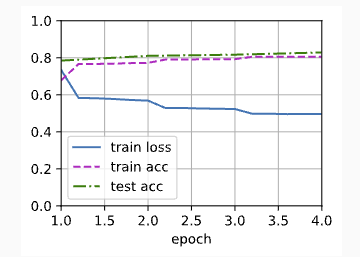
\includegraphics[height=4.1cm]{img/d2l_sentimento_rnn_treino.png}

            {\tiny Figura original do D2L, Seção 16.2.}
        \end{column}
    \end{columns}
    \begin{exampleblock}{Como ler o gráfico}
        \footnotesize
        A linha \textbf{verde} (\textit{test acc}) é a que importa: $\approx 83\%$ de acerto em críticas \textbf{nunca vistas}. Treino e teste próximos $\Rightarrow$ sem \textit{overfitting}.
    \end{exampleblock}

    \note{
        Por fim, o treino e os resultados.
        O otimizador é o Adam, com taxa de aprendizado 0,01. Ele adapta o tamanho do passo para cada parâmetro, e é muito usado em PLN por ser robusto. A perda é a entropia cruzada, que compara os dois logits com o rótulo certo, 0 ou 1. Os lotes têm 64 críticas.
        Este é o gráfico original do livro. Em azul, a perda de treino cai de cerca de 0,7 para perto de 0,49: o modelo erra cada vez menos. Em roxo tracejado, a acurácia de treino sobe até cerca de 0,80.
        E a linha verde, a acurácia no teste, é a mais importante: ela fica em torno de 0,8 e termina perto de 0,83. Isso quer dizer que o modelo acerta 83\% das críticas que nunca viu. Se a verde começasse a cair enquanto a roxa subisse, seria sinal de overfitting: o modelo teria decorado o treino. Como as duas estão próximas, o modelo está bem ajustado.
        Um detalhe curioso: o teste fica um pouco acima do treino. Isso acontece porque a acurácia de treino é a média ao longo da época, enquanto os pesos ainda estão mudando; a de teste é medida no fim da época, com o modelo já melhor.
        E, para fechar, as previsões do livro: ``this movie is so great'' sai positivo, e ``this movie is so bad'' sai negativo.
    }
\end{frame}

%========================================================================================
%  Seção 16.3 do D2L -- Sentiment Analysis: Using Convolutional Neural Networks
%  https://d2l.ai/chapter_natural-language-processing-applications/sentiment-analysis-cnn.html
%========================================================================================

%------------------------------------------------
\section{Análise de sentimento com CNN}
%------------------------------------------------

\begin{frame}{A matemática da convolução 1D}
    \begin{columns}[c]
        \begin{column}{0.44\textwidth}
            \footnotesize
            Uma \destaque{lupa de $k$ palavras} percorre a frase: em cada parada, ela multiplica o que vê pelo molde e soma.

            \vspace{0.15cm}
            \begin{itemize}\setlength{\itemsep}{3pt}
                \item \textbf{Input}: o texto já é número --- cada célula, uma palavra.
                \item \textbf{Kernel}: o \destaque{molde} de $k$ números que procura um n-grama.
                \item \textbf{Output}: um número por parada --- o encaixe daquele pedaço.
                \item Os números do kernel são \textbf{aprendidos}, não escolhidos.
            \end{itemize}
        \end{column}
        \begin{column}{0.54\textwidth}
            \centering
            \begin{tikzpicture}[font=\small,
                cel/.style={draw=dexpiBlue, fill=dexpiBlueLight, minimum width=0.85cm, minimum height=0.50cm, inner sep=0pt},
                hl/.style={draw=dexpiGreenDark, fill=dexpiGreenLight, minimum width=0.85cm, minimum height=0.50cm, inner sep=0pt, font=\small\bfseries},
                kn/.style={draw=dexpiGreenDark, fill=dexpiGreenLight, minimum width=0.85cm, minimum height=0.50cm, inner sep=0pt, font=\small\bfseries},
                lbl/.style={anchor=east, font=\scriptsize\bfseries, text=dexpiBlue}]
                \node[hl] (in0) at (0.425,0) {0};
                \node[hl] (in1) at (1.275,0) {1};
                \node[cel] (in2) at (2.125,0) {2};
                \node[cel] (in3) at (2.975,0) {3};
                \node[cel] (in4) at (3.825,0) {4};
                \node[cel] (in5) at (4.675,0) {5};
                \node[cel] (in6) at (5.525,0) {6};
                \node[lbl] at (-0.12,0) {Input};

                \node[kn] (k0) at (0.425,-1.05) {1};
                \node[kn] (k1) at (1.275,-1.05) {2};
                \node[lbl] at (-0.12,-1.05) {Kernel};
                \draw[-{Stealth}, thick, dexpiRedDark] (2.10,-1.05) -- (3.20,-1.05);
                \node[font=\scriptsize, text=dexpiRedDark, anchor=south] at (2.65,-1.05) {desliza};

                \node[hl] (out0) at (0.85,-2.10) {2};
                \node[cel] at (1.70,-2.10) {5};
                \node[cel] at (2.55,-2.10) {8};
                \node[cel] at (3.40,-2.10) {11};
                \node[cel] at (4.25,-2.10) {14};
                \node[cel] at (5.10,-2.10) {17};
                \node[lbl] at (-0.12,-2.10) {Output};

                \node[draw=dexpiBlue, fill=dexpiBlueLight, rounded corners=2pt, inner sep=4pt, font=\small] (eq) at (1.70,-3.25)
                    {${\color{dexpiBlue}0}\cdot{\color{dexpiGreenDark}1} + {\color{dexpiBlue}1}\cdot{\color{dexpiGreenDark}2} = {\color{dexpiGreenDark}\mathbf{2}}$};
                \draw[-{Stealth}, thick, dexpiGreenDark] (eq.north) -- (out0.south);
            \end{tikzpicture}

            \vspace{0.1cm}
            {\scriptsize No texto real, cada célula é um vetor de 100 números e o kernel tem 100 números por palavra; aqui usamos escalares para ver a conta.\par}
        \end{column}
    \end{columns}

    \note{
        Pensem numa lupa de duas palavras que percorre a frase. O texto já é número: 0, 1, 2, e assim por diante. Em cada parada, a lupa multiplica o que vê pelos números do molde e soma. Aqui: 0 vezes 1 mais 1 vezes 2 dá 2, o primeiro número do output. Depois ela desliza uma casa e repete. O detalhe importante: os números do molde não são escolhidos por nós --- a rede os aprende, e eles passam a disparar quando o padrão aparece.
    }
\end{frame}

\begin{frame}{A arquitetura textCNN na prática}
    \begin{columns}[c]
        \begin{column}{0.52\textwidth}
            \footnotesize
            A mesma conta, agora dentro de um modelo de verdade \cite{kim2014convolutional}.

            \vspace{0.15cm}
            \begin{itemize}\setlength{\itemsep}{3pt}
                \item A RNN lê \textbf{palavra por palavra}: o estado de hoje carrega o de ontem.
                \item A CNN olha \textbf{pedaços} de 3, 4 e 5 palavras \textbf{ao mesmo tempo}.
                \item \textbf{Fluxo}: GloVe $\to$ CNN $\to$ positivo/negativo.
                \item \textbf{Expressões locais}: ``não é bom'' é um trigrama --- a CNN o detecta como padrão.
            \end{itemize}
        \end{column}
        \begin{column}{0.44\textwidth}
            \centering
            \begin{tikzpicture}[font=\scriptsize,
                bx/.style={draw=dexpiBlue, fill=dexpiBlueLight, rounded corners=2pt, align=center, minimum width=1.85cm, minimum height=1.35cm, inner sep=2pt},
                mid/.style={draw=dexpiBlue, fill=dexpiBlue, text=white, rounded corners=2pt, align=center, minimum width=1.85cm, minimum height=1.35cm, inner sep=2pt, font=\scriptsize\bfseries}]
                \node[bx] (g) at (0,0) {Pré-treino\\{\tiny GloVe (15.5)}\\{\tiny 6 bi tokens}};
                \node[mid] (m) at (2.4,0) {Arquitetura\\{\tiny CNN (16.3)}\\{\tiny conv + max}};
                \node[bx] (a) at (4.8,0) {Aplicação\\{\tiny sentimento}\\{\tiny pos./neg.}};
                \draw[-{Stealth}, line width=1.5pt, dexpiRedDark] (g) -- (m);
                \draw[-{Stealth}, thick, dexpiBlue] (m) -- (a);
                \node[font=\tiny, text=dexpiRedDark, align=center, anchor=south] at (1.20,0.85) {aqui entra a\\convolução};
                \draw[dexpiRedDark, dashed, thick] (1.20,0.78) -- (1.20,0.06);
            \end{tikzpicture}
        \end{column}
    \end{columns}

    \vspace{0.1cm}
    \begin{exampleblock}{Por que é mais rápida}
        \footnotesize
        Todas as janelas são calculadas \textbf{em paralelo}; a RNN não pode, porque cada passo espera o anterior.
    \end{exampleblock}

    \note{
        A RNN lê palavra por palavra: o estado de hoje depende do de ontem. A CNN não: ela olha pedaços de três, quatro e cinco palavras ao mesmo tempo, e todas as janelas são calculadas em paralelo --- é por isso que ela é mais rápida. O fluxo é o desta figura: o GloVe entrega os vetores prontos, a CNN os transforma em escores, e a camada final classifica. E onde ela brilha é no local: ``não é bom'' é um trigrama, e a CNN o detecta como um padrão.
    }
\end{frame}

\begin{frame}{Max-over-time: muitos números, um resumo}
    \begin{columns}[c]
        \begin{column}{0.50\textwidth}
            \footnotesize
            Depois da convolução, cada filtro deixa uma \textbf{sequência} de escores. Como resumir a frase?

            \vspace{0.15cm}
            \begin{itemize}\setlength{\itemsep}{1pt}
                \item Para cada canal, guardamos \textbf{só o maior} escore: um número por filtro.
                \item Onde ele apareceu não importa: o filtro de ``não é bom'' dá 8 no início, no meio ou no fim.
                \item É um \destaque{filtro de importância}: o pico é a evidência de que o padrão existe.
                \item A média \textbf{diluiria} --- uma pista que aparece uma vez em 500 posições vale $1/500$; daí o \textit{global max pooling} de Collobert et al. \cite{collobert2011natural}.
            \end{itemize}
        \end{column}
        \begin{column}{0.48\textwidth}
            \centering
            \begin{tikzpicture}[font=\scriptsize]
                \foreach \v [count=\i from 0] in {1,5,2,8,3} {
                    \ifnum\i=3
                        \node[draw=dexpiGreenDark, fill=dexpiGreenLight, minimum width=0.72cm, minimum height=0.6cm, font=\scriptsize\bfseries] (v\i) at (0.95*\i,0) {\v};
                    \else
                        \node[draw=dexpiBlue, fill=dexpiBlueLight, minimum width=0.72cm, minimum height=0.6cm] (v\i) at (0.95*\i,0) {\v};
                    \fi
                }
                \node[font=\tiny, text=dexpiBlue, anchor=south] at (1.9,0.34) {escores de um filtro, um por posição};
                \draw[-{Stealth}, thick, dexpiGreenDark] (v3.south) -- (2.85,-0.62);
                \node[draw=dexpiGreenDark, fill=dexpiGreenLight, rounded corners=2pt, font=\scriptsize, anchor=north] at (2.85,-0.62) {max $=8$};
                \node[font=\tiny, text=gray, anchor=north] at (2.85,-1.18) {média $=3{,}8$};
            \end{tikzpicture}
        \end{column}
    \end{columns}

    \vspace{0.1cm}
    \begin{exampleblock}{O que o pooling compra}
        \footnotesize
        Saída de tamanho \textbf{fixo}: $C$ números, um por canal, para qualquer $T$.
    \end{exampleblock}

    \note{
        A convolução deixou uma sequência de escores por filtro: são muitos números. Para resumir, guardamos só o maior de cada canal. Reparem que a posição não importa: se o filtro procura ``não é bom'', o valor 8 diz ``achei em algum lugar'', seja no início, no meio ou no fim. É um filtro de importância. E por que não a média? Porque ela dilui: uma pista que aparece uma vez em quinhentas posições vale um quinhentos do total. O pico preserva o sinal.
    }
\end{frame}

\begin{frame}{A arquitetura completa do textCNN}
    \begin{columns}[c]
        \begin{column}{0.50\textwidth}
            \footnotesize
            O modelo de Kim (2014), de baixo para cima.

            \vspace{0.15cm}
            \begin{itemize}\setlength{\itemsep}{3pt}
                \item \textbf{Entrada}: a frase vira matriz --- 11 palavras $\times$ 6 dimensões no livro.
                \item \textbf{Filtros de larguras diferentes}: 2 e 4 no livro (3, 4 e 5 no nosso código), cada um atrás de um n-grama.
                \item \textbf{Pooling $+$ concatenação}: cada filtro vira 1 número; $4+5=9$ no exemplo.
            \end{itemize}
        \end{column}
        \begin{column}{0.48\textwidth}
            \centering
            \begin{tikzpicture}[font=\tiny]
                \fill[dexpiBlueLight] (0,0) rectangle (2.2,1.2);
                \draw[dexpiBlue!55, step=0.2] (0,0) grid (2.2,1.2);
                \node[below, font=\tiny] at (1.1,0) {11 palavras $\times$ 6};

                \fill[dexpiGreenLight] (0,1.9) rectangle (2.0,2.7);
                \draw[dexpiGreenDark!60, step=0.2] (0,1.9) grid (2.0,2.7);
                \fill[dexpiGreenLight] (2.4,1.7) rectangle (4.0,2.7);
                \draw[dexpiGreenDark!60, step=0.2] (2.4,1.7) grid (4.0,2.7);
                \node[anchor=east, font=\tiny, text=dexpiGreenDark] at (-0.05,2.3) {$k=2$};
                \node[anchor=west, font=\tiny, text=dexpiGreenDark] at (4.05,2.3) {$k=4$};

                \draw[-{Stealth}, thick, dexpiBlue] (1.0,1.2) -- (1.0,1.9);
                \draw[-{Stealth}, thick, dexpiBlue] (2.0,1.2) -- (3.0,1.7);

                \draw[-{Stealth}, dashed, thick, dexpiRedDark] (1.0,2.7) -- (1.0,3.1);
                \draw[-{Stealth}, dashed, thick, dexpiRedDark] (3.2,2.7) -- (3.2,3.1);
                \node[draw=dexpiRedDark, fill=dexpiRedLight, font=\scriptsize, minimum width=0.5cm] at (1.0,3.35) {4};
                \node[draw=dexpiRedDark, fill=dexpiRedLight, font=\scriptsize, minimum width=0.5cm] at (3.2,3.35) {5};
                \node[anchor=west, font=\tiny, text=dexpiRedDark] at (1.32,3.35) {max};
                \node[anchor=west, font=\tiny, text=dexpiRedDark] at (3.52,3.35) {max};

                \node[draw=dexpiBlue, fill=dexpiBlueLight, rounded corners=2pt, font=\tiny, inner sep=3pt] (c) at (2.1,4.0) {concat $=9$ $\rightarrow$ densa $\rightarrow$ 2};
                \draw[-{Stealth}, thick, dexpiBlue] (1.0,3.62) -- (1.55,3.82);
                \draw[-{Stealth}, thick, dexpiBlue] (3.2,3.62) -- (2.65,3.82);
            \end{tikzpicture}
        \end{column}
    \end{columns}

    \note{
        Vamos guiar o olhar de baixo para cima. Embaixo, a frase vira uma matriz: onze palavras por seis dimensões no exemplo do livro. Em cima dela, duas convoluções trabalham em paralelo: uma com filtros de duas palavras, outra com filtros de quatro. São tamanhos diferentes de propósito --- cada uma captura um n-grama diferente. As setas pontilhadas sobem para o pooling: cada canal vira um número. No fim, quatro mais cinco dão nove, que é o vetor que vai para a classificação.
    }
\end{frame}

\begin{frame}{O fluxo de dados: de $T$ palavras a 2 números}
    \begin{columns}[c]
        \begin{column}{0.48\textwidth}
            \footnotesize
            Os tamanhos, sem susto.

            \vspace{0.15cm}
            \begin{itemize}\setlength{\itemsep}{3pt}
                \item Convolução de largura $k$: a saída tem $T-k+1$ posições ($11-2+1=10$; $11-4+1=8$).
                \item O pooling reduz cada canal a \textbf{1} número; a concatenação junta todos ($4+5=9$; no nosso, $3 \times 100=300$).
                \item \textbf{Dropout} desliga neurônios ao acaso no treino; a camada densa mapeia o vetor para \textbf{2 logits}.
            \end{itemize}
        \end{column}
        \begin{column}{0.50\textwidth}
            \centering
            \begin{tikzpicture}[font=\tiny]
                \foreach \i in {0,...,8} {
                    \ifnum\i<4
                        \fill[dexpiGreenLight] ({0.30*\i},0) rectangle ++(0.27,0.27);
                        \draw[dexpiGreenDark] ({0.30*\i},0) rectangle ++(0.27,0.27);
                    \else
                        \fill[dexpiBlueLight] ({0.30*\i},0) rectangle ++(0.27,0.27);
                        \draw[dexpiBlue] ({0.30*\i},0) rectangle ++(0.27,0.27);
                    \fi
                }
                \draw[decorate, decoration={brace, amplitude=3pt, mirror}] (0,-0.05) -- (1.2,-0.05) node[midway, below=4pt] {4};
                \draw[decorate, decoration={brace, amplitude=3pt, mirror}] (1.2,-0.05) -- (2.7,-0.05) node[midway, below=4pt] {5};
                \node[anchor=south, font=\tiny, text=dexpiBlue] at (1.35,0.35) {vetor concatenado};

                \draw[-{Stealth}, thick, dexpiBlue] (2.75,0.13) -- (3.15,0.13);
                \node[draw=dexpiRedDark, dashed, fill=white, font=\tiny, minimum width=0.95cm, minimum height=0.5cm, inner sep=1pt] at (3.7,0.13) {dropout};
                \draw[-{Stealth}, thick, dexpiBlue] (4.2,0.13) -- (4.55,0.13);
                \node[draw=dexpiBlue, fill=dexpiBlueLight, font=\tiny, minimum width=0.75cm, minimum height=0.5cm, inner sep=1pt] at (4.95,0.13) {densa};
                \draw[-{Stealth}, thick, dexpiBlue] (5.35,0.13) -- (5.7,0.13);
                \node[anchor=west, font=\tiny] at (5.75,0.13) {2 logits};
            \end{tikzpicture}

            \vspace{0.15cm}
            {\scriptsize
            \begin{tabular}{@{}ll@{}}
                \toprule
                etapa & forma \\
                \midrule
                entrada & $11 \times 6$ \\
                conv $k=2$ / $k=4$ & $10 \times 4$ / $8 \times 5$ \\
                pooling & $4+5=9$ \\
                densa $+$ dropout & $2$ \\
                \bottomrule
            \end{tabular}\par}
        \end{column}
    \end{columns}

    \note{
        Agora os tamanhos, sem susto. Uma convolução de largura k sobre T palavras devolve T menos k mais um posições: onze com filtro dois dá dez; com filtro quatro, oito. O pooling reduz cada canal a um número só --- quatro mais cinco, nove. É esse vetor que entra na camada densa, passando antes pelo dropout, que desliga neurônios ao acaso no treino para o modelo não decorar. A saída são dois logits, positivo e negativo.
    }
\end{frame}

\begin{frame}[fragile]{O código do textCNN}
\begin{columns}[c]
    \begin{column}{0.62\textwidth}
\begin{lstlisting}[basicstyle=\ttfamily\fontsize{6.1}{7.1}\selectfont,aboveskip=0pt,belowskip=0pt]
class TextCNN(nn.Module):
    def __init__(self, vocab, d, ks, cs):
        super().__init__()
        self.emb = nn.Embedding(vocab, d)        # ajustavel
        self.fix = nn.Embedding(vocab, d)        # congelado
        self.convs = nn.ModuleList(
            [nn.Conv1d(2 * d, c, k) for c, k in zip(cs, ks)])
        self.pool = nn.AdaptiveMaxPool1d(1)      # max no tempo
        self.drop = nn.Dropout(0.5)
        self.out = nn.Linear(sum(cs), 2)

    def forward(self, inputs):                   # (B, T)
        E = torch.cat((self.emb(inputs), self.fix(inputs)), dim=2)
        E = E.permute(0, 2, 1)                   # (B, 200, T)
        H = [self.pool(torch.relu(c(E))).squeeze(-1)
             for c in self.convs]                # 3 x (B, 100)
        return self.out(self.drop(torch.cat(H, dim=1)))  # (B, 2)

d, ks, cs = 100, [3, 4, 5], [100, 100, 100]
\end{lstlisting}
    \end{column}
    \begin{column}{0.34\textwidth}
        \footnotesize
        \textbf{Onde está cada ideia}
        \begin{enumerate}\setlength{\itemsep}{2pt}
            \item \texttt{emb} $+$ \texttt{fix}: os 200 canais.
            \item \texttt{Conv1d}: um detector por canal e por largura.
            \item \texttt{pool}: o máximo no tempo, um número por canal.
            \item \texttt{cat} $+$ \texttt{out}: 300 números $\to$ 2 logits.
        \end{enumerate}
        \vspace{0.15cm}
        {\scriptsize\color{dexpiRedDark} GloVe: \texttt{copy\_} nas duas tabelas e \texttt{requires\_grad = False} em \texttt{fix}.}
    \end{column}
\end{columns}

\note{
    Este é o código, com os nomes encurtados. No construtor, as duas tabelas, a lista de convoluções, o pooling, o dropout e a camada de saída. No forward: concatenamos as duas tabelas, transpomos, aplicamos cada convolução com ReLU e pooling, e concatenamos os resultados.
    Uma observação para quem for comparar com o livro: o texto chama o pooling de max-over-time, mas o listing em PyTorch do D2L traz AdaptiveAvgPool1d, que faz média. Aqui usamos o máximo, que é o que o texto descreve; se você reproduzir o código do livro como está, vai treinar com média.
    Os hiperparâmetros são os do livro: embedding de 100, larguras 3, 4 e 5, 100 canais, dropout 0,5, Adam com taxa 10 menos 3, 5 épocas.
}
\end{frame}

\begin{frame}{Resultados: CNN $\times$ BiRNN, e os limites}
    \begin{columns}[c]
        \begin{column}{0.46\textwidth}
            \centering
            \footnotesize
            \begin{tabular}{lcc}
                \toprule
                 & BiRNN & textCNN \\
                \midrule
                perda de treino & $\approx 0{,}49$ & $0{,}066$ \\
                acurácia treino & $\approx 0{,}80$ & $0{,}979$ \\
                acurácia teste & $\approx 0{,}83$ & $\mathbf{0{,}868}$ \\
                \bottomrule
            \end{tabular}
            \vspace{0.15cm}
            {\scriptsize IMDb; GloVe, $d = 100$; CNN: Adam, $\text{lr}=10^{-3}$, 5 épocas.}
        \end{column}
        \begin{column}{0.50\textwidth}
            \footnotesize
            \begin{itemize}\setlength{\itemsep}{2pt}
                \item O teste sobe de $\approx 0{,}83$ para $\mathbf{0{,}868}$, com os mesmos dados e o mesmo GloVe; mudam a arquitetura e a taxa ($10^{-3}$ contra $10^{-2}$).
                \item \textbf{O alarme}: treino $0{,}98$ contra teste $0{,}87$. A CNN decora mais --- \texttt{dropout} $0{,}5$ e metade dos embeddings congelada são as defesas.
                \item \textbf{Por que funciona}: o \textit{max} ignora \textbf{onde} a pista está; ``is so great'' vale no começo ou no fim.
            \end{itemize}
        \end{column}
    \end{columns}

    \vspace{0.1cm}
    \begin{alertblock}{O limite da janela}
        \footnotesize
        Um filtro de 3 palavras não liga ``apesar do começo lento'' a ``é ótimo'' no fim de uma crítica longa. Por isso Kim usa 3, 4 e 5; a evolução natural é a \textbf{atenção} (BERT, Seção 15.8), que liga qualquer posição a qualquer outra.
    \end{alertblock}

    \note{
        Agora a comparação, com os números do livro. A BiRNN chega a cerca de 83 por cento de acurácia no teste, com perda de treino de 0,49. O textCNN chega a 86,8, com perda de 0,066. Os mesmos dados e os mesmos embeddings; mudam a arquitetura e a taxa de aprendizado, 10 menos 3 no lugar de 10 menos 2.
        Mas olhem a distância entre treino e teste: 0,98 contra 0,87. A CNN decora boa parte do treino. As duas defesas estão no modelo: o dropout de 0,5 e a metade congelada dos embeddings. E vale lembrar que a acurácia de treino da RNN era medida ao longo da época, então a comparação de gap não é perfeitamente limpa; o que importa é o teste.
        O limite é estrutural: um filtro de 3 palavras só vê 3 palavras. Ele não liga "apesar do começo lento" a "é ótimo" no fim de uma crítica longa. A solução de Kim é ter filtros de 3, 4 e 5; a solução seguinte, e a que domina hoje, é a atenção: cada posição olha todas as outras, que é exatamente o BERT que vimos na seção 15.8.
    }
\end{frame}


%------------------------------------------------

\begin{frame}[allowframebreaks]
\frametitle{Referências}
    \footnotesize
    \nocite{*}
    \bibliographystyle{ieeetr}
    \bibliography{reference.bib}
\end{frame}

%------------------------------------------------

\begin{frame}
    \Huge{\centerline{\textbf{Chegamos ao Fim}}}
    \Huge{\centerline{\textbf{Obrigado pela sua Atenção}}}
\end{frame}

%------------------------------------------------
%  Backup: slides de detalhe, para usar só se perguntarem
%------------------------------------------------

%========================================================================================
%  Backup -- slides que saíram do fluxo principal (detalhe de implementação)
%  Ficam depois do "obrigado", para usar só se perguntarem ou se sobrar tempo.
%========================================================================================

% Células coloridas da tabela do minibatch (contexto em verde, ruído em vermelho)
\newcommand{\ctxcell}[1]{\colorbox{dexpiGreenLight}{\color{dexpiGreenDark}\textbf{#1}}}
\newcommand{\ruidocell}[1]{\colorbox{dexpiRedLight}{\color{dexpiRedDark}\textbf{#1}}}

\section{Backup}

\begin{frame}{O minibatch: quatro tensores}
    \small
    \begin{itemize}
        \item Cada exemplo tem um número diferente de contextos e ruídos. Para formar um tensor, completamos com \textbf{zeros} (\textit{padding}).
        \item Exemplo do livro: centro 1, contextos {\color{dexpiGreenDark}\textbf{2}}, ruídos {\color{dexpiRedDark}\textbf{3}}.
    \end{itemize}
    \vspace{0.1cm}
    \centering
    \begin{tabular}{l|cccccc|l}
        \toprule
        \texttt{centers} & \multicolumn{6}{c|}{\texttt{contexts\_negatives}} & \\
        \midrule
        1 & \ctxcell{2} & \ctxcell{2} & \ruidocell{3} & \ruidocell{3} & \ruidocell{3} & \ruidocell{3} & exemplo 1 \\
        1 & \ctxcell{2} & \ctxcell{2} & \ctxcell{2} & \ruidocell{3} & \ruidocell{3} & 0 & exemplo 2 \\
        \midrule
        \texttt{labels} & 1 & 1 & 0 & 0 & 0 & 0 & \\
                        & 1 & 1 & 1 & 0 & 0 & 0 & \\
        \midrule
        \texttt{masks}  & 1 & 1 & 1 & 1 & 1 & 1 & \\
                        & 1 & 1 & 1 & 1 & 1 & {\color{dexpiRedDark}\textbf{0}} & $\leftarrow$ padding \\
        \bottomrule
    \end{tabular}

    \vspace{0.2cm}
    \raggedright
    \begin{columns}[t]
        \begin{column}{0.48\textwidth}
            \footnotesize
            \begin{itemize}
                \item \texttt{labels}: \textbf{1} = contexto (positivo), \textbf{0} = ruído ou padding.
                \item \texttt{masks}: \textbf{0} marca o padding, que a perda deve ignorar.
            \end{itemize}
        \end{column}
        \begin{column}{0.48\textwidth}
            \footnotesize
            \textbf{Formatos no PTB} (lote de 512):\\
            \texttt{centers}: $512 \times 1$\\
            os outros três: $512 \times 60$
        \end{column}
    \end{columns}

    \note{
        Como os exemplos entram no modelo? Em minibatches de quatro tensores. O problema é que cada centro tem um número diferente de palavras de contexto, porque a janela é sorteada, e portanto um número diferente de ruídos. Para empilhar os exemplos num tensor retangular, completamos as linhas mais curtas com zeros: é o padding.
        Este é o exemplo do próprio livro. Os dois exemplos têm centro 1. O primeiro tem 2 contextos e 4 ruídos; o segundo tem 3 contextos e 2 ruídos, então ganha um zero no final.
        \texttt{contexts\_negatives} junta, na mesma linha, os contextos, em verde, e depois os ruídos, em vermelho. \texttt{labels} diz qual é qual: 1 para contexto, 0 para ruído. \texttt{masks} diz o que é real e o que é padding: o zero no final do exemplo 2 é padding e não pode entrar na perda.
        No PTB, com lotes de 512 exemplos, \texttt{centers} tem formato 512 por 1, e os outros três têm 512 por 60: 60 é o comprimento da linha mais longa do lote.
    }
\end{frame}

\begin{frame}[fragile]{O laço de treino}
\vspace{-0.2cm}
\begin{lstlisting}[basicstyle=\ttfamily\fontsize{6.2}{7.0}\selectfont]
embed_size = 100
net = nn.Sequential(nn.Embedding(len(vocab), embed_size),   # net[0]: vetores de centro v
                    nn.Embedding(len(vocab), embed_size))   # net[1]: vetores de contexto u

def train(net, data_iter, lr, num_epochs, device):
    net.apply(init_weights)                                 # inicializacao Xavier
    optimizer = torch.optim.Adam(net.parameters(), lr=lr)
    for epoch in range(num_epochs):
        for center, context_negative, mask, label in data_iter:
            pred = skip_gram(center, context_negative, net[0], net[1])   # (B, 1, 60)
            l = (loss(pred.reshape(label.shape).float(), label.float(), mask)
                 / mask.sum(axis=1) * mask.shape[1])                     # ignora o padding
            optimizer.zero_grad()
            l.sum().backward()
            optimizer.step()

lr, num_epochs = 0.002, 5
train(net, data_iter, lr, num_epochs)
\end{lstlisting}
\vspace{-0.2cm}
\footnotesize
\textbf{Hiperparâmetros}: lote 512, janela máx. 5, $K = 5$, $d = 100$, Adam com $\text{lr} = 0{,}002$, 5 épocas.\\
\textbf{Saída do livro}: {\color{dexpiGreenDark}\texttt{loss 0.410}}, cerca de 223 mil \textit{tokens}/s numa GPU.

\note{
    Este é o laço de treino, com o código do livro levemente resumido.
    O modelo são as duas tabelas de embeddings de dimensão 100. Antes de treinar, os pesos são inicializados com Xavier, e o otimizador é o Adam.
    Para cada minibatch: calculamos os escores com o skip-gram, que dá o formato B por 1 por 60. Achatamos para o formato dos rótulos e calculamos a perda binária com a máscara. A divisão por \texttt{mask.sum} e a multiplicação por \texttt{mask.shape[1]} fazem a média só sobre as entradas reais, ignorando o padding. Depois vem o passo de sempre: zerar os gradientes, retropropagar e atualizar os pesos.
    Com taxa de aprendizado 0,002 e 5 épocas, a perda final no livro é 0,410, processando cerca de 223 mil tokens por segundo numa GPU. Para comparação, um classificador que chuta 50\% em cada par teria perda $\log 2 \approx 0{,}69$.
}
\end{frame}


\end{document}
